% -*- root: ../GeometriaDiferencial.tex -*-

\section{Formas diferenciales}

La teoría de este tema se encuentra en el \fref{chap:FormasDiferenciales}. Ejercicios recomendados correspondientes a \cite[Capítulo 1]{doCarmo94}.

\begin{problem}[4] Sea ω una $k$-forma en $\real^n$, donde $k$ es impar. Demuestra que $ω \y ω = 0$.
\label{ej:T1_E4}
\solution

\doneby{Pedro}

\approvedby{Dejuan}

Puesto que ω es una k-forma tenemos que

\[ω = \sum a_i \dif x_{i_1}...\dif x_{i_k} \text{ con k impar}\]

Al calcular el producto exterior de esta forma consigo misma vamos a obtener una suma donde cada sumando aparece dos veces si reordenamos los diferenciables.

\paragraph{Si $2k > n$:\\}
Para empezar, es posible que estos sumandos sean 0 directamente, cosa que ocurre si estamos en un espacio de dimensión menor que 2k y en este caso no habría nada más que hacer. Esto ocurre si multiplicamos dos 2-formas en $\real^3$ puesto que cada sumando del resultado tendrá un producto de 4 diferenciales escogidos de un conjunto de 3 posibles. Por el principio del palomar es claro que habremos tomado al menos uno repetido, por lo que obtendremos un 0 directamente ($dx ∧ dx = 0$).

\paragraph{Si $2k≤n$:\\}
Por tanto sólo nos queda ver el caso en que estos sumanos no se hagan 0. Entonces nos quedaría, en alguna parte del resultado final, la suma:
\[a_i \dif x_{i_1}...\dif x_{i_k} \cdot a_j \dif x_{j_1}...\dif x_{j_k} + a_j \dif x_{j_1}...\dif x_{j_k} \cdot a_i \dif x_{i_1}...\dif x_{i_k}\]

Para poder sumar correctamente debemos escribir en ambos sumandos los diferenciales en el mismo orden. Para ello tomamos el segundo sumando y desplazamos el primer diferencial hasta el final. Esto nos supone un número par de intercambios para llevarlo al final de los $\dif x_j$ más un número impar de intercambios para llevarlo hasta el final de los $\dif x_i$.\footnote{Poneos un ejemplo de 3 diferenciales o de 4 (para el primer caos y el segundo respectivamente) y veis que tengo razón}.

Con esto podemos ver que mover la primera diferencial del segundo sumando hasta el final implica cambiar de signo este sumando, pues hacemos un número impar de intercambios. Puesto que esta operación la tenemos que hacer $k$ veces siendo $k$ un número impar, es claro que nos quedará el segundo sumando de signo negativo.

Por tanto la suma escrita anteriormente será 0 y al multiplicar una forma por sí misma no habrá ningún termino libre (que no esté emparejado con otro formando una suma con la indicada) por lo que es claro que queda 0.

Si queremos escribirlo más formalmente:

\begin{align*}
φ ∧ φ &= \sum_{I,J} a_I · a_J \; \dif x_I ∧ \dif x_J = \\
& \sum_{i_1,...,i_k} \sum_{j_i,...,j_k} a_{i_1,...,i_k} · a_{j_1,...,j_k} \; \dif x_{i_1} ∧ ... ∧ \dif x_{i_k} ∧ \dif x_{j_1} ∧ ... ∧ \dif x_{j_k} \overset{*}{=} \\
\sum_{i_1,...,i_k}& \sum_{j_i<i_1,...,j_k<i_k} (a_{i_1,...,i_k}a_{j_1,...,j_k} + (-1)^k a_{j_1,...,j_k}a_{i_1,...,i_k}) \dif x_{i_1} ∧ ... ∧ \dif x_{i_k} ∧ \dif x_{j_1} ∧ ... ∧ \dif x_{j_k} =\\
& \sum_{I,J<I} (a_Ia_J + (-1)^ka_Ja_I) \dif x_I∧\dif x_J  \overset{k \text{ impar}}{=}0
 \end{align*}

\textbf{*}: Por la explicación de Pedro.

\end{problem}

\begin{problem}[5] Sean $φ,ψ,θ$ las siguientes formas diferenciales en $ℝ^3$:
\begin{align*}
φ &= x \dif x - y \dif y \\
ψ &= z \dif x \y \dif y + x \dif y \y \dif z \\
θ &= z \dif y
\end{align*}

Calcula:
\ppart $φ\y ψ$.
\ppart $θ\y φ \y ψ$.
\ppart $\dif φ$.
\ppart $\dif ψ$.
\ppart $\dif θ$.

\solution

\doneby{Pedro}

\approvedby{Dejuan}

\spart
\[φ\y ψ = xz \ \dif x \y \dif x \y \dif y \ + \ x^2 \dif x \y \dif x \y \dif z \ - yz \ \dif y \y \dif x \y \dif y \ - yx \ \dif y \y \dif y \y \dif z = x^2 \ \dif x \y \dif y \y \dif z\]

\spart
\[θ\y φ \y ψ= 0\]

Es fácil de ver apoyándonos en el apartado a) y en la propiedad asociativa del producto exterior. La otra forma de verlo es pensando que el resultado será una $1+2+1 = 4$-forma en $\real^3$ que tiene que tener algún $\dif (algo)$ repetido.

\spart
\[\dif φ=\dif x \y \dif x + 0\cdot \dif y \y \dif x+0\cdot \dif z \y \dif x = 0\]

\spart
\[\dif ψ=\dif z \y \dif x \y \dif y + \dif x \y \dif y \y \dif z = 2 \cdot \dif x \y \dif y \y \dif z \]

\spart
\[\dif θ= \dif z \y \dif y = - \dif y ∧ \dif z\]

\end{problem}

\begin{problem}[6] Sea $\appl{f}{U⊂ℝ^m}{ℝ^n}$ una aplicación diferenciable. Supongamos que $m < n$ y sea ω una $k$-forma en $ℝ^n$, con $k > m$. Demuestra que $f^*ω = 0$.
\solution

\doneby{Pedro}

Primero vamos a pensar en qué es lo que tendríamos que hacer para calcular este pull back.

Dada la función $f$ podemos escribir cada coordenada de $\real^n$ como combinación de funciones de las variables de $\real^m$.

Podemos escribir
\[ω = \sum a_i(x_1,...x_n) \dif x_{i_1}.... \dif x_{i_k}\]

Al aplicar el pull back sustituimos cada $a_i(x_1,...x_n)$ por $a_i(Im (f)_1,...Im(f)_n)$, con lo que obtendremos otros coeficientes, cosa que nos da igual para este ejercicio.

El detalle importante es lo que vamos a hacer con los diferenciales. Vamos a sustituir cada uno de ellos por $\dif Im(f)_i$ considerando esta imagen como una 0-forma a la hora de derivar.

Finalmente, cuando escribamos el producto de todos los $\dif x_i$ posiblemente nos quedará un producto de formas que dará lugar a un sumatorio. El detalle a recalcar es que cada producto implicará multiplicar $k$ diferenciales escogidas entre un conjunto de $m<k$ posibles diferenciales.

De nuevo aplicamos el principio del palomar y vemos que en todos estos productos estaremos cogiendo alguna diferencial varias veces con lo que nos quedará una suma de 0.

Finalmente $a_i \cdot 0 = 0$.

\doneby{Dejuan}

El pull back (por definición) nos lleva $k$-formas de un sitio a $k$-formas en otro. En este caso nos llevará una $k$-forma a $\real^m$ con $k>m$. Entonces, por el principio del Palomar tiene que haber algún $\dif (algo)$ repetido

\end{problem}

\begin{problem}[7] Sea $ω$ la 2-forma en $ℝ^{2n}$ dada por \[ ω = \dif x_1 \y \dif x_2 + \dif x_3 \y \dif x_4 + \dotsb + \dif x_{2n-1} \y \dif x_{2n} \]

Calcula el producto exterior de $n$ copias de ω (esto es, $ω \underbracket{\y \dotsb \y}_{n} ω$).
\solution

\doneby{Dejuan}

\approvedby{Pedro}

Antes de nada podemos ver que ese producto nos dará una suma de 2n-formas que tendremos que calcular.

Todas las 2n-formas que se obtengan al multiplicar uno de los sumandos de ω por sí mismo será 0. Por tanto sólo sobrevivirán aquellos sumanos que combinen todos los posibles alores de $\dif x_i$.\footnote{Si no combina todos los valores posibles pero tiene 2n elementos, por necesidad está repitiendo algún elemento, por lo que quedará 0}.

Nos quedarán $n!$ factores, cada uno con una ordenación diferente de los pares $\dif x_i \y \dif x_{i+1}$ de ω. Como cualquier reordenación que tengamos que hacer implicará mover directamente dos diferenciales, implicará un número par de cambios $2\cdot k$ por lo que se mantendrá el signo.


Vamos a estudiar el caso $n=2$ para verlo más claro.

Tenemos \[ω=\dif x_1 ∧ \dif x_2 + \dif x_3 ∧ \dif x_4 \]

y al multiplicar esta forma consigo misma obtenemos:
\[ ω∧ω = \dif x_1 ∧ \dif x_2 ∧ \dif x_3 ∧ \dif x_4 + \dif x_3 ∧ \dif x_4 \y \dif x_1 ∧ \dif x_2 = 2 \dif x_1 ∧ \dif x_2 ∧ \dif x_3 ∧ \dif x_4\]

El resultado final será:

\[
ω \underbracket{\y \dotsb \y}_{n} ω = n! \dif x_1 ∧ ... ∧ \dif x_{2n}
\]


\end{problem}

\begin{problem}[8] Sea $\appl{f}{ℝ^n}{ℝ^n}$ la aplicación diferenciable dada por $f(x_1, \dotsc, x_n) = (y_1, \dotsc, y_n)$, y sea $ω = \dif y_1 \y \dotsb \y \dif y_n$. Demuestra que \[ f^* ω = \det (\dif f) · \dif x_1 \y \dotsb \y \dif x_n \]
\solution

\doneby{Dejuan}

Recordamos\footnote{consultando los magníficos apuntes de Análisis Matemático en donde viene muy bien el pull-back con ejemplos} que $f^* (ω∧φ) = f^*(ω) ∧ f^*(φ)$.

Sabemos además\footnote{Reconsultando Análisis Matemático o el doCarmo} que $f^*(\dif y_1) = \dif x_1 (y_1,...,y_n) = \displaystyle\sum \dpa{}{x_i}f_1 \dif x_i$.

Juntando estos 2 conocimientos, escribimos:

\[
f^*(ω) = f^*(\dif y_1) ∧ ... ∧ f^*(\dif y_n) = \left(\sum_i \dpa{f_1}{x_i}\dif x_i\right) ∧ ... ∧ \left( \sum_i \dpa{f_n}{x_i} dx_i\right)
\]

Ahora sólo es cuestión de reorganizar los términos para intentar escribirlo como determinante.


Vamos a demostrarlo por inducción.

El caso base es $n=2$:
\begin{align*}
f^*(y_1 ∧ y_2) &= f^*(y_1) ∧ f^*(y_2) = \left(\dpa{f_1}{x_1}\dif x_1 + \dpa{f_1}{x_2} \dif x_2 \right)∧  \left(\dpa{f_2}{x_1}\dif x_1 + \dpa{f_2}{x_2} \dif x_2 \right) = \\
&= \left(\dpa{f_1}{x_2} · \dpa{f_1}{x_1} \dif x_1 ∧ \dif x_2\right) + \left(\dpa{f_1}{x_2} · \dpa{f_2}{x_1} \dif x_2 ∧ \dif x_1\right) = \\
&= \left(\dpa{f_2}{x_2} · \dpa{f_1}{x_1} - \dpa{f_1}{x_2} · \dpa{f_2}{x_1}\right) \dif x_1 ∧ \dif x_2 = \\
&=\det(\dif f_n) \dif x_1 ∧ \dif x_2
\end{align*}

Ahora, suponiendo cierto que
\[
\left(\sum_i^n \dpa{f_1}{x_i}\dif x_i\right) ∧ ... ∧ \left( \sum_i^n \dpa{f_n}{x_i} dx_i\right) = \det(df_n) \dif x_1 ∧ ... ∧ \dif x_n
\]
vamos a ver que

\[
\left(\sum_i^{n+1} \dpa{f_1}{x_i}\dif x_i\right) ∧ ... ∧ \left( \sum_i^{n+1} \dpa{f_{n+1}}{x_i} dx_i\right) = \det(df_n) \dif x_1 ∧ ... ∧ \dif x_n
\]

Para ello, el primer sumando lo extendemos y aplicamos la propiedad distributiva y utilizando que $\dif x∧\dif x = 0$\footnote{es por esto por lo que los sumatorios comienzan en 2}, es decir:

\begin{align*}
&\dpa{f_1}{x_1} \dif x_1 ∧ \underbrace{\left [ \left( \sum_{i=2}^{n+1} \dpa{f_2}{x_i} \dif x_i \right) ∧ ... ∧ \left( \sum_{i=2}^{n+1} \dpa{f_{n+1}}{x_i} \dif x_i \right)\right]}_{\det (d(f_2,..,f_{n+1}))}  + \dpa{f_2}{x_2}\dif x_2 ∧ (...) + ... =\\
&\sum_{i=1}^{n+1} \dpa{f_1}{x_i} \dif x_i · \left[\det\left(d(f_1,...,f_{i-1},f_{i+1},...,f_n)\right) \dif x_1 ∧ ... ∧ \dif x_{i-1} ∧ \dif x_{i+1} ∧ ... ∧ \dif x_n\right] \overset{*}{=}\\
&\det(\dif (f_{n+1})) \dif x_1 ∧ \dif x_{n+1}
\end{align*}

\textbf{*:} Por cómo se calculan los determinantes utilizando menores, es decir:

\begin{align*}
\begin{vmatrix} a & b & c & d\\e & f & g & h\\i & j & k & l\\m & n & o & p \end{vmatrix} = a\begin{vmatrix} f & g & h\\j & k & l\\n & o & p \end{vmatrix} -b\begin{vmatrix} e & g & h\\i & k & l\\m & o & p \end{vmatrix}+c\begin{vmatrix} e & f & h\\i & j & l\\m & n & p \end{vmatrix}-d\begin{vmatrix} e & f & g\\i & j & k\\m & n & o \end{vmatrix}
\end{align*}

Y los signos negativos aparecen al desplazar el $\dif x_i$ a su posición correspondiente, teniendo que realizar $i$ cambios.

% % % Sólo tenemos que ver que ese algo largo sea el determinante. Para ello, nos ayudamos de escribir la cuenta que tenemos sin sumatorios, donde $a_{ij} =\displaystyle \dpa{f_i}{x_j}$
% % %
% % % \begin{align*}
% % % &(a_{11}\dif x_1 + a_{12} \dif x_2 +  \cdots + a_{1n}\dif x_n) \;∧ \\
% % % &(a_{21}\dif x_1 + a_{22} \dif x_2 +  \cdots + a_{2n}\dif x_n) \;∧ \\
% % % & \quad \vdots\\
% % % &(a_{n1}\dif x_1 + a_{22} \dif x_2 +  \cdots + a_{nn}\dif x_n)\\
% % % \end{align*}
% % %
% % % Por otro lado, en \href{http://en.wikipedia.org/wiki/Determinant}{Wikipedia} encontramos una fórmula de desarrollo de determinantes de matrices $n$-dimensionales (la fórmula de Leibniz)
% % %
% % % \[
% % % \det(A) = \sum_{\sigma \in S_n} \text{sgn}(\sigma) \prod_{i=1}^n a_{i,\sigma_i}
% % % \]
% % % donde $S_n$ es nuestro queridísimo grupo simétrico\footnote{el conjunto de todas las permutaciones de listas de n elementos} que veíamos en Galois. Esta fórmula sale de la generalización de lo que ya conocemos:
% % % \begin{equation*}
% % % \begin{vmatrix} a & b & c & d\\e & f & g & h\\i & j & k & l\\m & n & o & p \end{vmatrix} = a\begin{vmatrix} f & g & h\\j & k & l\\n & o & p \end{vmatrix} -b\begin{vmatrix} e & g & h\\i & k & l\\m & o & p \end{vmatrix}+c\begin{vmatrix} e & f & h\\i & j & l\\m & n & p \end{vmatrix}-d\begin{vmatrix} e & f & g\\i & j & k\\m & n & o \end{vmatrix}
% % % \end{equation*}
% % %
% % %
% % % El siguiente paso que se me ocurre dar es demostrarlo por inducción.


\end{problem}

\begin{problem}[18] Una función $\appl{g}{ℝ^3}{ℝ}$ es homogénea de grado $k$ si \[ g(tx,ty,tz) = t^k g(x,y,z)\] para $t > 0$ y $(x,y,z) ∈ ℝ^3$. Demuestra que

\ppart Si $g$ es diferenciable y homogénea de grado $k$, entonces \[ x \dpa{g}{x} + y \dpa{g}{y} + z \dpa{g}{z} = k g\]

Esta es la relación de Euler.

\textit{Sugerencia}: deriva $g(tx,ty,tz) = t^k g(x,y,z)$ con respecto a $t$ y supón $t = 1$.

\ppart Si la forma diferencial \[ ω = a \dif x + b \dif y + c \dif z \] es tal que $a,b,c$ son funciones homogéneas de grado $k$ y se tiene que $\dif ω = 0$, entonces $ω = \dif f$ con \[ f = \frac{xa + yb + zc}{k+1}\]

\textit{Sugerencia}: $\dif ω = 0$ implica que \[ \dpa{b}{x} = \dpa{a}{y},\quad \dpa{c}{x} = \dpa{a}{z},\quad \dpa{b}{z} = \dpa{c}{y} \] y aplica la relación de Euler del anterior apartado.

\ppart Si la forma diferencial \[ σ = a \dif y \y \dif z + b \dif z \y \dif x + c \dif x \y \dif y \] es tal que $a,b,c$ son homogéneas de grado $k$ y $\dif σ = 0$, entonces $σ = \dif γ$ donde \[ γ = \frac{(zb-yc) \dif x + (xc-za) \dif y + (ya-xb) \dif z}{k+2} \]
\solution

\doneby{Pedro}

\spart

Atendiendo a la sugerencia proporcionada derivamos $g(tx,ty,tz)=t^k g(x,y,z)$ respecto de $t$ a ambos lados de la igualdad obteniendo:
\[x\frac{\partial g}{\partial x}+y\frac{\partial g}{\partial y}+z\frac{\partial g}{\partial z} = k t^{k-1}g(x,y,z)\]

Si tomamos $t=1$ ya tenemos el resultado buscado.

\spart

Vamos a calcular la diferencia de la función $f$ dada y a ver si coincide cono ω bajo la suposición $\dif w = 0$.

\[\dif f = \dif \frac{xa(x,y,z)+yb(x,y,z)+zc(x,y,z)}{k+1}=\]
\[=\frac{(a(x,y,z)+xa_x(x,y,z)+yb_x(x,y,z)+zc_x(x,y,z))\dif x}{k+1}+\]
\[+\frac{(b(x,y,z)+yb_y(x,y,z)+xa_y(x,y,z)+zc_y(x,y,z)) \dif y}{k+1}+\]
\[+\frac{(c(x,y,z)+zc_z(x,y,z)+yb_z(x,y,z)+xa_z(x,y,z)) \dif z}{k+1}\]

Hasta aquí simplemente hemos derivado. Basándonos en la información que nos da la sugerencia sobre lo que se puede deducir de que $\dif ω = 0$, las relaciones entre las derivadas parciales, podemos escribir:

\[\dif f = \dif \frac{xa(x,y,z)+yb(x,y,z)+zc(x,y,z)}{k+1}=\]
\[=\frac{(a(x,y,z)+xa_x(x,y,z)+ya_y(x,y,z)+za_z(x,y,z))\dif x}{k+1}+\]
\[+\frac{(b(x,y,z)+yb_y(x,y,z)+xb_x(x,y,z)+zb_z(x,y,z)) \dif y}{k+1}+\]
\[+\frac{(c(x,y,z)+zc_z(x,y,z)+yc_y(x,y,z)+xc_x(x,y,z)) \dif z}{k+1}\]

Basándonos ahora en la propiedad que hemos probado en el apartado anterior, tenemos:

\[\dif f = \dif \frac{xa(x,y,z)+yb(x,y,z)+zc(x,y,z)}{k+1}=\]
\[=\frac{(a(x,y,z)+ka(x,y,z))\dif x}{k+1}+\frac{(b(x,y,z)+kb(x,y,z)) \dif y}{k+1}+\frac{(c(x,y,z)+kc(x,y,z)) \dif z}{k+1}=\]
\[= a(x,y,z)\dif x + b(x,y,z) \dif y + c(x,y,z) \dif z = ω\]

\spart

Puesto que $\dif σ=0$ tenemos:
\[a_x(x,y,z)+b_y(x,y,z)+c_z(x,y,z) = 0\]

De forma similar a lo que hicimos en el apartado anterior vamos a derivar γ, aunque esta vez no vamos a escribir todos los pasos de forma tan exhaustiva.

\[\dif γ = \frac{(zb_y-c-yc_y-c-xc_x+za_x)\dif y \y \dif x + (b+zb_z-yc_z-ya_x+b+xb_x) \dif z \y \dif x}{k+2}+\]
\[+\frac{(a+ya_y-xb_y-xc_z+a+za_z)\dif y \y \dif z}{k+2}=\]
utilizando $a_x+b_y+c_z=0$:
\[\dif γ = \frac{(-c-yc_y-c-xc_x-zc_z)\dif y \y \dif x + (b+zb_z-yb_y+b+xb_x) \dif z \y \dif x}{k+2}+\]
\[+\frac{(a+ya_y+xa_y+a+za_z)\dif y \y \dif z}{k+2}=\]
y basándonos ahora otra vez más en el primer apartado tenemos:
\[\dif γ = c \dif x \y \dif y + b \dif z \y \dif x + a \dif y \y \dif z = σ\]


\end{problem}




%%%%%%%%%%%%%%%%%%%%%%%%%%%%%%%%%%%%%%%%%%%%%%%%%%%%%%%%%%%%%%%%%%%%%%%%%%%%%%%%%%%%%%%%%%%%%%%%%%%%
%%%%%%%%%%%%%%%%%%%%%%%%%%%%%%%%%%%%%%%%%%%%%%%%%%%%%%%%%%%%%%%%%%%%%%%%%%%%%%%%%%%%%%%%%%%%%%%%%%%%
%%%%%%%%%%%%%%%%%%%%%%%%%%%%%%%%%%%%%%%%%%%%%%%%%%%%%%%%%%%%%%%%%%%%%%%%%%%%%%%%%%%%%%%%%%%%%%%%%%%%
%%%%%%%%%%%%%%%%%%%%%%%%%%%%%%%%%%%%%%%%%%%%%%%%%%%%%%%%%%%%%%%%%%%%%%%%%%%%%%%%%%%%%%%%%%%%%%%%%%%%
%%%%%%%%%%%%%%%%%%%%%%%%%%%%%%%%%%%%%%%%%%%%%%%%%%%%%%%%%%%%%%%%%%%%%%%%%%%%%%%%%%%%%%%%%%%%%%%%%%%%


\section{Integrales de línea}

La teoría correspondiente a estos ejercicios se encuentra en la \fref{sec:IntegralesLinea}. Ejercicios de \cite[Capítulo 2]{doCarmo94}.

\begin{problem}[1] Demuestra que la forma $ω =  2xy^3\dif x + 3 x^2 y^2 \dif y$ es cerrada y calcula $\int_c ω$, donde $c$ es el arco de la parábola $y = x^2$ desde $(0,0)$ hasta $(x,y)$.
\solution

\doneby{Pedro}

Una forma diferencial será cerrada si su derivada es 0. Por tanto para demostrar que ω es cerrada basta con ver que $\dif ω = 0$.

\[\dif ω = 2x3y^2 \dif y \y \dif x +6x y^2 \dif x \y \dif y = 0\]

Podemos ver que ω es una forma exacta, pues $f=x^2y^3$ es una 0-forma tal que $\dif f = ω$.

El arco de parábola dado podemos verlo como una función $\appl{c}{\real}{\real^2}$ tal que $c(t)=(t,t^2)$.

Por tanto podemos calcular la integral como:
\[\int_c ω = \int_c \dif f = \int_0^{x} c^*(\dif f) = f(c(x))-f(c(0))=x^8-0 = x^8 \]

\end{problem}

\begin{problem}[2]\label{ej:IntegralesLinea2}
\ppart Demuestra que si $ω$ es una $1$-forma diferenciable definida en $U ⊂ ℝ^n$, $\appl{c}{[a,b]}{U}$ es una curva diferenciable y $\abs{ω(c(t))} ≤ M$ para todo $t ∈ [a,b]$, entonces \[ \abs{\int_c ω} ≤ ML \] donde $L$ es la longitud de $c$.

\ppart Sea $ω$ una 1-forma cerrada en $ℝ^2 \setminus \set{0}$. Suponemos que $ω$ está acotada (esto es, sus coeficientes están acotados) en un disco de centro el origen. Demuestra que $ω$ es exacta en $ℝ^2 \setminus \set{0}$.

\ppart Demuestra que el resultado del apartado anterior es cierto si sólo suponemos que $\dif  ω = 0$ y que \[ \lim_{x^2+y^2  \to 0} ω\sqrt{x^2+y^2} = 0 \]
\solution

\doneby{Pedro}

\spart

\[\left| \int_c ω\right| \leq \int_c | ω | =\int_a^b |c^*(ω)| = \int_a^b |ω(c(t))||c'(t)|\dif t \leq  \int_a^b |ω(c(t))|\dif t \leq \int_a^b M \dif t = ML\]

\spart


Sea $c$ la curva que define el disco en el que nuestra 1-forma, ω, está acotada, si recorremos muy rápido esta curva tenemos que:

\[\int_c ω \leq \int_c |w| =\int_0^ε |ω(c(t))| \leq ML = Mε\]
puesto que esto es cierto para cualquier ε que tomemos, por muy pequeño que sea, necesariamente $\int_c ω = 0$ para la curva dada.

He encontrado un \href{http://fejer.ucol.mx/cursos2/wp-content/uploads/2007/05/cap9.pdf}{resultado (final de la página 13)} en internet que dice que si dos curvas son homotópicas y ω una curva cerrada, se tiene que
\[\int_{c_1} ω = \int_{c_2} ω\]

Puesto que estamos trabajando con curvas cerradas en torno al origen, por lo que vimos en topología, sabemos que todas son homotópicas (es muy sencillo encontrar una contracción que nos llevase de una a otra).

Basándonos ahora en las proposiciones de la página 18 del capítulo 2 del Do Carmo, tenemos que:
\[\int_c ω = 0 \ \forall c \text{ closed} \implies \ ω \text{ es exacta}\]
con lo que ya lo tenemos.

\textcolor{JungleGreen}{Por muy rápido que recorramos la curva, la longitud debería ser la misma. Mi propuesta es, tomar $c_r = \partial D_r$, la frontera de un disco de radio $r$. Haciendo tender ese radio a $0$, tenemos una longitud de curva que tiende a 0. Como es homotópica a la frontera del disco que está acotada, utilizando el apartado a, sacamos que $\int_{c_r} ω = 0$ y como todas son homotópicas $\implies$ ω exacta.}

\spart

Si tomamos la función $\appl{f}{(x,y)}{(r, \theta)}$, que realiza el cambio de variables a polares siendo $r$ constante, y $c$ es un círculo centrado en el origen, tenemos:
\[\int_c ω = \int_0^{2π} w r\]

Sabemos que para cualquier curva que tomemos esta integral tendrá el mismo valor y a medida que tomemos curvas más pequeñas tendremos que
\[\lim_{r \to 0} w r = 0\]
por lo que
\[\int_c ω = 0\]
ya que si puedo acercarme tanto como quiera al 0, la integral debe ser 0.

A partir de aquí, el mismo razonamiento del apartado anterior nos lleva a que ω es exacta en $\real^2 \setminus \{(0,0)\}$

\end{problem}

\begin{problem}[3] Consideramos la forma \[ ω = \frac{e^x}{x^2+y^2}\left((x\cos y + y \sin y) \dif y + (x \sin y - y \cos y) \dif x \right)\] definida en $ℝ^2 \setminus \set {0}$.

\ppart Demuestra que $ω$ se puede escribir como \[ ω = e^x \cos y · ω_0 + e^x \sin y · \dif \log r\] donde $ω_0$ es el elemento de ángulo\footnote{Entiendo que esto quiere decir $\dif θ$ tomando coordenadas polares.} en $0$ y $r = \sqrt{x^2+y^2}$. Comprueba calculándolo que $\dif ω = 0$.

\ppart Demuestra que $ω - ω_0$ cumple la condición del \fref{ej:IntegralesLinea2}, apartado \textbf{c)}, y que por lo tanto es exacta.

\ppart Calcula $\int_c ω$ donde $c$ es una curva cerrada simple\footnote{Sin autointersecciones.} en $ℝ^2 \setminus \set{0}$.

\solution

\doneby{Pedro}

\spart

Atendiendo al ejemplo 1 del capítulo 2 del Do Carmo tenemos que el elemento de ángulo respecto del origen se define como:
\[ω_0=-\frac{y}{x^2+y^2}\dif x + \frac{x}{x^2+y^2} \dif y\]

Por tanto, la forma que nos dan en este apartado es:
\[ω = \frac{e^x}{x^2+y^2}(-y\cos y \dif x + x \cos y \dif y)+e^x \sin y \dif \log r\]

Ya empieza a parecerse a lo que queremos llegar. Ahora tenemos que ver cómo jugar con esa diferencial de logaritmo.

La idea intuitiva es escribir $r$ en función de $x$ e $y$ y derivar su logaritmo. Vamos a ello:
\[\dif \log r = \dif \log\left(\sqrt{x^2+ y ^2}\right) = \frac{x}{x^2+y^2}\dif x + \frac{y}{x^2+y^2} \footnote{Lo he escrito muy rápido pero la cuenta sale. Trust me}\]

Combinando esto con la fórmula que teníamos de ω llegamos a:
\[ω = \frac{e^x}{x^2+y^2}(-y\cos y \dif x + x \cos y \dif y)+\frac{e^x}{x^2+y^2}(x \sin y \dif x + y \sin y \dif y)=\]
\[=\frac{e^x}{x^2+y^2}\left((x\cos y + y \sin y) \dif y + (x \sin y - y \cos y) \dif x \right)\]

\spart

Tenemos que
\[ω-ω_0=\frac{e^x}{x^2+y^2}\left((x\cos y + y \sin y + x) \dif y + (x \sin y - y \cos y - y) \dif x \right)\]

Es sencillo ver que
\[\dif ( ω-ω_0)=\left(\frac{e^x(x²+y²)-e^x2x}{(x^2+y^2)^2}\left(x\cos y + y \sin y + x \right) + \frac{e^x}{x^2+y^2}(\cos y + 1)\right) \dif x \y \dif y+\]
\[+\left(\frac{-e^x2y}{(x^2+y^2)^2}\left(x \sin y - y \cos y - y \right) + \frac{e^x}{x^2+y^2}(x\cos y +y \sin y -1)\right) \dif y \y \dif x\]

A ojo de buen cubero y sabiendo que si no sale no se puede hacer el ejercicio (y eso no es propio de Do Carmo), vemos que este choricete acaba dando 0 a base de simplificar cosas.

Ahora nos queda ver la otra propiedad del apartado $c$:

\[ \lim_{x^2+y^2  \to 0} ω\sqrt{x^2+y^2} =\lim_{x^2+y^2  \to 0} \frac{e^x}{\sqrt{x^2+y^2}}\left((x\cos y + y \sin y + x) \dif y + (x \sin y - y \cos y - y) \dif x \right)\]

Para calcular este límite hacemos el cambio de coordenadas a polares de modo que nos quedará un límite en una única variable, el radio, que tiende a 0.

\textcolor{blue}{Estas cuentas parecen la entrada al infierno así que se dejan como ejercicio para el lector desconfiado. Básicamente es ponerse, ver que se simplifican cosas, y hacer el límite.}

\textcolor{JungleGreen}{Si $x^2 + y^2 \to 0 \implies x\to 0$  \&  $y \to 0 \implies$ ese límite sale 0, sin tener que entrar al infierno.}

\textcolor{blue}{Pero con eso muestras que, en caso de existir el límite, tendría valor 0. Quiero decir, te estás aproximando por dos rectas, no calculando el límite como tal. Por ello yo proponía pasarlo a polares y que sólos nos dependiera de una variable}

\end{problem}

\begin{problem}[4] Sea $ω$ una 1-forma definida en un abierto $U ⊂ ℝ^n$. Suponemos que para cada curva $c$ cerrada y diferenciable en $U$, $\int_c ω$ es un número racional. Demuestra que $ω$ es cerrada.
\solution

\doneby{Pedro}

Para demostrar que ω es cerrada tenemos que ver que $\dif ω = 0$.

En internet ya se han peleado con esta pregunta \href{http://math.stackexchange.com/questions/111658/differential-form-is-closed-if-the-integral-over-a-curve-is-rational-number}{aquí}.

La idea es que cuando una curva cerrada es deformada continuamente mediante un parámetro su integral también se deforma continuamente. Es decir, que si integro sobre dos curvas cerradas muy similares (reduciendo el radio ε de una a la otra) debo obtener valores muy cercanos.

Ahora bien, la hipótesis nos dice que estas integrales serán siempre valores racionales, pero si una vez toma el valor $a$ y luego el valor $b$, el teorema de los valores intermedios nos dice que también deberá tomar todos los valores intermedios. Oh wait, en medio habrá irracionales que sabemos que no se alcanzan.

La unica forma de que esto no suponga una contradicción y un horror matemático es que la integral sea 0 para toda curva cerrada $c$.

Volviendo a la proposición 1 del tema 2 del Do Carmo, tenemos que ω es exacta y si es exacta es cerrada.

\[ω \text{ exacta } \implies ω = \dif f \implies \dif ω =\dif \dif f = 0\]


\end{problem}

\begin{problem}[7] Consideramos la forma \[ ω = \frac{2(x^2 - y^2 - 1) \dif y - 4xy\dif x}{(x^2 + y^2 -1)^2 + 4y^2} \] definida en $ℝ^2 \setminus \set{p_1, p_2}$ con $p_1 = (1,0)$ y $p_2 = (-1, 0)$. Sean $D_1, D_2$ discos centrados en $p_1$ y $p_2$ respectivamente y lo suficientemente pequeños como para que se cumpla que $p_2 \notin D_1$ y $p_1 \notin D_2$.

\ppart Demuestra las siguientes igualdades: \[ \frac{1}{2π}\int_{∂D_1} ω = 1\qquad \frac{1}{2π}\int_{∂D_2} ω = -1 \] donde $∂D_1, ∂D_2$ están orientados en el sentido contrario de las agujas del reloj.

\textit{Sugerencia}: considera $F = (f,g) = (x^2 + y^2 - 1, 2y)$ y observa que \[ ω = \frac{f \dif g - g \dif f}{f^2 + g^2} \]

Fíjate en que $p_1$ y $p_2$ son los únicos de ceros de $F$, donde $p_1$ es un cero positivo y $p_2$ es un cero negativo.

\ppart Concluye por homotopía que la integral de $ω$ sobre la curva $C$ de la \fref{fig:DoCarmo2-3}, con la orientación indicada, es $4π$.
\solution

\begin{figure}[hbtp]
\centering
\inputtikz{doCarmoFig2-3}
\caption{Curva $C$ alrededor de $p_1$ y $p_2$.}
\label{fig:DoCarmo2-3}
\end{figure}

\doneby{Pedro}

\spart

Aquí hace falta algo de teoría que aparece en el Do Carmo pero que creo que no hemos explicado en clase (jaja, como si hubiésemos explicado algo, quiero decir que no lo hemos ni mencionado). No obstante, lo que viene a continuación tiene cierta similitud con algo que hemos visto en Variable Compleja.

En la página 24 del Do Carmo se explica que siendo $F(x,y)=(f(x,y),g(x,y))$ y siendo $D$ un disco cerrado tal que su frontera no tiene ceros de $F$, si consideramos la forma diferencial
\[ω = \frac{f \dif g - g \dif f}{f^2 + g^2}\]
definida en todo punto tal que $f^2+g^2 \neq 0$ definimos el \concept{{Í}ndice} de $F$ en $D$ como el entero:
\[\frac{1}{2π}\int_{\partial D} ω = n(F;D)\]

Sea
\[ω_0=\frac{u \dif v - v \dif u}{u^2 + v^2}\]
el \concept{elemento de ángulo en el plano relativo al origen}, si tomamos $f(x,y)=u$ y $g(x,y)=v$ tendremos que
\[ω = F^*ω_0\]
por lo que podremos escribir:

\[n(F;D)=\frac{1}{2π}\int_{\partial D} ω = \frac{1}{2π}\int_{\partial D} F^* ω_0 = \frac{1}{2π}\int_{F \circ \partial D}ω_0\]

El teorema 3 del capítulo 2 del Do Carmo nos dice cómo calcular este índice sin tener que realizar las integrales.
\[n(F;D)=P-N\]
donde $P$ es el número de ceros positivos en el disco y $N$ el número de ceros negativos en el disco.

Usando la sugerencia del enunciado, es trivial ver que
\[n(F;D_1)=1 \ \; \ n(F;D_2)=-1\]

\textit{Recordamos que un $0$ es positivo si $\det(DF) > 0$ y negativo si $\det(DF) < 0$}

\spart


La integral de la curva dada se puede calcular como suma de dos integrales, una en la parte positiva de las $x$ y otra para la parte negativa.

La homotopía nos dice que dos curvas homotópicas integradas sobre una misma forma tienen el mismo valor.
Además, tenemos que
\[\frac{1}{2π}\int_{∂D_1} ω = 1 \implies \int_{∂D_1} ω = 2π\]
\[\frac{1}{2π}\int_{∂D_2} ω = 1 \implies \int_{∂D_2} ω = 2π\]
Por tanto podemos escribir:
\[\int_C ω = \int_{C_P} ω + \int_{C_N}ω = \int_{\partial D_1} ω + \int_{\partial D_2} ω = 2π+2π = 4π\]

\end{problem}

\begin{problem}[10] Sea $ω$ una $1$-forma diferenciable definida en $U ⊂ ℝ^2$. Un factor integrante local en $p$ para ω es una función $\appl{g}{V}{ℝ}$ definida en un entorno $V⊂U$ de $p$ tal que la forma $gω$ es exacta en $V$, esto es, existe una función $\appl{f}{V}{ℝ}$ con $gω = \dif f$.

\ppart Demuestra que si $ω_p ≠ 0$ existe un factor local integrante en $p$.

\textit{Sugerencia}: la condición $ω(v) = 0$ determina un campo vectorial $v$ no nulo en un entorno de $p$. Por el teorema fundamental de las ecuaciones diferenciales, existe un entorno $V$ de $p$ y una función $\appl{f}{V}{ℝ}$ (la primera integral de $f$) tal que $f$ es constante sobre las trayectorias de $v$. Entonces \[ \dif f(v) = 0 = ω(v) \]

De ahí se sigue que $\dif f = gω$.

\ppart Demuestra que si $\appl{g}{V}{ℝ}$ es un factor integrante local en $p ∈ V$ (esto es, $\dif f = gω$ para algúna función $f$) y $\appl{θ}{ℝ}{ℝ}$ es cualquier función diferenciable, entonces $\appl{\tilde{g}}{V}{ℝ}$ definida por $\tilde{g}(p) = \dif θ(f(p)) · g(p)$ es también un factor integrante.

\textit{Sugerencia}: usando la notación de la sugerencia del apartado anterior, $θ(f)$ sigue siendo constante a lo largo de las trayectorias de $v$. Entonces $\dif (θ(f)) = \tilde{g}ω$ o $\dif θ · gω = \tilde{g}ω$ donde $\tilde{g}$ es un nuevo factor integrante. Dado que $ω ≠ 0$, entonces $\dif θ · g = \tilde{g}$.
\solution

\spart

\doneby{Pedro}
\approvedby{Guille}

Puesto que estamos trabajando en $\real^2$, ω será de la forma:
\[ω = a(x,y)\dif x+b(x,y)\dif y\]
y el factor integrante será una función $g(x,y) \in \real$ tal que existe otra función real $f(x,y)\in \real$ que satisface:
\[\dpa{f}{x} \dif x + \dpa{f}{y} \dif y = ag \dif x + bg \dif y \implies \left\{ \begin{matrix}f_x = a g \\ f_y = b g\end{matrix} \right. \]

Atendiendo a la indicación, vemos que si $ω(v)=0$ tenemos que:
\[a(x,y)v_x(x,y)+b(x,y)v_y(x,y)=0\]

Como $ω_p ≠ 0$ y ω es diferenciable (continua por lo tanto), existe un entorno $p ∈ V ⊂ U$ en el que ω no se anula, esto es, $a(x,y) ≠ 0$ y/o $b(x,y) ≠ 0$ para $(x,y) ∈ V$. Podemos construir entonces el campo vectorial $v$ de la siguiente forma \[ v(x,y) = b(x,y)\dpa{}{x} - a(x,y) \dpa{}{y} \] que igualmente no se anula y que cumple que $ω(v) = 0$.

Como dice el enunciado, llegados a este punto, el teorema fundamental de las ecuaciones diferenciales dice que existe un entorno $V$ de $p$ y una función $\appl{f}{V}{\real}$ tales que $f$ es constante sobre las trayectorias de $v$, esto es, que $\dif f (v) = 0$. Operamos y vemos que aplicando esa diferencial a $v$ tenemos que \[ \dif f(v) = b \dpa{f}{x} - a \dpa{f}{y} = 0 \implies b \dpa{f}{x} = a \dpa{f}{y} \]

Ahora podemos despejar $\dpa{f}{x}$ y sustituir en $\dif f$: \[ \dif f = \frac{a}{b}\dpa{f}{y} \dif x + \dpa{f}{y} \dif y \]

Igualamos eso a $gω$ y nos queda que \[ g = \frac{1}{b}\dpa{f}{y} \], que existe porque el teorema de las ecuaciones diferenciales dice que existe $f$ y que es diferenciable\footnote{Imagino, porque si no he estado soltando gilipolleces todo el rato.}.

\spart

\doneby{Guille}

Por comodidad, voy a decir que $Θ = θ ○ f = θ(f)$. Vamos a ver que Θ sigue siendo constante a lo largo de las trayectorias de $v$, esto es, que $\dif Θ (v) = 0$. Si operamos \[ \dif Θ = \dif(θ○f) = (\dif θ) ○ f · \dif f\] con la regla de la cadena, así que está claro que si $\dif f (v) = 0$ entonces no puede ser otra que $\dif Θ (v) = 0$.

No es difícil ver que si $f$ era un factor integrante (esto es, $\dif f = gω$) podemos sustituir y tener que $\dif Θ = (\dif θ) ○ f · gω$ y que, efectivamente, $\tilde{g} = (\dif θ) ○ f · g$.\footnote{Aquí he metido el $○f$ de regalo que no estaba en el enunciado, pero imagino que tendrá que estar ahí.}

\end{problem}



%%%%%%%%%%%%%%%%%%%%%%%%%%%%%%%%%%%%%%%%%%%%%%%%%%%%%%%%%%%%%%%%%%%%%%%%%%%%%%%%%%%%%%%%%%%%%%%%%%%%
%%%%%%%%%%%%%%%%%%%%%%%%%%%%%%%%%%%%%%%%%%%%%%%%%%%%%%%%%%%%%%%%%%%%%%%%%%%%%%%%%%%%%%%%%%%%%%%%%%%%
%%%%%%%%%%%%%%%%%%%%%%%%%%%%%%%%%%%%%%%%%%%%%%%%%%%%%%%%%%%%%%%%%%%%%%%%%%%%%%%%%%%%%%%%%%%%%%%%%%%%
%%%%%%%%%%%%%%%%%%%%%%%%%%%%%%%%%%%%%%%%%%%%%%%%%%%%%%%%%%%%%%%%%%%%%%%%%%%%%%%%%%%%%%%%%%%%%%%%%%%%
%%%%%%%%%%%%%%%%%%%%%%%%%%%%%%%%%%%%%%%%%%%%%%%%%%%%%%%%%%%%%%%%%%%%%%%%%%%%%%%%%%%%%%%%%%%%%%%%%%%%


\section{Variedades diferenciables}

La teoría de estos ejercicios corresponde al \fref{chap:Variedades}. Los ejercicios se encuentran en \cite[Capítulo 3]{doCarmo94}.

\begin{problem}[1]
Demuestra que el plano proyectivo es una variedad diferenciable.
\solution
\textcolor{blue}{Este ejercicio está prácticamente resuelto en teoría (\fref{def:PlanoProj}) pero lo repetimos aquí con más detalle. También está resuelto en el doCarmo, aunque la definición de Variedad del doCarmo se salta la parte chunga de la Topología}

Recordamos que, por definición, un conjunto $X$ es una \nlref{def:VariedadDiferenciable} si cumple:
\begin{enumerate}
\item $X$ es un espacio topológico con topología conexa y Hausdorff.
\item $U_i ⊂ X$ es una familia numerable de abiertos con aplicaciones $\appl{Φ_i}{U_i}{ℝ^n}$, homomorfismos sobre sus imágenes. El par $(U_i, Φ_i)$ es una carta coordenada.
\item Para todo par de de cartas coordenadas $U_i, U_j$ de la estructura diferencial\footnote{Una variedad queda unívocamente definida por un atlas maximal. Un atlas maximal es un atlas que contiene a todos los atlas que son compatibles con él. Dos atlas son compatibles si son equivalentes} y sus correspondientes homomorfismos $Φ_i, Φ_j$, la función $ \inv{Φ_i} ○ Φ_j $ es difeomorfismo en el entorno en el que está definida (en $U_i ∩ U_j$).
\end{enumerate}

Por otro lado tenemos el plano proyectivo definido como:
\[ \projp^2 ≝ \quot{ℝ^3 \setminus \set{0}}{\sim} \]
donde $\sim$ es una relación de equivalencia definida de la siguiente forma: dados $e, e' ∈ ℝ^3$, están relacionados $e \sim e'$ si y sólo si $∃λ ≠ 0$ tal que $λe = e'$.

Primero hay que dotar de una topología a este espacio. Para ello vamos a definir unos conjuntos:

\[U_i = \{(x_1,x_2,x_3) : x_i ≠ 0\}\]

Esta construcción permite decir que $\projp^2(ℝ) = \displaystyle\bigcup_{i=1}^3 U_i$. En cada conjunto se puede construir el homomorfismo $\appl{Φ_i}{U_i}{ℝ^2}$ llevando $[x_0, x_1, x_2]$ a $\left[\frac{x_0}{x_i},\frac{x_1}{x_i},\frac{x_2}{x_i}\right]$. Dado que una de las coordenadas va a ser $1$ siempre, podemos quitarla y entonces será equivalente a $ℝ^2$.

Definimos la topología del plano proyectivo como:

\[ A⊂U_i, A∈\topl \dimplies Φ_i(A) ∈\topl_{ℝ^n}\]

es decir, un subconjunto de $U_i$ es abierto si y sólo si su imagen por $Φ_i$ es un abierto en $ℝ^n$ con la topología habitual. No es de este curso comprobar que esto realmente define una topología ni que esta topología sea la topología con más abiertos tal que la aplicación $\appl{π}{\real^3 \setminus \set{0}}{\projp^2}$ es continua\footnote{$π$ es la combinación apropiada de $Φ_i$ para que sea continua. Es como la proyección en el plano proyectivo utilizado todas las $Φ_i$}.

Esta topología es conexa y Hausdorff, y también compacta.

Al tener una topología conexa y Hausdorff, el plano proyectivo es una variedad topológica.

Tendríamos que comprobar la tercera propiedad de variedad diferenciable. Para ello vemos que el plano proyectivo tratado como variedad tiene tres cartas, dadas por $(U_i,Φ_i)$.

Si tomamos dos cartas $(U_i, Φ_i), \ (U_j, Φ_j)$ vemos que la intersección de los $U$ es:
\[W = U_i \cap U_j= \{(x_1,x_2,x_3): \ x_i \neq 0 \ x_j \neq 0\}\]

Veamos como se comporta la aplicación $ \inv{Φ_i} ○ Φ_j $  sobre $W$:
\[\inv{Φ_i} ○ Φ_j (W)= \inv{Φ_i} \left(\left\{ \left(\frac{x_1}{x_j}, \frac{x_2}{x_j},\frac{x_3}{x_j}\right)\right\}\right) = \left\{ \left(\frac{x_i \cdot x_1}{x_j}, \frac{x_i \cdot x_2}{x_j},\frac{x_i \cdot x_3}{x_j}\right)\right\} \] con $i,j \in \set{1,2,3}$.

Puesto que partimos de la premisa de que $x_i, x_j \neq 0$ tenemos que la función es claramente diferenciable\footnote{cada coordenada es un polinomio de varias variables con un posible denominador no nulo} y puede comprobarse fácilmente que es biyectiva.

La inversa de esta función sería $ Φ_i ○ \inv{Φ_j}$ que se comportaría de la siguiente forma:
\[Φ_i ○ \inv{Φ_j}\left( \{(y_1, y_2, y_3)\}\right) =Φ_i  \left( \{y_1x_j, y_2x_j, y_3x_j\}\right) = \left\{ \left(\frac{y_1x_j}{x_i}, \frac{y_2x_j}{x_i}, \frac{y_3x_j}{x_i} \right)\right\}\]

Esta función sólo estará definida en aquellos puntos en que $x_i\neq 0$ por lo que resulta ser también diferenciable y vuelve a ser sencilla la comprobación de que la función es biyectiva por lo que queda claro que es un difeomorfismo y por tanto \textbf{el plano proyectivo es una variedad diferencial}.

\end{problem}

\begin{problem}[2]
Sean $M$ y $N$ variedades diferenciables, con $\{U_α,f_α\}$ es una estructura diferencial\footnote{un atlas a grandes rasgos} para $M$ y $\{V_β,g_β\}$ una estructura diferencial para $N$.

Consideramos $M×N$ y las funciones $\appl{h_{αβ}}{U_α×V_β}{M×N}$ dadas por \[h_{αβ}(x,y) = (f_α(x),g_β(y))\quad x∈U_α \quad y∈V_β\]
\ppart Demostrar que $\{(U_α×V_β, h_{αβ})\}$ es una estructura diferenciable para $M×N$ llamada producto de variedades.

\ppart Describe el producto de las variedades $S^1 × S^1$ teniendo en $S^1$ la estructura diferencial habitual.

\solution
\doneby{Dejuan}


\spart

Lo primero (si nos atenemos a lo visto en clase\footnote{Porque doCarmo dice que suponemos que todas son Hausdorff que sino nos complicamos innecesariamente}) que hay que ver es que la \textbf{topología} inducida en el producto cartesiano es \textbf{Hausdorff y conexa}. Esto viene de ``gratis'' porque la topología del producto es Hausdorff y conexa si sus componentes lo son \footnote{Ver \cite[Theorem 5.47]{crossley10}.}. En este caso, como $N$ y $M$ son variedades, las topologías son Hausdorff y conexas.

Ahora tenemos que ver que \textbf{la unión de las imágenes de las funciones cubren toda la variedad}, es decir, tenemos que demostrar:

\[
\bigcup_{α,β} h_{αβ}(U_α×V_β) = M×N
\]

La clave de esto es la propiedad distributiva de la unión respecto del producto, es decir $A×(B\cup C) = A×B\cup A×C$

\begin{align*}
M×N &= \left(\bigcup_αf_α(U_α)\right) × \left(\bigcup_β g_β(V_β)\right) = \bigcup_α \left(f_α(U_α) × \bigcup_β g_β(V_β) \right) =\\&
 \bigcup_{α,β} f_α(U_α) × g_β(V_β) = \bigcup_{α,β}\left(f_α(U_α),g_β(V_β)\right) = \bigcup h_{αβ}(U_α×V_β)
\end{align*}

Ahora tenemos que ver que \textbf{$h_{αβ}$ es inyectiva}. $h_{αβ} = (f_α,g_β)$ es inyectiva porque sus 2 componentes son inyectivas\footnote{$f$ y $g$ son inyectivas porque $M$, $N$ son variedades diferenciables}

Lo último es comprobar que \textbf{los cambios de carta son compatibles}, es decir $h_{ij}^{-1}\circ h_{kq}(U_k,V_q)$ es un difeomorfismo.

\[
h_{ij}^{-1}\circ h_{kq}(U_k,V_q) = h_{ij}^{-1}\left(f_k(U_k),g_q(V_q)\right) = \left( f_i^{-1}\circ f_k(U_k),g_j^{-1}\circ g_q (V_q) \right)\]

Escrito el cambio de carta de esta manera, podemos comprobar que es un difeomorfismo, porque sus componentes son difeomorfas (porque $M$ y $N$ son variedades).

\spart Me imagino que la estructura diferenciable habitual es $\{(f,[0,2π))\}$ con $\appl{f}{U}{S^1}$, siendo $f(θ) = (\cos(θ),\sen(θ))$ y $U=[0,2π)$ su una única carta.

Con esto, \[
S^1 × S^1 = \{[0,2π)×[0,2π), (h_{θτ}) \}
\]
siendo $h_{τθ} = (\cos(θ),\sen(θ),\cos(τ),\sen(τ))$

\end{problem}

\begin{problem}[3] Sea $\appl{γ}{M}{N}$ una aplicación diferenciable. Demuestra que la definición de la diferencial $\appl{\dif γ_p}{\tgs_p M}{\tgs_{γ(p)} N}$ de γ en $p$ no depende de la elección de la curva y que $\dif γ_p$ es una aplicación lineal.

\solution
\doneby{Pedro}

Por definición tenemos
\[dγ_p(v) \in \tgs_{α(p)} N = (γ\circ α)'(0)\]
siendo
\[\appl{α}{(-ε, ε)}{M} \text{ con } α(0)=p, α'(0)=v\]

Sabemos que
\[(γ\circ α)'(0) = α'(0)(γ'(α(0)) = v \cdot γ'(p)\]

sin importar la curva $α$ tomada siempre y cuando cumpla las condiciones pedidas.

Ahora es sencillo ver que es lineal pues tenemos que es una aplicación que, dado un vector $v$ nos lleva a ese mismo vector multiplicado por un valor constante por lo que es lineal de manera trivial.
\end{problem}

\begin{problem}[4]
Let $\appl{γ}{M}{N}$ be an inmersion and let $p$ be a point in $M$. Show that there exists a neighborhood $V \subset M$ of $p$ such that the restriction $γ|_V$ is an embedding (This means that every inmersion is locally an embedding).

\solution
\doneby{Pedro}

Para empezar recordemos lo que era una \textbf{inmersión}: Sean $M$ y $N$ variedades diferenciables. Se dice que una función diferenciable $\appl{F}{M}{N}$ es una \textbf{inmersión} en $p$ si la diferencial $\appl{F_{*p}}{\tgs_pM}{\tgs_{F(p)}N}$ entre los espacios tangentes es inyectiva. Si $F$ es una inmersión para todo punto $p\in M$ decimos que es una \textbf{inmersión}.

Recordemos también lo que era un \textbf{embedding}: Si una \textbf{inmersión} es un homeomorfismo sobre su imagen, con la topología inducida en esta por $N$, decimos que es un \textbf{embedding}

Puesto que toda función diferenciable es continua podemos tomar un entorno de $γ(p)$ y calcular su preimagen, que será un entorno de $p$. La restricción de γ a este entorno será inyectiva, por ser inyectiva γ en general y será sobreyectiva por construcción por lo que será biyectiva. Así podemos garantizar que tendrá inversa diferenciable y por tanto se trata de un homeomorfismo sobre su imagen lo que implica que γ es un \textbf{embedding}
\end{problem}

\begin{problem}[5]
Prueba que la inmersión $P^2(\real)$ en $\real^4$ dada en el ejemplo 8 es un embedding.

\text{Indicación}. Para probar la inyectividad de $\theta$  usa
\[x^2-y^2 = a, \ \ xy=b, \ \ xz=c, \ \ yz=d\]
Basta con probar que, bajo la condición $x^2+y^2+z^2=1$, estas ecuaciones tienen sólo dos soluciones que son de la forma $(x,y,z)$ y $(-x,-y,-z)$. Las tres últimas ecuaciones nos dan:
\[x^2d=bc, \ \ y^2c=bd, \ \ z^2b=cd\]

Si $b,c,d$ son cero, la primera tanda de ecuaciones muestran que a menos dos de las coordenadas $x,y,z$ son cero y la restante será $\pm1$, puesto que $x^2+y^2+z^2 = 1$. Si uno de los valores $b,c,d$ no es cero en la segunda tanda de ecuaciones, podremos calcular $x², y^2$ y $z^2$.

De la primera tanda de ecuaciones también podemos ver que la elección del signo de una de las variables $x,y,z$ determina los signos de las otras dos.

\solution

\doneby{Pedro}

Recordamos que un embedding es una inmersión que es un homeomorfismo sobre su imagen, con la topología inducida en esta por el conjunto de llegada.

La inmersión del ejemplo 8 se construía a partir de:
\[\phi(x,y,z)=(x^2-y^2,xy,xz,yz), \ (x,y,z)\in \real^3\]

Sea $S^2$ la esfera unidad y $\appl{π}{S^2}{P^2(\real)}$ la proyección canónica de $S^2$ en el plano proyectivo real. Puesto que $\phi(p)=\phi(-p)$ definimos una aplicación $\appl{\theta}{P^2(\real^2)}{\real^4}$ como:
\[\theta(\{p,-p\})=\phi(p)\]

El resto del ejemplo demuestra que $\theta$ es una inmersión. \textbf{Se recomienda echar un vistazo al ejemplo}.

Atendiendo a lo que nos dice la indicación, vemos que:
\[yz= d \implies z=\frac{d}{y}\]
\[xz = c \implies x=\frac{cy}{d}\]
Basándonos ahora en la primera ecuación, tenemos:
\[\frac{c^2y^2}{d^2}-y^2 = a \implies y = \pm\sqrt{\frac{a}{c^2/d^2 -1}}\]

A partir de estas dos soluciones de $y$ y usando las tres últimas ecuaciones, vemos que sólo hay dos valores posibles de $x,y,z$ y éstos se van alternando en signo, tal y como nos mostraba la indicación del enunciado.

Multiplicando dos a dos las tres últimas ecuaciones obtenemos:
\[x^2d=bc, \ \ y^2c=bd, \ \ z^2b=cd\]
y, tal y como prometía la indicación del enunciado, dados $b,c,d$ podemos determinar unívocamente los valores de $x,y,z$ con lo que queda claro que tenemos una función inyectiva y biyectiva sobre su imagen. Por tanto tenemos una función biyectiva, que implica que la inversa será biyectiva.

Es decir, tenemos claramente un homeomorfismo sobre la imagen, es decir, tenemos un \textbf{embedding}, que es lo que se nos pedía probar.

\textcolor{green}{Dejuan se aventura a decir que en un homeomorfismo la inversa tiene que ser continua, no biyectiva} La inversa sería:

\[
F(a,b,c,d) = \left(\sqrt{\frac{bc}{d}},\sqrt{\frac{a}{c^2/d^2 -1}},\sqrt{\frac{cd}{b}}\right)
\]

Es una función ¿continua?

\end{problem}

\begin{problem}[6]
Consider the cylinder $C=\{(x,y,z) \in \real^3 \tq x^2+y^2=1\}$ and indentify the point $(x,y,z)$ with $(-x,-y,-z)$. Show that the quotient space of $C$ by this equivalence relation can be given a differentiable structure. (infinite Möbius band)
\solution

\doneby{Pedro}

Primero mostramos un ejemplo encontrado por internet que resuelve un problema muy similar a este.

\begin{center}
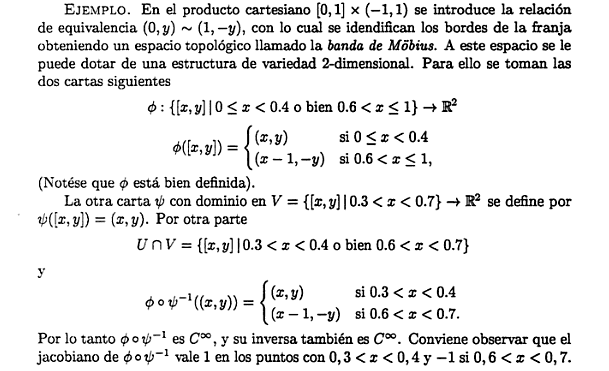
\includegraphics[keepaspectratio=true,width=\linewidth]{img/ejemplo_6.png}
\end{center}

Para dotar a un conjunto de estructura diferencial basta con encontrar un atlas para el cual se cumpla la definición de estructura diferencial sobre el conjunto dado.

Tomamos 8 cartas de la siguiente forma:
\begin{enumerate}
\item
\[\appl{\phi_1}{\{(x,y,z) \tq x\in [0,1), y \in [0,1), z \geq 0\}}{\real^3}\]
siendo $\phi_1=Id$
\item
\[\appl{\phi_2}{\{(x,y,z) \tq x\in (-1,0], y \in [0,1), z \geq 0\}}{\real^3}\]
siendo $\phi_2([x,y,z])=(-x,y,z)$
\item
\[\appl{\phi_3}{\{(x,y,z) \tq x\in [0,1), y \in (-1,0], z \geq 0\}}{\real^3}\]
siendo $\phi_3([x,y,z])=(x,-y,z)$
\item
\[\appl{\phi_4}{\{(x,y,z) \tq x\in [0,1), y \in [0,1), z \leq 0\}}{\real^3}\]
siendo $\phi_4([x,y,z])=(x,y,-z)$
\item
\[\appl{\phi_5}{\{(x,y,z) \tq x\in (-1,0], y \in (-1,0], z \geq 0\}}{\real^3}\]
siendo $\phi_5([x,y,z])=(-x,-y,z)$
\item
\[\appl{\phi_6}{\{(x,y,z) \tq x\in (-1,0], y \in [0,1), z \leq 0\}}{\real^3}\]
siendo $\phi_6([x,y,z])=(-x,y,-z)$
\item
\[\appl{\phi_7}{\{(x,y,z) \tq x\in [0,1), y \in (-1,0], z \leq 0\}}{\real^3}\]
siendo $\phi_7([x,y,z])=(x,-y,-z)$
\item
\[\appl{\phi_8}{\{(x,y,z) \tq x\in (-1,0], y \in (-1,0], z \leq 0\}}{\real^3}\]
siendo $\phi_8([x,y,z])=(-x,-y,-z)$

\end{enumerate}

La combinación de una de estas funciones con la inversa de otra no implicará más que cambios de signo sobre las variables de tal forma que
\[\phi_i\circ \inv{\phi_j}(x,y,z)=(\pm x, \pm y, \pm z)\]

Buscamos que estas combinaciones sean difeomorfismos en el entorno en el que están definidas (la intersección de sus dominios) (\fref{def:VariedadDiferenciable}) y queda claro que estas aplicaciones son $C^{\infty}$ y sus inversas, que son de la misma forma, también. Conviene observar que el jacobiano vale siempre $\pm 1$.

Por ejemplo, $Φ_7\circ Φ_8^{-1} (-x,-y,-z) = Φ_7([x,y,z]) = (x,-y,-z)$ en $U_7 ∩ U_8 = \{(x,y,z) \tq x=0, y∈(-1,0], z≤0\}$.

\doneby{Dejuan}\textcolor{green}{Se lo he mandado así por si se anima a corregirlo.}

\textcolor{blue}{Pedro dice: No creo que esto esté bien. El conjunto cociente que tu estás estudiando agrupa más elementos de los necesarios en una clase. Para ti (1,1,0),(1,1,4),(1,1,x) están en la misma clase de equivalente y no debería ser así}

Para darle una estructura diferencial a $C/\sim$ necesitamos primero definir el conjunto.

\[
C/\sim = \{ [x,y,z] \;/\; x^2 + y^2 = 1 \}\quad \text{ con } \quad [x,y,z] = \{(x,y,z),(-x,-y,-z)\}
\]

Para dotarle de una estructura diferencial necesitamos una topología conexa y Hausdorff además de una familia de funciones $f_{\alpha}$ y abiertos $U_{\alpha}$ con unas ciertas propiedades.


La topología conexa y Hausdorff viene dada por la topología de $\mathbb{R}^3$ inducida en $C$, que es conexa y Hausdorff.


Necesitamos $f_{\alpha}$ inyectiva y $U_{\alpha}$ abierto tal que $\bigcup_{\alpha} f_{\alpha}(U_{\alpha}) = C/\sim$. Para ello definimos:


\[
f:[-1,1]×ℝ \longrightarrow C/\sim \quad \quad f_{\alpha}(x,z) =\left[x,\sqrt{1-x^2},z\right]
\]

tomando la raíz cuadrada positiva para asegurar inyectividad (ya que, como la imagen son clases de equivalencia, $(x,\sqrt{1-x^2},z) = (-x,-\sqrt{1-x^2},-z)$. En este caso $U_{\alpha} = [-1,1]×ℝ$

Tenemos que $f_{\alpha}(U_{\alpha}) = C/\sim$ por lo que no necesitamos más cartas en la estructura diferencial.


La última propiedad requerida es que el cambio de carta sea un difeomorfismo. Aquí, como sólo tenemos una carta, el único cambio de carta posible es la identidad que es un difeomorfismo.


\end{problem}

\begin{problem}[8]
Sea $M$ una variedad diferenciable que puede ser recubierta por dos entornos $V_1, V_2$ tales que la intersección  $V_1 ∩ V_2$ es conexa. Demuestra que $M$ es orientable.

\solution

\doneby{Pedro} \approvedby{Guille}

La definición nos dice que una variedad diferencial es orientable si tiene una estructura diferencial $\{(U_α, f_α)\}$ (conjunto de cartas coordenadas) tal que para cada par $α,β$ con $f_α(U_α)\cap f_β(U_β)\neq \emptyset$, la diferencial del cambio de coordenadas $f^{-1}_β \circ f_α$ tiene determinante positivo.

Este ejercicio está inspirado en \href{http://rinconmatematico.com/foros/index.php?action=printpage;topic=22474.0}{esta página web que esta hosteada en una calculadora y al entrar hay altas probabilidades de que esté sobrecargado el servidor y no te deje}

Vamos a estudiar por tanto el signo de $\det(\Dif(f_β^{-1}○f_α))$. Sabemos que este determinante no puede tener valor 0, pues eso implicaría que el determinante de uno de los difeomorfismos fuese 0, ya que
\[\det (\Dif(f_β^{-1}○f_α)) = \det (\Dif f_β^{-1})\cdot \det(\Dif f_α)\]

Además sabemos que el determinante es una aplicación continua y que está definida sobre un conexo (por hipótesis del enunciado). Por tanto su imagen será un conexo en $\real$ (un intervalo) que no contendrá al 0 por lo que, necesariamente, debe ser positivo o negativo. Es decir, no hay posibilidad de que este determinante cambie de signo en el conjunto en el que estamos trabajando.

Si este determinante es siempre positivo, problema resuelto. No hay nada más que hacer.

Si fuese negativo, componemos la parametrización $f_α$ con la aplicación $\appl{g}{\real^m}{\real^m}$ tal que $g(x_1,...x_m)=(-x_1,x_2,...x_m)$, tomando así una nueva parametrización $f_c = f_α \circ g$.

Es decir, si resulta que las cartas escogidas no nos dan ese determinante positivo, cambiamos $f_α$ por $f_c$, con lo que obtenemos un nuevo atlas (estructura diferenciable) $\{(U_β,f_β),(U_c, f_c)\}$ que cumple la definición de orientable.

Puesto que bastaba con que existiera una estructura diferenciable con estas propiedades, ya lo tenemos demostrado.
\end{problem}

\begin{problem}[9] Demuestra que la esfera $S^n = \set{p ∈ ℝ^{n+1} \tq \md{p} = 1}$ es orientable.
\solution

\doneby{Guille}

Implíctamente nos están dando la esfera inmersa en $ℝ^{n+1}$, así que voy a aprovechar para tratar de demostrar lo siguiente.

\begin{prop} Sea $M$ una variedad diferenciable de $n$ dimensiones, y $\appl{G}{M}{ℝ^{n+1}}$ una aplicación continua que asigne a cada punto un vector normal unitario a $M$, esto es, que $∀p ∈ M$ $\pesc{G(p), v} = 0$ para todo $v ∈ \tgs_p M$. Entonces, $M$ es orientable.
\end{prop}

\begin{proof} Partimos de la definición de orientabilidad de \vref{def:OrientacionCutre}. Tenemos un atlas $\set{(U_i, f_i)}$ no orientable (si fuese orientable ya habríamos acabado y esta demostración sería ridícula). Vamos a construir otro atlas que sí sea orientable.

Para ello, definimos nuevas parametrizaciones de la siguiente forma, dados puntos $\vx^i = (x^i_1, \dotsc x^i_n) ∈ U_i$: \[ \tilde{f}_i(\vx^i) = \begin{cases} f_i(\vx^i) & \text{si } [G(f(\vx^i)), ∂x^i_1, \dotsc, ∂x^i_n)] = 1 \\
f_i(-x^i_1, x^i_2, \dotsc, x^i_n) & \text{si } [G(f(\vx^i)), ∂x^i_1, \dotsc, ∂x^i_n)] = -1 \end{cases} \], donde $[G(f(\vx^i)), ∂x^i_1, \dotsc, ∂x^i_n)]$ vale $1$ si esos vectores dan una orientación compatible con la base canónica de $ℝ^{n+1}$ y $-1$ si no.

Dado que $G$ es continua y no nula, $[G(f(\vx^i)), ∂x^i_1, \dotsc, ∂x^i_n)]$ va a ser siempre constante en una carta, luego las $\tilde{f}_i$ van a definir una estructura diferenciable para $M$ sin problemas.

En esta estructura diferenciable se va a cumplir que $[G(\tilde{f}(\vx^i)), ∂x^i_1, \dotsc, ∂x^i_n)] = [G(\tilde{f}(\vx^j)), ∂x^j_1, \dotsc, ∂x^j_n)] = 1$ para cualquier par de cartas $U_i, U_j$. Esto implica que el determinante del jacobiano del cambio de carta tiene signo positivo, luego efectivamente es orientable\footnote{Muy formal no es esto, la verdad}.
\end{proof}

Con esta proposición hecha, vemos que cada punto $p ∈ S^n$ define un vector normal a esa esfera, luego $G(p) = p$ cumple las condiciones de la proposición anterior, así que $S^n$ es orientable.

\end{problem}

\begin{problem}[10]
Prueba que el plano proyectivo $P^2(\real)$ no es orientable.

\textbf{Indicación}. Prueba que si una variedad diferenciable $M$ es orientable, cualquier conjunto abierto en $M$ es una variedad orientable. Observa que $P^2(\real)$ contiene una cinta de Möbius que no es orientable.

\solution

\doneby{Pedro}

Es sencillo de ver que si tomamos la definición de orientable y nos restringimos a las cartas necesarias para cubrir el abierto que tomemos, mantenemos la definición de orientable.

Puesto que el plano proyectivo contiene una cinta de Möbius es claro que no puede ser orientable.

\end{problem}

\begin{problem}[12]
Un campo de planos en un conjunto abierto $U \subset \real^3$ es una correspondencia $P$ que asocia a cada punto $p \in U$ un plano $P(p)$ que pasa por $p$. El campo $P$ es diferenciable si los coeficientes de la ecuación de $P(p)$ son diferenciables en $p$.

Una superficie integral de $P$ es una superficie $S \subset \real^3$ tal que $\tgs_q S=P(q)$, es decir, en cada punto la superficie es tangente al plano del campo que pasa por ese punto.

Sea ω una 1-forma en $U \subset \real^3$ con $ω(q)\neq 0$, $q \in U$. Prueba que:
\ppart ω define un campo de planos diferenciable $P$ con la condición
\[v \in P(p)\subset \real^3 \iff ω_p(v)=0\]

\ppart Si $S$ es una superficie integral de $P$ que pasa por $p$, entonces $i^*(ω)=0$ donde $\inmr{i}{S}{\real^3}$ es la inmersión de $S$ en $ℝ^3$.

\ppart
Si existe una superficie integral de $P$ que pasa por $p$, para todo $p\in U$ existe una 1-forma σ en un entorno $V \subset U$ de $p$ tal que $\dif ω = ω \y σ$

\textbf{Indicación:} Considera dos 1-formas $ω_2,ω_3$ tales que $ω=ω_1,ω_2,ω_3$ son linearmente independientes en $V$ y escribe:
\[\dif ω = αω_2 \y ω_3 + β ω_3 \y ω_1+γω_1\yω_2\]

Usando el hecho de que $\dif(i^*ω)=i^*\dif ω = 0$ y que la 2-forma $ω_2 \y ω_3$ es distinta de cero, concluye que $α= 0$, luego
\[\dif ω = ω_1 \y (γ ω_2-βω_3)\]

\ppart Si existe una superficie integral de $P$ para todo punto $p \in U$ y $ω=a\dif x + b \dif y + c \dif z$, entonces:
\[\left( \frac{\partial c}{\partial y}-\frac{\partial b}{\partial z} \right)a+\left( \frac{\partial a }{\partial z}-\frac{\partial c}{\partial x} \right)b+\left( \frac{\partial b}{\partial x }-\frac{\partial a}{\partial y} \right)c=0\]

\textbf{Indicación:} Concluye del apartado c) que $\dif ω \y ω = 0$ y escribe esta ecuación en coordenadas.

\solution

\doneby{Pedro} \approvedby{Dejuan} \approvedby{Guille}

\spart

Tomando una $ω=a\dif x + b \dif y + c \dif z$ cualquiera, donde $a,b,c$ son funciones de $(x,y,z)$, el campo de planos asociado estaría formado por aquellos vectores que, en cada punto, cumplen:
\[P(p)=a(p)v_x+b(p)v_y+c(p)v_z=0 \text{ siendo } v_x,v_y,v_z \text{ las coordenadas del vector } v\]

Es decir, el campo de planos sería la aplicación $P$ que dado un punto $p$ nos lleva al plano $P(p)$. Puesto que las funciones $a,b,c$ son diferenciables (pues son los coeficientes de una forma diferencial), es claro que los coeficientes del plano $P(p)$ serán diferenciables.

Por tanto sólo queda comprobar la propiedad de que el plano pasa por el punto $p$. Es decir, queda ver que:
\[a(p)p_x+b(p)p_y+c(p)p_z=0\]

La forma de garantizar esto es trasladando el plano obtenido $P(p)$ para que pase por el punto $p$. Así, nos quedaría la aplicación
\[P(p)=a(p)x+b(p)y+c(p)z-a(p)p_x+b(p)p_y+c(p)p_z=0\]
escrito con la forma habitual de escribir planos que todos conocemos.

\spart
$S$ es una superficie integral de $P$ en $p$, tenemos que $\tgs_p S = P(p)$ que por el apartado anterior, $\tgs_p S = P(p) = \{v ∈ ℝ^3 \tq ω_p(v) = 0\}$.

Pero esta $ω$ está definida en $ℝ^3$ y no en $S$, con lo que lo anterior no es del todo correcto. Lo correcto sería definir $ω$ en $S$ utilizando el pullback de la inclusión. Sea $v∈\tgs_p S$. Entonces

\[
i^*(ω)[v] \overset{1}{=} ω_{i(p)} [\Dif i_p(v)] \overset{2}{=} ω_p [\Dif i_p(v)] \overset{3}{=} 0
\]

\textbf{(1):} Por definición de pullback.

\textbf{(2):} $i(p) = p$ por ser $i$ una inmersión.

\textbf{(3):} Estamos aplicando $ω_p$ a un $v$ que pertenece a $T_pS = P(p)$, ya que $v∈ℝ^3$, $T_pℝ³ = ℝ³$ y la diferencial de $i$ me lo lleva a $v'∈ T_pS$.

Según \href{http://math.stackexchange.com/questions/509603/the-derivative-of-the-inclusion-map-is-the-inclusion-map-of-tangent-spaces}{treble de stackexchange}, si $\inmr{i}{X}{Y}$ es una inclusión, entonces $\appl{\Dif i_p}{\tgs_p X}{\tgs_p Y}$, y como el tangente de $ℝ^3$ es $ℝ^3$ (o algo así dice el doCarmo) $Di_p(v) ∈ \tgs_pS$.

%
%Si atendemos a la construcción de $S$ vemos que, en cada punto $p$, la superficie tendrá como tangente el plano $P(p)$, por lo que, en todo punto, la superficie es perpendicular a $(a(p),b(p),c(p))$. Por tanto, al traer la 1-forma ω de $\real^3$ a la superficie $S$, tendremos que absolutamente todas las evaluaciones posibles de ω en un punto y un vector de $S$ (siendo un vector que pasa por el punto), nos va a dar 0.
%
%Por tanto, la restricción de ω a la superficie integral $S$ es 0.

\spart

Vamos a seguir los pasos dados por la indicación. Definimos dos 1-formas:
\begin{align*}ω_2=a_2\dif x + b_2 \dif y + c_2 \dif z \\ ω_3=a_3\dif x + b_3 \dif y + c_3 \dif z \end{align*}
de forma que sean linealmente independientes y escribimos la ecuación indicada:


\[\dif ω = αω_2 \y ω_3 + β ω_3 \y ω_1+γω_1\yω_2\]

Evidenetemente $ω_2\y ω_3$ no es nula, puesto que son independientes. (Si lo hacemos a mano vemos que el producto equivale a los coeficientes obtenidos al calcular el producto vectorial de los vectores que forman los coeficientes. Si nos sale todo 0 obtenemos que los vectores han de ser proporcionales, y sabemos que no es así por hipótesis de la definciión de estas $ω_2, ω_3$).

Si ahora calculamos $i^*(\dif ω)$, apliando las propiedades del pull back obtenemos:
\[i^*(\dif ω) = αi^*(ω_2) \y i^*(ω_3) + β i^*(ω_3) \y i^*(ω_1)+γi^*(ω_1)\y i^*(ω_2)  \iff 0 = αi^*(ω_2) \y i^*(ω_3)\]
puesto que $ω_1=ω \implies i^*(ω_1)=0$.

Además, tenemos $α=0$ porque
\[
i^*(\dif ω) = \dif (i^* ω) = \dif 0 = 0. \implies αi^*(ω_2) \y i^*(ω_3) = α(i^*(ω_2∧ω_3)) = 0
\]

por ser $ω_2,ω_3$ linealmente independientes.


Así nos queda:
\[\dif ω = ω_1 \y (γω_2-βω_3) = ω \y σ\]
que es justo lo que se nos pedía demostrar.


\spart

Puesto que ya teníamos del apartado anterior $\dif ω = ω_1 \y (γω_2-βω_3) $, multiplicando por ω a ambos lados tenemos:
\[\dif ω \y ω = ω_1 \y (γω_2-βω_3) \y ω = -ω_1 \y ω \y (γω_2-βω_3) =0 \]
puesto que $ω_1 = ω$ y $ω \y ω = 0$ \footnote{$ω$ es una 1-forma y el producto de k-formas impares consigo mismas es 0 (\fref{ej:T1_E4})}.

Ahora vamos a calcular $\dif ω \y ω$ a partir de la ω genérica:
\[\dif ω \y ω =\left( (b_x-a_y)\dif x \dif y + (c_x-a_z)\dif x \dif z + (c_y-b_z)\dif y \dif z \right)ω =\]
\[=\left(c(b_x-a_y)-b(c_x-a_z)\right) +a(c_y-b_z)\dif x \y \dif y \y \dif z=0\]
que es justo lo que se nos pedía demostrar.


\end{problem}

\begin{problem}[13]
Sea $ω=x\dif x + y \dif y + z \dif z$ y sea $P$ el campo de planos en $\real^3 \setminus \{0\}$ determinados por ω. Muestra que la superficie integral de $P$ en el punto $p=(x,y,z)$ es la esfera centrada en el origen que pasa por $p$.

\solution

\doneby{Pedro}

El campo de planos dado sería:
\[P(p)=p_x x + p_y y+p_c z = 0\]
siguiendo la notación de bachillerato para planos.

La superficie integral será tangente en cada punto al plano $P(p)$.

El vector normal de este plano es el vector radio y la superficie que es perpendicular en todo punto al vector radio es la esfera centrada en el origen.

\end{problem}

\begin{problem}[14]
Sea $ω=z\dif x + x \dif y + y \dif z$ y sea $P$ el campo de planos en $\real^3 \setminus \{0\}$ determinados por ω. Muestra que este campo de planos no tiene superficie integral

\solution

\doneby{Dejuan}

\approvedby{Pedro}

El apartado d) del ejercicio 14 nos dice \textit{si existe una superficie integral entonces se cumplen estas ecuaciones}. Si no se cumplieran esas ecuaciones, no podría existir superficie integral. Vamos con el cálculo, teniendo en cuenta que $a=z,b=x,c=y$:

\[\left( \frac{\partial c}{\partial y}-\frac{\partial b}{\partial z} \right)a+\left( \frac{\partial a }{\partial z}-\frac{\partial c}{\partial x} \right)b+\left( \frac{\partial b}{\partial x }-\frac{\partial a}{\partial y} \right)c= (1-0)z + (1-0) x + (1-0) y ≠ 0\]

Concluimos que no puede existir una superficie integral en $ℝ^3$ (solo podría ser que tuviera superficie integral en los puntos tales que $x+y+z=0$)

\doneby{Pedro}

\textcolor{blue}{A continuación voy a tratar de explicar adecuadamente la solución de este ejercicio que hizo el profesor en clase.}

Sea $ω = z \dif x + x \dif y + y \dif z$. Nos piden demostrar que no tiene una superficie integral, que es lo mismo que demostrar que no tiene fórmula integral. La superficie integral es una tal que restringiendo la 1-forma a la ella, obtengamos 0, es decir:
\[\restr{w}{s} = 0 \dimplies ω(D) = 0 \]
con $D∈\tgs S$ un campo tangente.

	Como estamos buscando una superficie, buscamos 2 campos que sean tangentes y que cumplan la condición descrita arriba.

	Observando la forma de ω, podemos ver que
	\[D_1 = x \dpa{}{x} - z\dpa{}{y} \text{ y } D_2 = y\dpa{}{x} - z\dpa{}{z}\]
	son 2 campos que cumplen la condición por construcción.

	La inspiración para llevar a cabo la traducción \textit{Rafael Hernández}-\textit{Castellano} se encuentra \href{http://www.uam.es/personal_pdi/ciencias/fchamizo/asignaturas/mgeom1112/mgeom_2.pdf}{aquí}.

	Una vez que tenemos estos dos campos que cumplen la condición pedida (anulan a la 1-forma), tenemos que ver si existe una superficie que tenga a estos dos campos de vectores como vectores tangentes.

	\obs En definitiva, queremos buscar una superficie que sea tangente en todo punto al campo de planos generado por ω. Hemos encontrado dos campos de vectores que generarían el campo de planos. Ahora tenemos que ver si existe una superficie que siempre sea tangente a ellos o no.

	Aquí es donde entra en juego el \textbf{Teorema de Frobenius}, que nos asegura que una distribución es involutiva si y sólo si es completamente integrable.

	Por definición tenemos que una distribución será involutiva si el corchete de Lie es cerrado en ella, es decir, el corchete de Lie de los dos campos que están en Δ también esta en Δ.

	Sea $M$ una variedad n-dimensional. Una \textbf{distribución} Δ de dimensión $k$ es una forma de asignar a cada punto $p \in M$ un subespacio $k$ dimensional $Δ_p \subset \mathbb{T}_p(M)$, de forma que en un entorno $U(p)$ venga generado por campos de vecotres $\{X_1,...x_k\}$.

	Dada una distribución Δ el análogo de las curvas integrales será ahora una subvariedad cuyo espacio tangente en cada punto coincida con $Δ_p$.

	Aplicando el Teorema de Cartan tenemos que;
	\[\dif \omega(D_1,D_2) = \underset{=0}{D_1\omega(D_2)} - \underset{=0}{D_2ω(D_1)} - ω([D_1,D_2])\]

	Si se cumpliera $[D_1,D_2]∈Δ$, tendríamos que $ω([D_1,D_2]) = 0$, con lo que $\dif ω(D_1,D_2) = 0$. Si vemos que $\dif ω(D_1,D_2) ≠ 0$, entonces tendremos que no tiene fórmula integral, pues la distribución no será involutiva.

	$\dif ω = \dif z \y \dif x + \dif x \y \dif y + \dif y\y \dif z$ Si aplicamos estos 3 sumandos, tendremos:
	\[
	\dif z \y \dif x (D_1,D_2) = \det\begin{pmatrix}
	\dif z(D_1) & \dif x(D_1) \\ \dif z(D_2) & \dif x(D_2)
	\end{pmatrix} = xz
	\]

	Haciendo el cálculo con los otros 2 sumandos de $dω$, obtenemos:

	\[\dif ω(D_1,D_2) = xz + yz + z^2 ≠ 0\]

\end{problem}

\begin{problem}[15] \label{ej:Variedades-15}
Considera en la recta real $\real$ las siguientes dos estructuras diferenciales:
\begin{itemize}
\item $(\real_1, f_1)$ con $f_1(x)=x$
\item $(\real_2, f_2)$ con $f_2(x)=x^3$
\end{itemize}
Demuestra que

\ppart
La identidad $\appl{i}{(\real_1, f_1)}{(\real_2, f_2)}$ no es un difeomorfismo (esto es, las estructuras maximales determinadas por ambas estucturas son distintas).

\ppart
La aplicación $\appl{\phi}{(\real_1, f_1)}{(\real_2, f_2)}$ dada por $\phi(x)=x^3$ es un difeomorfismo (esto es, aunque las estructuras diferenciales son distintas, definen variedades diferenciales difeomorfas).

\solution

\doneby{Guille}

\begin{figure}[hbtp]
\centering
\inputtikz{E_IV_DifeomorfismoRectaReal}
\caption{Esquema de los posibles difeomorfismos entre dos estructuras diferenciales de la recta real.}
\label{fig:DifeomorfismoRectaReal}
\end{figure}

Queremos ver que la aplicación que nos lleva de una variedad a la otra (entendiendo como variedad cada una de las dos estructuras diferenciables de $ℝ$, ver \fref{fig:DifeomorfismoRectaReal}) es un difeomorfismo. Para ello tiene que ser función diferenciable compatible con las cartas (ver \fref{def:FuncionDiferenciableVariedades}). Vamos a ello.

\spart

La aplicación que nos mueve entre cartas es $f_1 ○ i ○ \inv{f_2} = \sqrt[3]{x}$, que no es diferenciable con $x = 0$, por lo tanto no es un difeomorfismo.

\spart

En este caso, la aplicación que nos lleva de una carta a otra es $f_1 ○ \phi ○ \inv{f_2} = x$ que claramente es un difeomorfismo.

\end{problem}

\begin{problem}[16] Sea $M$ una variedad diferenciable conexa. Para cada $p ∈ M$, definimos por $\mathcal{O}_p$ el espacio cociente de todas las bases de $\tgs_p M$ bajo la siguiente relación de equivalencia: dos bases son equivalentes si están relacionadas por una matriz con determinante positivo. Claramente $\mathcal{O}_p$ tiene dos elementos, y cada elemento $O_p$ de $\mathcal{O}_p$ será una orientación en $p$. Ahora, sea \[ \tilde{M} = \set{(p, O_p) \tq p ∈ M, O_p ∈ \mathcal{O}_p } \] y sea $\appl{f_α}{U_α}{M}$ una parametrización de $M$ con $p ∈ f_α(U_α)$. Definimos $\appl{\tilde{f}_α}{U_α}{\tilde{M}}$ de la siguiente forma:
\[ \tilde{f}_α(x_1, \dotsc, x_n) = \left((f_α(x_1, \dotsc, x_n), \left[∂x_1, \dotsc, ∂x_n \right]\right)\]
donde $(x_1, \dotsc, x_n) ∈ U_α$ y $\left[∂x_1, \dotsc, ∂x_n \right]$ denota el elemento de $\mathcal{O}_p$ dado por esta base. Demuestra que

\ppart Si $\set{(U_α, f_α)}$ es una estructura diferenciable en $M$, entonces $\set{(U_α, \tilde{f}_α)}$ lo es también en $\tilde{M}$ y que además es orientable, incluso cuando $M$ no lo es.

\ppart La aplicación $\appl{π}{\tilde{M}}{M}$ dada por $π(p, O_p) = p$ es diferenciable, sobreyectiva, y cada punto $p ∈ M$ tiene un entorno $V$ cuya imagen inversa $\inv{π}(V)$ es la unión disjunta de dos conjuntos abiertos, cada uno de los cuales es difeomorfo con $V$ por π. Por esta razón, a $\tilde{M}$ se le llama la cobertura doble orientable de $M$.

\ppart $M$ es orientable si y sólo si $\tilde{M}$ no es conexo.

\textit{Sugerencia}: Si $M$ es orientable, los conjuntos $M_1 = \set{(p, O^1_p)}$ y $M_2 = \set{(p, O^2_p)}$ con $O^1_p, O^2_p$ orientaciones opuestas de $M$ en $p$, son ambos subconjuntos de $\tilde{M}$ no vacíos, disjuntos y abiertos. Para la implicación contraria, hay que demostrar primero que la imagen $π(F)$ de un conjunto cerrado $π ⊆ \tilde{M}$ es un conjunto cerrado en $M$: esto viene dado por el hecho de que para cada $p ∈M$ la imagen inversa $\inv{π}(p)$ tiene dos puntos. Ahora, si $\tilde{M}$ no es conexo, denotamos por $C$ una componente conexa de $\tilde{M}$. Entonces $π(C)$ es un subconjunto abierto, cerrado y no vacío de $M$, luego $π(C) = M$. Entonces, $\tilde{M}$ es la unión disjunta de dos componentes conexas y $π$ aplica difeomorfamente cada componente en $M$. Sigue que $M$ es orientable.

\solution

\doneby{Guille}

\spart

Esta parte no es demasiado difícil de ver. Para estudiar la orientabilidad de $\tilde{M}$, vemos qué ocurre en los cambios de carta. Tomemos dos cartas $U_i, U_j ⊂ \tilde{M}$ con $\tilde{f}_i(U_i) ∩ \tilde{f}_j(U_j) ≠ ∅$, y con coordenadas $x_1, \dotsc, x_n$ y $y_1, \dotsc, y_n$ en cada carta respectivamente. Como la intersección de sus imágenes no es vacía, tiene que ser por fuerza $[∂x_1, \dotsc, ∂x_n] = [∂y_1, \dotsc, ∂y_n]$, luego ambas cartas tienen orientaciones compatibles.

Otra manera de verlo es que si tenemos dos cartas $U_i, U_j$ que intersecan en $M$ (esto es, $f_i(U_i) ∩ f_j(U_j) ≠ ∅$) con orientaciones incompatibles, entonces esas dos cartas no van a intersecar en $\tilde{M}$ porque $[∂x_1, \dotsc, ∂x_n] ≠ [∂y_1, \dotsc, ∂y_n]$. Es decir, que incluso cuando $M$ no es orientable, $\tilde{M}$ sí puede serlo.

\spart

Que es sobreyectiva se ve fácilmente, y que es diferenciable también por ser la identidad en una componente (el punto en $M$). También es fácil ver que $\inv{π}(V)$ es la unión disjunta de dos conjuntos abiertos: uno con los puntos de $V$ con una orientación y otro con los mismos puntos pero con orientación contraria. Además, al llevar cada punto en sí mismo, está claro que cada uno de esos abiertos será difeomorfo con $V$.

\spart
\end{problem}

\section{Integración en variedades}

La teoría de estos ejercicios de \cite[Capítulo 4]{doCarmo94} está en el \fref{chap:Integracion}.

\begin{problem}[2]
\ppart Sea $ω = x \dif y - y \dif x$ y $\inmr{j}{M}{ℝ^2}$ la inmersión de una región con borde $∂M$. Demuestra que el área de $M$ viene dada por \[ \mop{\acute{A}rea} M = \frac{1}{2} \int_{∂M} j^* ω \]

\ppart Sea $ω = x \dif y \y \dif z - y \dif x \y \dif z + z \dif x \y \dif y$ y $\inmr{j}{M}{ℝ^3}$ la inmersión de una región con borde regular $∂M$. Demuestra que el volumen de $M$ viene dado por \[ \mop{Vol} M = \frac{1}{3} \int_{∂M} j^* ω \]

\ppart Generaliza estos resultados para $ℝ^n$.
\solution
\doneby{Guille}

\spart Sabemos que el área de la variedad viene dada por la integral de la 2-forma constante $1$ sobre toda la variedad, esto es, \[ \mop{\acute{A}rea} M = \int_M 1 \df{x,y}\]

¿Qué ocurre si calculamos la diferencial de ω? Tenemos que \[ \dif ω = \dif x \y \dif y - \dif y \y \dif x = 2 \dif x \y \dif y \], es decir, 2 veces la 2-forma constante 1. Así, podemos pasar de la integral en toda la variedad a la integral en el borde a través de Stokes (\fref{thm:Stokes}) y nos queda que \[ \frac{1}{2} \int_{∂M} j^* ω \eqexpl{Stokes} \frac{1}{2} \int_M \dif ω = \frac{1}{2} \int_M 2 \dif x \y \dif y = \int_M \dif x \y \dif y = \mop{\acute{A}rea} M \]

\spart No es muy difícil volver a seguir el procedimiento de antes para ver que $\dif ω = 3 \dif x \y \dif y \y \dif z$ haciendo los cambios de signo correspondientes. Igual que antes, el volumen será la integral de la 3-forma constante $1$ sobre toda la variedad, así que por Stokes podremos convertir la integral sobre el borde a una integral de $\dif ω$ sobre la variedad y tendremos el resultado de nuevo.

\spart Parece claro que el resultado va a salir para todos los casos. La cuestión es formalizarlo bien, sobre todo la forma diferencial esa.

Sean $x_1, \dotsc, x_n$ las coordenadas de $ℝ^n$. Entonces definimos \[ ω = \sum_{i=1}^n \left((-1)^{i-1} x_i \bigwedge_{\substack{k = 1 \\ k ≠ i}}^n \dif x_k \right)\], poniendo ese $(-1)^{i-1}$ para compensar los cambios de signo que tendremos que hacer al sacar la diferencial

Obtenemos ahora su diferencial exterior, y nos queda que \[ \dif ω = \sum_{i=1}^n \left((-1)^{i-1} \dif x_i \bigwedge_{\substack{k = 1 \\ k ≠ i}}^n \dif x_k \right) = \sum_{i=1}^n \bigwedge_{k=1}^n \dif x_k = n \dif x_1 \y \dotsb \y \dif x_n \]

Ahora podemos aplicar Stokes. Sabemos que el volumen (o como quiera que se llame el mismo concepto para variedades $n$-dimensionales) viene dado por la integral de la $n$-forma constante $1$ sobre toda la variedad, así que \[ \frac{1}{n} \int_{∂M} j^* ω \eqexpl{Stokes} \frac{1}{n} \int_M \dif ω = \int_M \dif x_1 \y \dotsb \y \dif x_n = \mop{Hipervol.} M \]

\end{problem}

\begin{problem}[7]
Sean $ω_1, ω_2$ formas diferenciales en una variedad diferenciable $M$. Supongamos que ambas son cerradas y que $ω_2$ es exacta. Demuestra que $ω_1 \y ω_2$ es cerrada y exacta.

\solution

\doneby{Guille}

Una forma $ω$ es cerrada (\fref{def:FormaCerrada}) si $\dif ω = 0$, y es exacta (\fref{def:FormaExacta}) si existe otra forma $α$ tal que $\dif α = ω$. Luego lo que tenemos es que $\dif ω_1 = \dif ω_2 = 0$ y que además existe $α$ tal que $\dif α = ω_2$.

Vamos a ver primero si $ω_1 ∧ ω_2$ es cerrada. Calculamos su diferencial y vemos que \[ \dif(ω_1∧ω_2) = \dif ω_1 ∧ ω_2 \pm ω_1 ∧ \dif ω_2 = 0 \] ya que ambas son cerradas, luego $ω_1 ∧ ω_2$ es cerrada.

Fijándonos en la definición de la diferencial del producto exterior, podemos calcular \[ \dif(ω_1∧α) = \dif ω_1 ∧ α + (-1)^p ω_1 ∧ \dif α = (-1)^p ω_1 \y ω_2 \], con $p$ el grado de α. Si $p$ es impar y nos sale un signo negativo, simplemente cogemos $- ω_1 ∧ α$ para que nos dé $\dif(-ω_1 ∧ α) = ω_1 \y ω_2$.
\end{problem}

\begin{problem}[8] \label{ej:Integracion-8}
Sea $M^n$ una variedad orientable compacta sin borde, y sea ω una $(n-1)$-forma diferenciable en $M^n$. Demuestra que existe un punto $p∈M$ tal que $(\dif ω)_p = 0$.
\solution

\doneby{Edu}

\approvedby{Pedro}

Sea $i:\partial M \hookrightarrow M$ inmersión. Entonces, por tratarse de una variedad sin borde:
\[ \int_{\partial M} i^* \omega = \int_{\emptyset} i^* \omega = 0\]

Luego, como debería cumplirse el Teorema de Stokes:
\[ 0 = \int_{\partial M} \omega = \int_{M} \dif \omega \implies \dif \omega = 0 \ \text{ para algún } p \in M \]
{\bf Razón:}
Para que la integral dé 0, hay dos casos:
\begin{itemize}
	\item $\dif \omega$ constantemente 0.
	\item $\dif \omega$ toma valores positivos y negativos, que hacen que esas partes de la integral se cancelen. Al tomar las cartas de M, si en unas es negativa y en otras positiva, por Bolzano en algún punto de las intersecciones se tiene que anular; y lo mismo ocurre si en una misma carta toma valores negativos y positivos.
\end{itemize}

\end{problem}

\begin{problem}[9] Demuestra que no existe ninguna inmersión $\appl{f}{\crc}{ℝ}$ de la circunferencia unidad en la recta real $ℝ$.

\textit{Sugerencia}: Utiliza el \fref{ej:Integracion-8}.
\solution

\doneby{Guille}

\approvedby{Pedro}

\textcolor{blue}{He quitado eso de que $f^*(ω)$ es constante por que no me gustaba nada.}

Vamos a definir $ω = x$ como una $0$-forma en $ℝ$ (tomando como coordenada $x$). En ese caso, $\dif ω = \dif x ≠ 0$ para todo punto de $ℝ$. Por las propiedades del pull back sabemos que $f^*(\dif ω ) \neq 0$.

Ahora bien, $f^*(\dif ω) = \dif (f^*ω)$, que es una $1$-forma diferenciable en $\crc$, y por el \fref{ej:Integracion-8} tiene que existir un punto $p ∈ \crc$ tal que $(\dif (f^*ω))_p = 0$, contradicción porque antes habíamos dicho que $\dif(f^*\dif ω)$ era distinto de cero.

\end{problem}

\begin{problem}[12] \label{ej:Integracion-12}
Sea $M^n$ una variedad diferenciable compacta sin borde. Demuestra que $M$ es orientable si y sólo si existe una $n$-forma diferencial ω definida en $M$ que no es nula en ningún punto.

\textit{Sugerencia}: Para demostrar que esto ocurre ``sólo si'', usa una partición de la unidad para construir una $n$-forma no nula definida globalmente en $M$.
\solution

Esto está hecho en la demostración de la \fref{prop:EquivalenciaOrientacion}.

\doneby{Pedro}

Tenemos que demostrar los dos sentidos de la implicación.

\begin{itemize}
\item \textbf{Sabiendo que $M^n$ es orientable demostramos la existencia de ω}

Una n-forma, ω, que no se anula en una carta es $ω_i = \dif x_1 \y ... \y \dif x_n$ donde $x_i$ son las coordenadas de la carta $U_i$. Ahora extendemos esta forma para que este definida en todo $M^n$ con ayuda de las particiones de la unidad:
\[ω = \sum ρ_i ω_i\]

Ahora tenemos que probar que $ω_x \neq 0 \ \forall x \in M^n$. Cuando este punto $x$ sólo pertenezca a una carta tendremos $ω_x = \dif x_1 \y ... \y \dif x_n$, que evidentemente es distinto de 0.

La dificultad se encuentra en aquellos puntos $x$ que pertenecen a varias cartas. En estos casos tendremos
\[ω = ρ_1(\dif x_{1_1} \y ... \y \dif x_{1_n})+ρ_2(\dif x_{2_1} \y ... \y \dif x_{2_n})+...\]
donde tendremos diferentes diferenciales según la carta en que nos encontremos.

Para poder trabajar con esto tendremos que movernos a la representación de una de esas cartas. Sin pérdida de generalidad, supongamos que $x\in U_1$ y sea $J_i$ el Jacobiano del cambio de carta de $U_i$ a $U_1$. Así nos queda
\[ω = ρ_1(\dif x_1 \y ... \y \dif x_n)+ρ_2J_2(\dif x_1 \y ... \y \dif x_n)+...\]

puesto que los Jacobianos son positivos, por ser la superfice orientable, y los $ρ_i>0$ por definición, queda claro que ω será distinta de 0.

\item \textbf{Sabiendo que existe ω demostramos que $M^n$ es orientable}

En esta ocasión tenemos la variedad $M^n$ n-dimensional y una n-forma ω que no se anula en ningún punto de $M^n$. Tomemos un entorno $U$ de $x\in M^n$ y definimos la función $\appl{α_x}{U}{\real^n}$, que es un difeomorfismo sobre su imagen.

Entonces tenemos que
\[(α_x^{-1})^* ω = f \dif x_1 \y ... \y \dif x_n\]
con $f$ definida en un abierto de $\real^n$ y positiva.

Básicamente estamos tomando la inversa de $α_x$ que es una aplicación que va de $\real^n$ a la variedad que estamos trabajando y calculando el pull back de nuestra forma ω. Por tanto, obtenemos una forma definida en $\real^n$.

A partir de las inversas de los $α_x$ podemos obtener un atlas para $X$. Sean $α_i,α_j$ dos difeomorfismos que se intersecan tenemos:
\[(α_i^{-1})^* ω = f \dif x_1 \y ... \y \dif x_n\]
\[(α_j^{-1})^* ω = g \dif y_1 \y ... \y \dif y_n\]

Ahora sólo tenemos que escribir la diferencial $\dif y_1 \y ... \y \dif y_n$ en función de las variables $x_i$, obteniendo:
\[g(y_i(x_1,...,x_n),...)\text{det}\left(\frac{\partial y_i}{ \partial x_j}\right)_{i,j}\dif x_1 \y ... \y \dif x_n = f(x_1,...x_n)\dif x_1 \y ... \y \dif x_n\]

Como suponíamos $f,g$ positivas, el determinante del Jacobiano ha de ser positivo y por tanto la superfice es orientable.

\end{itemize}

\end{problem}

\begin{problem}[13] Sea $M$ una variedad diferenciable compacta y orientable sin borde. Demuestra que $M$ no se puede contraer a un punto.

\textit{Sugerencia}: Utiliza el \fref{ej:Integracion-12}, el \nref{lem:Poincare} y el \nref{thm:Stokes}.
\solution

\doneby{Guille}

\approvedby{Pedro}

Hagámoslo por reducción al absurdo y supongamos que sí se puede contraer a un punto.

Por el \fref{ej:Integracion-12} y por ser $M$ compacta y orientable, existe una $n$-forma ω que no se anula en ningún punto de $M$. Como es una $n$-forma, está claro que\footnote{No tenemos más variables, al sacar la diferencial repetiremos diferenciales y el producto exterior de diferenciales repetidas es 0.} $\dif ω = 0$.

Si $M$ se puede contraer a un punto, entonces cualquier abierto es contractible y podemos aplicar el \nref{lem:Poincare}, que nos dice que en este caso cualquier forma cerrada es exacta (y viceversa). Como acabamos de decir que $\dif ω = 0$, entonces ω es cerrada, luego también es exacta por Poincaré y entonces existirá una $(n-1)$-forma α tal que $\dif α = ω$.

Vamos a probar a integrar entonces $ω = \dif α$ sobre la variedad. Usando Stokes, tenemos que \[ I = \int_X ω \eqexpl{Poincaré} \int_X \dif α \eqexpl{Stokes} \int_{∂X} i^* α \]

Ahora bien, como $M$ no tiene borde ($∂X = ∅$), la integral $I$ sólo puede ser 0, luego es obligatorio que $\int_X ω = 0$. Pero $X$ no es vacío, así que lo único que nos queda es que en algún momento esa integral de ω se anule. Esto no puede ocurrir porque habíamos dicho que ω no se anulaba en ningún punto, sólo puede ser positiva o negativa, y es imposible entonces que esa integral se anule. Contradicción, por lo que $M$ no se puede contraer a un punto.

\end{problem}

\begin{problem}[14]
Sean $A,B,C$ funciones diferenciables en $ℝ^3$. Consideramos el siguiente sistema de ecuaciones diferenciales \begin{align*}
A &= \dpa{R}{y} - \dpa{Q}{z} \\
B &= \dpa{P}{z} - \dpa{R}{x} \\
C &= \dpa{Q}{x} - \dpa{P}{y}
\end{align*} donde $P,Q,R$ son funciones desconocidas en $ℝ^3$.

\ppart Demuestra que \[ \dpa{A}{x} + \dpa{B}{y} + \dpa{C}{z} = 0\] es condición necesaria y suficiente para que exista una solución.

\textit{Sugerencia}: Considera la forma diferencial en $ℝ^3$ dada por \[ ω = A \dif y \y \dif z + B \dif z \y \dif x + C \dif x \y \dif y\] y calcula su diferencial exterior. Por el lema de Poincaré, $\dif ω = 0$ si y sólo si existe una forma $α = P\dif x + Q \dif y + R \dif z$ con $\dif α = ω$, esta última condición es precisamente el sistema anterior.

\ppart Supongamos que la condición anterior se satisface y determina las funciones $P,Q,R$.

\textit{Sugerencia}: Considera la contración $H(p,t) = tp$ de $ℝ^3$  a $(0,0,0)$. Entonces \[ \gor{ω} = H^*ω = A(tx,ty,tz)(y t \dif t \y \dif z - zt \dif t \y \dif y) + \dotsb + \text{términos sin } \dif t \]

Así la forma α del apartado anterior vendría dada por \[ α = I \gor{ω} = \left(\int_0^1 A(tx,ty,tz) t \dif t\right)(y\dif z - z \dif y) + \dotsb \]
\solution

\spart
\doneby{Guille}

Hacemos caso de la sugerencia y calculamos esa diferencial (voy a usar la notación $\dpa{A}{x} \equiv A_x$ porque no me apetece escribir):
\begin{multline*}
\dif ω = A_x \dif x ∧ \dif y ∧ \dif z + B_y \dif y ∧ \dif z ∧ \dif x + C_z \dif z ∧ \dif x ∧ \dif y = \\
= \left( A_x + B_y + C_z \right) \dif x ∧ \dif y ∧ \dif z
\end{multline*}

Por lo tanto, decir que $\dif ω = 0$ es lo mismo que decir que se cumple la condición del apartado. Calculamos ahora la diferencial del $α$ que nos dan y vemos que \begin{multline*}
\dif α = P_y \dif y ∧ \dif x + P_z \dif z \y \dif x + Q_x \dif x ∧ \dif y + Q_z \dif z ∧ \dif y + R_x \dif x ∧ \dif z + R_y \dif y ∧ \dif z = \\
= (R_y - Q_z) \dif y ∧ \dif z + (P_z -R_x) \dif z ∧ \dif x + (Q_z - P_y) \dif x ∧ \dif y
\end{multline*}

Si igualamos coordenada a coordenada, tenemos efectivamente el sistema que nos daban. Como en $ℝ^3$ podemos aplicar Poincaré sin ningún problema, tenemos que $\dif ω = 0 \iff \dif α = ω$, que es lo que nos pedían.

\spart
\doneby{Pedro}

Ahora suponemos que se cumple la condición anterior y por tanto el sistema tiene solución. En estas condiciones tenemos que calcular $P,Q,R$.

Atendiendo a la sugerencia del enunciado consideramos la contracción:
\[H(p,t)=tp \text{ tal que } H(0,p)=0 \ \; \; H(1,p)=p\]
que nos lleva $\real^3$ al origen.

Definimos ahora:
\[\overline{ω}=H^*ω=A(tp) (t \dif x + x \dif t)+ B(tp)(t \dif y + y \dif t)+\]
\[+C(tp)(t \dif z + z \dif t)\]

Para hacer escribir este pull back simplemente hemos aplicado la definición de este, considerando:
\begin{align*}x=tx \implies& \dif x = t \dif x + x \dif t \\ y = ty \implies& \dif y = y \dif t + y \dif y \\ z=tz \implies& \dif z = t \dif z + z \dif t \end{align*}

Y reordenando la fórmula de $\overline{ω}$ que hemos escrito obtenemos exactamente la que nos da el enunciado.

Como asumimos que se satisfacen las condiciones del apartado a), sabemos que ω es exacta y que existe una forma α tal que $\dif α = ω$.

Consideraos ahora $F(x,y,z)=K(H^*ω(x,y,z))$ siendo $K$ una función que vimos en teoría $\appl{K}{Ω^{p+1}(U')}{Ω^p(U)}$ de la siguiente forma: si $ω = a_I \dif x_I$, sin que aparezca la $t$, definimos $K(a_I \dif x_I) ≝ 0$ ya que en la derecha tengo $p$ diferenciales y no hay otra forma de quitar una.

Cuando $ω = a_I(t,x) \dif t \y dif x_I$, entonces $K(ω) ≝ \left(\int_0^1 a_I(t,x) \dif t\right) \dif x_I $. Los elementos son suma de estos dos tipos y como es lineal con definirlo en los ya se queda definido.

Por tanto sólo interesarán los términos $x \dif t, y \dif t, z \dif t$: los otros no tienen $\dif t$ y por $K$ se irán a cero de cabeza. Consideramos ahora $F(x,y,z) ≝ K(Φ^*ω(x,y,z))$, y vemos que nos queda \[ F(x,y,z) = x \int_0^1 P(tx,ty,tx) \dif t +  y \int_0^1 Q(tx,ty,tx) \dif t +  z \int_0^1 R(tx,ty,tx) \dif t \]

Y si derivamos $F$ podemos ver que coincide con $ω$ por lo que podemos deducir las identidades que pide demostrar el enunciado.
%\[\overline{\dif α}=H^*(\dif α)=\dif H^*(α)=\dif \left(P(tp)(t \dif x + x \dif t)+Q(tp)(y \dif t + y \dif y)+R(tp)(t \dif z + z \dif t)\right)=\]
%\[\frac{\partial  (P(tp) \cdot t )}{\partial t}\dif t \y \dif x\]
%\[= tP_x(tp)x\dif x \y \dif t +P(tp)\dif x \y \dif t+tP_y(tp) (\dif y \y \dif x + x\dif y \y \dif t)+tP_z(tp)(t \dif z \y \dif x +x \dif z \y \dif t)+...\]
%Para completar la igualdad deberíamos realizar las mismas operaciones con las otras dos funciones, $Q$ y $R$.

%Trabajando sólo con la parte relativa a $P$, la que hemos escrito, podemos ver que:
%\[\overline{\dif α}=t \frac{\partial P }{\partial t}+\]

%Y seguimos manteniendo la relación:
%\[\dif \overline{α} = \overline{w}\]

 %Para calcularla tenemos que integrar $\overline{ω}$.

%\[α = I\overline{ω}=\left( \int_0^1 A(tx,ty,tz)t\dif t\right)(y\dif z - z \dif y)+\]
\end{problem}

\begin{problem}[16]\textit{(Teorema del punto fijo de Brouwer)}.

\ppart Sea $M^n$ una variedad diferenciable compacta y orientable con borde $∂M ≠ ∅$. Demuestra que no existe ninguna aplicación diferenciable $\appl{f}{M}{∂M}$ tal que la restricción $\restr{f}{∂M}$ sea la identidad.

\textit{Sugerencia}: Supongamos que $f$ existe, y sea ω la $(n-1)$-forma en $∂M$ definida en el \fref{ej:Integracion-12}. Claramente $\dif(f^*ω) = f^*(\dif ω) = 0$, y por lo tanto \[ 0 = \int_M \dif(f^*ω) = \int_{∂M} i^* f^* ω = \int_{∂M} ω ≠ 0\], lo que sería una contradicción.

\ppart Demuestra el teorema del punto fijo de Brouwer: sea $B⊂ℝ^n$ la bola de radio 1. Toda aplicación diferenciable $\appl{g}{B}{B}$ tiene un punto fijo, esto es, existe $q∈B$ tal que $g(q) = q$.

\textit{Sugerencia}: Si $g(p) ≠ p$ para todo $p∈B$, el medio segmento que empieza en $g(p)$ y acaba en $p$ interseca $∂B$ en un punto único, digamos $q = f(p)$. Esta aplicación $\appl{f}{B}{∂B}$ así definida satisface las condiciones del apartado anterior y lleva a una contradicción.

\solution

\doneby{Guille}

\spart

No hay mucho que hacer porque la sugerencia nos da prácticamente todo. Simplemente tenemos que fijarnos en que, si $∂M$ es una variedad de dimensión $n-1$, la diferencial de una $n-1$ forma nos dará cero. Simplemente integrando ω en el borde y usando Stokes nos salen las igualdades de la sugerencia suponiendo que $f$ es la identidad en $∂M$.

\spart

\doneby{Pedro}

Vamos a seguir los pasos de la sugerencia haciendo ver que ha sido idea nuestra llevarlos a cabo.

Vamos a demostrar lo que nos piden por reducción al absurdo. Supongamos pues que no existe punto fijo, de modo que $g(p)\neq p \ \ \forall p \in B$.

En ese caso, podemos unir $p$ con $g(p)$ y prolongar el segmento hasta que interseque $\partial B$ en el punto $q=f(p)$ siendo $\appl{f}{B}{\partial B}$. Esta aplicación sería perfectamente continua y diferenciable por construcción. (ya vimos algo similar a esto en Topología)

El apartado anterior nos garantiza que no existe esta $f$ por lo que la construcción que nos llevó a ella hace aguas por algún sitio. Evidentemente el fallo es considerar que no hay punto fijo.

Queda claro por tanto que sí que tenemos el punto fijo.

\end{problem}


\begin{problem}[0] \label{ej:EnunciadoRafa} \textit{Enunciado por el profesor en clase.} Consideramos $\bbs^3 ⊂ ℝ^4$ la esfera de radio $\sqrt{2}$, y el toro \[ T_2 = \set{(x,y,z,t) \tq x^2+y^2 = 1,\; z^2 + t^2 = 1}\] que está contenido en $\bbs^3$.

\ppart Demostrar que $\bbs^3 \setminus T_2$ es la unión disjunta de dos componentes conexas.
\ppart Sea $ω_3$ la 3-forma dada por \[ ω_3 = z \dif x \y \dif y \y \dif t - x \dif y \y \dif z \y \dif t \]

Calcular la integral de $i^*ω$ en cada una de las componentes conexas calculadas en el apartado anterior.

Esto se puede hacer usando Stokes y sin ello. Se pide hacerlo de las dos maneras.
\solution

\doneby{Guille}

\spart

Vamos a hacer un poquillo de topología. Sea $\rel$ una relación de equivalencia en $\bbs^3 \setminus T_2$ de la siguiente forma: dados $\vx, \vy ∈ \bbs^3 \setminus T_2$, $\vx \rel \vy$ si y sólo si existe una aplicación $\appl{γ}{I}{\bbs^3 \setminus T_2}$ continua tal que $γ(0) = \vx$ y $γ(1) = \vy$. Entonces las clases de equivalencia $\quot{\bbs^3 \setminus T_2}{\rel}$ son las componentes conexas. Esto no es nada nuevo y es simplemnete la relación de equivalencia que usábamos en topología para ver conexión.

Si $\va = (x,y,z,t) ∈ \bbs^3 \setminus T_2$, tiene que ser $x^2 + y^2 ≠ 1$ y/o $z^2 + t^2 ≠ 1$. Ahora bien, por ser $\va ∈ \bbs^3$, se tiene que cumplir que $x^2 + y^2 + z^2 + t^2 = 2$, así que podemos decir que $x^2 + y^2 = 2 - z^2 - t^2$, con la condición de que $x^2 + y^2 ≠ 1$ (en ese caso nos encontraríamos en $T_2$).

Esta ecuación nos divide $\bbs^3$ en dos partes: por un lado, cuando $x^2 + y^2 > 1$ y por otro cuando $x^2 + y^2 < 1$. No es difícil ver que si tenemos dos puntos $(x_0, y_0, z_0, t_0)$ y $(x_1, y_1, z_1, t_1)$ con $\sign(x_0^2 + y_0^2 - 1) = \sign(x_1^2 + y_1^2 - 1)$, entonces podemos encontrar la aplicación γ de la relación de antes que simplemente vaya por geodésicas que mantenga en todo punto el mismo signo de $x^2 + y^2 - 1$. Lo que pasa es que estamos en $ℝ^4$ y no me apetece mucho ponerme a sacar la ecuación de la esfera de radio $\sqrt{2}$ en coordenadas cuatroesféricas para demostrar que esa ecuación existe así que me vais a tener que creer.

\spart

Vamos a hacerlo con Stokes. Calculamos la diferencial de la 3-forma \[ \dif ω_3 = \dif z ∧ \dif x ∧ \dif y ∧ \dif t - \dif x ∧ \dif y ∧ \dif z ∧ \dif t = 0 \], por lo que pasan cosas.


\end{problem}


%%%%%%%%%%%%%%%%%%%%%%%%%%%%%%%%%%%%%%%%%%%%%%%%%%%%%%%%%%%%%%%%%%%%%%%%%%%%%%%%%%%%%%%%%%%%%%%%%%%%
%%%%%%%%%%%%%%%%%%%%%%%%%%%%%%%%%%%%%%%%%%%%%%%%%%%%%%%%%%%%%%%%%%%%%%%%%%%%%%%%%%%%%%%%%%%%%%%%%%%%
%%%%%%%%%%%%%%%%%%%%%%%%%%%%%%%%%%%%%%%%%%%%%%%%%%%%%%%%%%%%%%%%%%%%%%%%%%%%%%%%%%%%%%%%%%%%%%%%%%%%
%%%%%%%%%%%%%%%%%%%%%%%%%%%%%%%%%%%%%%%%%%%%%%%%%%%%%%%%%%%%%%%%%%%%%%%%%%%%%%%%%%%%%%%%%%%%%%%%%%%%
%%%%%%%%%%%%%%%%%%%%%%%%%%%%%%%%%%%%%%%%%%%%%%%%%%%%%%%%%%%%%%%%%%%%%%%%%%%%%%%%%%%%%%%%%%%%%%%%%%%%

\section{Geometría de superficies}

Ejercicios correspondientes a \cite[Capítulo 5]{doCarmo94}, teoría en los capítulos \ref{chap:GaussBonnet} y \ref{chap:GeometriaRiemman}.

\begin{problem}[1] \label{ej:Superficies-1}
Este es un ejercicio sobre el ``toro plano''. Sea $\appl{f}{ℝ^2}{ℝ^4}$ dada por \[ f(x,y) = (\cos x, \sin x, \cos y, \sin y) \] para $(x,y) ∈ ℝ^2$. Demuestra que

\ppart $f$ es una inmersión y $f(ℝ^2)$ es homeomorfo a un toro.
\ppart La referencia dada por $e_1 = \dpa{f}{x}$, $e_2 = \dpa{f}{y}$ en $f(ℝ^2) ⊂ ℝ^4$ es ortonormal en la métrica de $f(ℝ^2)$ inducida por $ℝ^4$. Calcula las formas de las ecuaciones de estructura $ω_1, ω_2, ω_{12}$.
\ppart La curvatura gaussiana de la métrica inducida es idénticamente cero.

\solution

\doneby{Guille}

\spart

Para demostrar que $f$ es una \nlref{def:Inmersion}, tenemos que demostrar que la diferencial $F_{*,p} \equiv \Dif f$ es inyectiva o, en otras palabras, que tiene rango máximo. Vamos a ello: \[ \Dif f = \begin{pmatrix}
-\sin x & \cos x & 0 & 0 \\
0 & 0 & -\sin y & \cos y
\end{pmatrix}\]

Está claro que $\Dif f$ tiene rango máximo (el seno y el coseno no van a ser 0 a la vez) y por lo tanto $\Dif f$ es inyectiva, y $f$ es una inmersión.

Para demostrar $f(ℝ^2)$ es homeomorfo a un toro, tenemos que encontrar un \nlref{def:Homeomorfismo} de $f(ℝ^2)$ al toro (suponemos que en $ℝ^3$). La cuestión es que sabemos que el toro de $ℝ^3$ es homeomorfo al producto de dos circunferencias, y es trivial ver que $f(ℝ^2)$ es también homeomorfo al producto cartesiano de dos circunferencias ($(\cos x, \sin x)$ es una y $(\cos y, \sin y)$ la otra), luego efectivamente la imagen de $f$ es homeomorfa al toro.

\spart

La métrica en $f(ℝ^2)$ (a lo que voy a llamar $M$ para ahorrame caracteres) inducida por la de $ℝ^4$ no es más que la inducida por el producto escalar habitual restringida a los vectores del espacio tangente de $M$. Luego tenemos que ver que $e_1 · e_2$ es cero tomándolos como vectores de $ℝ^4$.

Por lo tanto, lo que tenemos que hacer es expresar $e_1, e_2$ en la base canónica de $ℝ^4$ dada por $\base_{ℝ^4} = \set{y_1, y_2, y_3, y_4} = \set{(1,0,0,0), (0,1,0,0), (0,0,1,0), (0,0,0,1)}$. Así, simplemente calculamos \begin{align*}
e_1 &= \dpa{f}{x} = (-\sin x, \cos x, 0, 0)  \\
e_2 &= \dpa{f}{y} = (0, 0,-\sin y, \cos y)
\end{align*} y vemos que es bastante obvio que $e_1 · e_2 = 0$ y que $\md{e_1} = \md{e_2} = 1$, luego efectivamente \textbf{la referencia es ortonormal}.

Ahora vamos a por las formas diferenciales que nos piden. Sabemos que \[ \dif M = \dif f = \dpa{f}{x} \dif x + \dpa{f}{y} \dif y \], y por otra parte \[ \dif M = ω_1 e_1 + ω_2 e_2 \] (ver \fref{eq:DifM}), luego nos queda muy fácilmente que $\boxed{ω_1 = \dif x}$ y que $\boxed{ω_2 = \dif y}$.

Por último, calculamos $ω_{12}$ con las \nlref{def:EcuacionesEstructura}. Sabemos que \begin{align*}
\dif ω_1 &= ω_1 ∧ ω_{11} + ω_2 ∧ ω_{21} \\
\dif ω_2 &= ω_1 ∧ ω_{12} + ω_2 ∧ ω_{22}
\end{align*}

Sabiendo que las formas $ω_{ij}$ son antisimétricas, tenemos que $ω_{11} = ω_{22} = 0$ y que $ω_{12} = - ω_{21}$. Por lo tanto, el sistema se nos simplifica a  \begin{align*}
\dif ω_1 &= - ω_2 ∧ ω_{12} \\
\dif ω_2 &= ω_1 ∧ ω_{12}
\end{align*}

Vamos a calcular ahora las diferenciales: \begin{align*}
\dif ω_1 &= \dif(\dif x) = 0 \\
\dif ω_2 &= \dif(\dif y) = 0
\end{align*}, y vemos que la única posibilidad para que se cumpla el sistema es que $\boxed{ω_{12} = 0}$.

\spart

Esta parte es fácil. La \fref{eq:CurvaturaGauss} nos dice que $\dif ω_{12} = -K ω_1 \y ω_2$ con $K$ la curvatura gaussiana. Si $ω_{12} = 0$, entonces $\dif ω_{12} = 0$. Por otra parte $ω_1 ∧ ω_2 = \dif x \y \dif y ≠ 0$, luego tiene que ser $K \equiv 0$. Curiosamente, es lo que decía el enunciado de que estamos ante un toro ``plano'' en $ℝ^4$.

\end{problem}

\begin{problem}[2] Este ejercicio trata sobre el plano hiperbólico. Sea $H^2$ el semiplano superior, esto es, \[ H^2 = \set {(x,y) ∈ ℝ^2 \tq y > 0} \]. Considera en $H^2$ el siguiente producto escalar: si $(x,y) ∈ H^2$ y $u,v ∈ \tgs_p H^2$, entonces \[ \pesc{u,v}_p = \frac{uv}{y^2} \], con $uv$ el producto escalar canónico de $ℝ^2$. Demuestra que esto es una métrica riemanniana en $H^2$ con curvatura gaussiana $K = -1$. Con esta métrica a $H^2$ se le llama el plano hiperbólico.

\textit{Sugerencia}: Escoge la referencia ortonormal $e_1 = \frac{a_1}{y}, e_2 = \frac{a_2}{y}$ con $\set{a_1, a_2}$ la referencia canónica de $ℝ^2$.
\solution

\doneby{Guille}

Recordamos la definición de \nlref{def:MetricaRiemanniana}, y es fácil ver que la métrica que nos han dado es efectivamente Riemanniana. Con esta métrica, los vectores $e_1, e_2$ que nos dan no es que sean muy ortonormales, pero si tomamos $e_1 = a_1 y$ y $e_2 = a_2 y$ sí que nos salen con módulo 1 ($\pesc{e_1, e_1}_p = \frac{e_1 e_1}{y^2} = \frac{a_1 y · a_1 y}{y^2} = 1$).

Vamos con las ecuaciones de estructura. Dado que $M = (x,y)$, tenemos que $\dif M = (1,0) \dif x + (0,1) \dif y$. Expresando este vector en la base de $\set{e_1, e_2}$ nos queda que \[ (1,0) \dif x + (0,1) \dif y = ω_1 e_1 + ω_2 e_2 \], luego tienen que ser $ω_1 = \frac{1}{y} \dif x$ y $ω_2 = \frac{1}{y} \dif y$. Calculamos las diferenciales de esas formas y tenemos que \begin{align*}
\dif ω_1 = \frac{-1}{y^2} \dif y ∧ \dif x = \frac{1}{y^2} \dif x ∧ \dif y \\
\dif ω_2 = \frac{-1}{y^2} \dif y ∧ \dif y = 0 \\
\end{align*} y tratamos de resolver el sistema que nos dice que \[\left. \begin{aligned}
\dif ω_1 &= - ω_2 ∧ ω_{12} \\
\dif ω_2 &= ω_1 ∧ ω_{12}
\end{aligned}\right\} \implies \left.
\begin{aligned}
\frac{1}{y^2} \dif x ∧ \dif y &= -\frac{1}{y} \dif y ∧ ω_{12} \\
0 &= \frac{1}{y} \dif x ∧ ω_{12}
\end{aligned}\right\} \implies  ω_{12} = \frac{1}{y} \dif x \]

Con esto ya simplemente falta aplicar la ecuación para la curvatura gaussiana \eqref{eq:CurvaturaGauss}: \begin{align*}
\dif ω_{12} &= -K ω_1 ∧ ω_2 \\
\frac{-1}{y^2} \dif y ∧ \dif x &= -K \frac{1}{y} \dif x ∧ \frac{1}{y} \dif y \\
\frac{1}{y^2} \dif x ∧ \dif y &= -K \frac{1}{y^2} \dif x ∧ \dif y \\
-1 &= K
\end{align*}, así que efectivamente el plano hiperbólico tiene curvatura constante igual a $-1$.

\end{problem}

\begin{problem}[4]
Sea $S^2 = \{(x,y,z) \in \real^3 \tq x^2+y^2+z^2=1\}$, prueba que no existe un campo de vectores diferenciable no nulo en $S^2$.

\textbf{Indicación:} Supón que existe el campo de vectores $X$. Sea $e_1 = X/|X|$ y la referencia ortonormal $\{e_1,e_2\}$. Entonces $\dif ω_{12}=-Kω_1 \y ω_2=-σ$, luego
\[\mop{\acute{A}rea}(S^2) = \int_{S^2}σ = - \int_{S^2}\dif ω_{12}=-\int_{\partial S^2}ω_{12}=0\]
con lo que tenemos una contradicción.

\solution

\doneby{Pedro}

Atendiendo a la indicación vamos a suponer que existe el campo de vectores $X$. Así podemos tomar la referencia ortonormal que se nos indica (como podríamos haber cogido cualquier otra) que es válida, pues estará formada por dos vectores no nulos, perpendiculares y de norma 1.

Ahora bien, teniendo esto, podemos desarrollar todo el procedimiento de los ejercicios anteriores para calcular la curvatura que, por ser una esfera, sabemos que es 1 y sabemos que la curvatura no depende de la referencia tomada, por el Teorema Egregio de Gauss.

Por tanto podemos escribir la identidad de la indicación, que nos lleva a que:
\[\mop{\acute{A}rea}(S^2) = -\int_{\partial S^2}ω_{12}\]
Que es 0 porque:\footnote{en \href{http://en.wikipedia.org/wiki/Manifold\#Manifold_with_boundary}{Wikipedia} se menciona. Ver trasparencias T7 de L. Guijarro, 2013 para demostración.}
\begin{theorem}
Si M es una variedad diferenciable (con borde), $\partial M$ es una variedad (sin frontera) de dimensión n-1.
\end{theorem}

\end{problem}

\begin{problem}[5]
Sea $\real^2$ con el siguiente producto escalar: Si $p=(x,y)\in \real^2$ y $u,v \in \mathbb{T}_p \real^2$,
\[\pesc{u,v}_p = \frac{u \cdot v}{(g(p))^2}\]
donde $u \cdot v$ es el producto escalar canónico en $\real^2$ y $\appl{g}{\real^2}{\real}$ es una función diferenciable positiva.

Prueba que la curvatura Gaussiana de esta métrica es
\[K=g(g_{xx}+g_{yy})-(g_x^2+g_y^2)\]

\solution

\doneby{Pedro}

Lo primero que tenemos que hacer es definir una referencia ortonormal sobre la que trabajar. Nuestra experiencia nos dice que una posible base ortonormal sería:
\[\{e_1\cdot g(p), e_2 \cdot g(p)\}\]

Podemos comprobar fácilmente que son perpendiculares y su módulo es 1:
\[\pesc{e_1\cdot g(p), e_2 \cdot g(p)}_p = \frac{g(p)^2 e_1 \cdot e_2}{g(p)^2}=1; \ \; \pesc{e_1\cdot g(p), e_1 \cdot g(p)}_p = \frac{g(p)^2 e_1 \cdot e_1}{g(p)^2}=0\]

Vamos a calcular ahora las ecuaciones de estructura. Dado que $M=(x,y)$ tenemos:
\[\dif M = (1,0) \dif x + (0,1) \dif y\]
y al expresar este vector en nuestra base deberíamos tener:
\[\dif M = ω_1 g(p) e_1 + ω_2 g(p) e_2\]
de donde obtenemos que:
\begin{align}
ω_1 = \frac{\dif x}{g(p)}\\
ω_2 = \frac{\dif y}{g(p)}
\end{align}

Calculamos las diferenciales de estas formas obteniendo:
\begin{align}
\dif ω_1 = -\frac{g_y}{g^2} \dif y \y \dif x \\
\dif ω_2 = -\frac{g_x}{g^2} \dif x \y \dif y
\end{align}

Y tratamos de resolver ahora el sistema de las ecuaciones de estructura:
\[\left\{\begin{aligned}
\dif ω_1 = - ω_2 \y ω_{12} \\
\dif ω_2 = ω_1 \y ω_{12}
\end{aligned}\right. \implies
\left\{\begin{aligned}
-\frac{g_y}{g^2} \dif y \y \dif x = -\frac{\dif y}{g(p)} \y ω_{12}\\
-\frac{g_x}{g^2} \dif x \y \dif y = \frac{\dif x}{g(p)} \y ω_{12}
\end{aligned}\right. \implies ω_{12}=\frac{-g_y}{g}\dif x - \frac{g_x}{g} \dif y\]

Por último aplicamos la ecuación para la curvatura gaussiana:
\begin{align*}
\dif ω_{12} =& -K ω_1 \y ω_2\\
 \left(-\frac{g_{xx}g-g_xg_x}{g^2}-\frac{g_{yy}g-g_yg_y}{g^2}\right)\dif x \y \dif y=& -K(\frac{1}{g^2}\dif x \y \dif y)
\end{align*}
Y obtenemos que, efectivamente, la curvatura gaussiana es:
\[K=g(g_{xx}+g_{yy})-(g_x^2+g_y^2)\]
\end{problem}


%%%%%%%%%%%%%%%%%%%%%%%%%%%%%%%%%%%%%%%%%%%%%%%%%%%%%%%%%%%%%%%%%%%%%%%%%%%%%%%%%%%%%%%%%%%%%%%%%%%%
%%%%%%%%%%%%%%%%%%%%%%%%%%%%%%%%%%%%%%%%%%%%%%%%%%%%%%%%%%%%%%%%%%%%%%%%%%%%%%%%%%%%%%%%%%%%%%%%%%%%
%%%%%%%%%%%%%%%%%%%%%%%%%%%%%%%%%%%%%%%%%%%%%%%%%%%%%%%%%%%%%%%%%%%%%%%%%%%%%%%%%%%%%%%%%%%%%%%%%%%%
%%%%%%%%%%%%%%%%%%%%%%%%%%%%%%%%%%%%%%%%%%%%%%%%%%%%%%%%%%%%%%%%%%%%%%%%%%%%%%%%%%%%%%%%%%%%%%%%%%%%
%%%%%%%%%%%%%%%%%%%%%%%%%%%%%%%%%%%%%%%%%%%%%%%%%%%%%%%%%%%%%%%%%%%%%%%%%%%%%%%%%%%%%%%%%%%%%%%%%%%%
\newpage
\section{El Teorema de Gauss-Bonnet y el Teorema de Morse}

Ejercicios correspondientes a \cite[Capítulo 6]{doCarmo94}, teoría en el \fref{chap:GaussBonnet}.

\begin{problem}[1] Calcula la característica de Euler-Poincaré de
\ppart Un elipsoide.
\ppart $M = \set{(x,y,z) ∈ ℝ^3 \tq x^2 + y^4 + z^6 = 1}$.
\solution

\doneby{Guille}

\spart

Simplemente vemos que un elipsoide es difeomorfo a la esfera, por lo que tiene que tener su misma característica de Euler-Poincaré, que es 2.

Si esto no os convence, siempre se puede hacer la triangulación en los ocho cuadrantes del elipsoide, cada uno cubierto con un triángulo. En ese caso $χ = 6 - 12 + 8 = 2$.

Y ya por último, y aunque esto no lo hemos visto, se tiene que $χ = 2 - 2g$ donde $g$ es el \href{http://en.wikipedia.org/wiki/Genus_%28mathematics%29}{Género} de la superficie, que viene siendo el número de agujeros que tiene. Como el elipsoide no tiene agujeros, $g = 0$ y por lo tanto $χ = 2$.

\spart

En este caso no sé vosotros, pero yo no sé qué es esa cosa que nos dicen, así que vamos a calcular la característica de Euler-Poincaré usando la integral de la curvatura.

Para eso vamos a dotar a $M$ de una estructura diferenciable con una parametrización $f_1(s,t) = (s, t, \sqrt[6]{1 - s^2 - t^4})$ en la carta $U_1 = ℝ^2$ y otra $f_2(s,t) = (s, t, - \sqrt[6]{1 - s^2 - t^4})$ en $U_2 = ℝ^2$. La estructura diferenciable lo es porque la inversa de cualquiera de las dos funciones es $\inv{f_1}(x,y,z) = \inv{f_2}(x,y,z) = (x,y)$, que es un difeomorfismo, luego no habrá ningún problema en los cambios de carta.

Ahora vamos a calcular las ecuaciones de estructura teniendo en cuenta que tenemos dos cartas. Tomamos nuestra referencia en la carta $U_1$ dada por la ortonormalización de \begin{align*}
a^1_1 &= \dpa{f_1}{s} = \left(1, 0, \frac{-s}{3(1 - s^2 - t^4)^{\frac{5}{6}}}\right) \\
a^1_2 &= \dpa{f_1}{t} = \left(0, 1, \frac{-2t^3}{3(1 - s^2 - t^4)^{\frac{5}{6}}}\right)
\end{align*}

La cuestión es que eso no es ortonormal (ni siquiera es ortogonal) así que la que habría que montar es buena y paso bastante de sacarlo.

Pero bueno, no estamos sin herramientas. Ese monstruo es más o menos homeomorfo a una esfera (las dos cartas se intersecan cuando $s^2 + t^4 = 0$, cuando $s = t = 0$ estamos en el punto máximo/mínimo según la carta, etc), así que me aventuraré y diré que su característica de Gauss-Poincaré es 2.

\doneby{Edu}

Fijándonos en la \fref{fig:cuboSuave}, podemos imaginar que será homeomorfa al cubo de lado 1 de $\real^3$, luego $\chi = 2$.
\begin{figure}[hbtp]
\centering
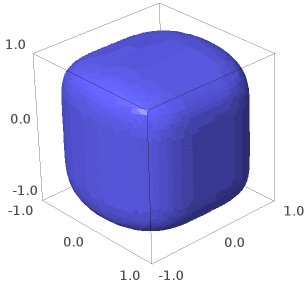
\includegraphics[width=6cm,height=5.60cm]{img/cubo_suave.png}
\caption{Representación (de sage) de $x^2+y^4+z^6=1$. Parece un cubo de lado 1 con aristas suaves.}
\label{fig:cuboSuave}
\end{figure}

\end{problem}

\begin{problem}[2]
Prueba que no existe una métrica Riemanniana en un toro $T$ tal que $K$ sea distinta de 0 y no cambie de signo en todo $T$
\solution

\doneby{Pedro} \approvedby{Guille}

En el toro hay una métrica riemanniana, la del \fref{ej:Superficies-1}, con curvatura $K$ idénticamente nula, lo que demuestra que para todo campo de vectores con singularidades aisladas la suma de los índices es nula.

Esta afirmación es sencilla de comprobar basándonos en el Teorema de Gauss Bonnet, que dice que
\[\frac{1}{2π}\int_M Kσ = \sum_{p_i} I_{p_i}(x)\]

Para una métrica riemanniana tal que su curvatura $K$ no es idénticamente nula, la integral de la curvatura es, otra vez por el teorema de Gauss-Bonnet y debido a que la suma de los índices no depende de la métrica riemanniana, nula, de forma que necesariamente tiene que haber puntos en los que $K$ es positiva y otros en los que es negativa.

De hecho, la integral de $Kσ$ sobre el conjunto de puntos en los que la curvatura es positiva tiene que ser igual y de signo contrario a la integral de $Kσ$ sobre los puntos en los que la curvatura es negativa (de otro modo no podríamos obtener 0).

\end{problem}

\begin{problem}[3]
Sea $M^2$ una variedad orientable y compacta de dimensión dos. Prueba que las siguientes afirmaciones son equivalentes (Asume que si $\chi(M^2)=\chi(\overline{M}^2)$ entonces $M^2$ es homeomorfa a $\overline{M}^2$):
\begin{enumerate}
\item[a)] Existe un campo de vectores en $M^2$ que nunca se anula

\item[b)] $\chi(M^2)=0$

\item[c)] $M^2$ es homeomorfo a un toro.
\end{enumerate}
\solution

\doneby{Pedro}

Vamos a demostrar las implicaciones necesarias una a una:
\begin{itemize}
\item $a) \implies b)$

Si hay un campo de vectores que no se anula, la suma de los índices es nula y sabemos, por el toerema de Poincaré, que esa suma es igual a la característica de Euler-Poincaré de $M$ ($\chi (M)$)

\item $c) \implies a)$

Hay un teorema que afirma que \textbf{si dos superficies son compactas y homeomorfas, son también difeomorfas}. Usando esto podemos afirmar que como en un toro hay campos de vectores que no se anulan, también los hay en cualquier superficie homeomorfa a un toro.

\item $b) \implies c)$

Un toro $T_2$ tiene característica de Euler-Poincaré $\chi (M)=0$ ya que, como en la circunferencia hay campos sin ceros, en el producto cartesiano de dos circunferencias hay campos sin ceros.

La asunción que nos insta a hacer el enunciado nos garantiza que si las características de Euler-Poincaré coinciden, las variedades son homeomorfas

\end{itemize}

Creo que se lió el profesor con las implicaciones que puso en su solución. Añade además una demostración de que $c) \implies b)$ y es que si dos superficies son homeomorfas, tendrán la misma característica de Euler-Poincaré ya que esta no depende de la triangulación.



\end{problem}

\begin{problem}[4]
 Sea $M^2 \subset \real^3$ una superficie regular en $\real^3$. Supongamos que $M^2$ es compacta, orientada y no homeomorfa a una esfera. Demuestra que existen tres puntos en $M^2$ para los que la curvatura Gaussiana es positiva, negativa, y 0.
\solution

\doneby{Edu}

Suponiendo que $M^2$ quiere decir que $M$ tiene dimensión 2, al ser subvariedad compacta y regular, suponemos que podemos encontrar una inmersión compatible con la topología $F: M \hookrightarrow \real^3$ función diferenciable tal que $F$ sea inyectiva sobre su imagen y rango $\Dif F = 2$.

Suponemos por el ejercicio anterior que al no ser $M$ homeomorfa a la esfera, debe tener $\chi \neq 2$.

Ahora hay que hacer algo con campos para aplicar Gauss-Bonnet que no se me ocurre. Tiene que ver con que la integral sobre $M$ dé 0 y para ello la curvatura deba cambiar de signo (y por lo tanto pasar por 0).

\approvedby{Guille}

Aquí el problema que veo es que podemos encontrar variedades, como el hiperboloide cortado, con curvatura negativa en todo punto y que son compactos. Tiene que haber algo en el enunciado que quite estos monstruos y sirva la sugerencia de Edu.


\end{problem}

%%%%%%%%%%%%%%%%%%%%%%%%%%%%%%%%%%%%%%%%%%%%%%%%%%%%%%%%%%%%%%%%%%%%%%%%%%%%%%%%%%%%%%%%%%%%%%%%%%%%
%%%%%%%%%%%%%%%%%%%%%%%%%%%%%%%%%%%%%%%%%%%%%%%%%%%%%%%%%%%%%%%%%%%%%%%%%%%%%%%%%%%%%%%%%%%%%%%%%%%%
%%%%%%%%%%%%%%%%%%%%%%%%%%%%%%%%%%%%%%%%%%%%%%%%%%%%%%%%%%%%%%%%%%%%%%%%%%%%%%%%%%%%%%%%%%%%%%%%%%%%
%%%%%%%%%%%%%%%%%%%%%%%%%%%%%%%%%%%%%%%%%%%%%%%%%%%%%%%%%%%%%%%%%%%%%%%%%%%%%%%%%%%%%%%%%%%%%%%%%%%%
%%%%%%%%%%%%%%%%%%%%%%%%%%%%%%%%%%%%%%%%%%%%%%%%%%%%%%%%%%%%%%%%%%%%%%%%%%%%%%%%%%%%%%%%%%%%%%%%%%%%
\newpage
\section{fasc-4-ejemplos}

\subsection{Variedades}
\begin{problem}[2]
Estudiar, siguiendo el modelo de $S^2$ la estructura de variedad diferenciable, con dos cartas, en $S^n$

\solution
\doneby{Pedro}

Comenzamos considerando una esfera de radio 1 en $\real^n$ que tendrá la ecuación:
\[\sum_{i=1}^n x_i^2=1\]
y describiendo explícitamente el atlas de dos cartas dado por la proyección estereográfica.

Siguiendo el ejemplo de la hoja, consideramos la proyección tomando el polo norte $(1,0...0)$ y el plano $x_1=-1$. Posteriormente construiremos la segunda carta tomando el polo sur $(-1,0...0)$ y el plano $x_1=1$. Vamos a ello.

\textbf{Primera carta}

\begin{itemize}
\item Supongamos un punto $p$ cualquiera del plano $x_1=-1$:
\[p=(-1,x_2,...x_n)\]

Si construimos la recta que lo une con el polo norte y la intersecamos con la esfera $S^n$ obtenemos el punto intersección $q$.
\[q = \left(1-2t, x_2\cdot t,...,x_n\cdot t\right)\]
Si el punto es la intersección con la esfera, su módulo deberá ser 1. Utilizamos este dato para calcular $t$.

\[1+4t^2-4t+t^2\left(\sum_{i=2}^nx_i^2\right)=1 \implies 4t^2-4t+t^2\left(\sum_{i=2}^nx_i^2\right) = 0 \implies t=\frac{4}{\sum_{i=2}^nx_i^2+4}\]

Por tanto el punto de intersección es:
\[q=\left(1-\frac{8}{\sum_{i=2}^nx_i^2+4}, \frac{4x_2}{\sum_{i=2}^nx_i^2+4},...,\frac{4x_n}{\sum_{i=2}^nx_i^2+4} \right)\]

\item Al revés. Empezamos ahora con un punto
\[x\in S^n\tq x=(α_1...α_n) \text{ con } \sum_{i=1}^n α_i^2 = 1\]

Construimos ahora el vector que une este punto con el polo norte y lo intersecamos con el plano $x_1=-1$

La recta unión con el polo norte queda de la forma:
\[\left(1+t(α_1+1),α_2t,...,α_nt \right)\]
y forzamos la intersección de esta recta con el plano para conocer el punto
\[1+t(α_1+1)=-1 \implies t = \frac{-2}{α_1+1}\]
con lo que el punto sería:
\[\left( -1, \frac{-2α_2}{α_1-1}, ..., \frac{-2α_n}{α_1-1}\right)=\left( -1, \frac{2α_2}{1-α_1}, ..., \frac{2α_n}{1-α_1}\right)\footnote{En el ejmplo de la hoja creo que escriben $α_1$ en función de las otras coordenadas, pero no veo necesaria esta complicación}\]
\end{itemize}

\textbf{Segunda carta}
\begin{itemize}
\item Supongamos un punto $p$ cualquiera del plano $x_1=1$:
\[p=(1,x_2,...x_n)\]

Si construimos la recta que lo une con el polo sur y la intersecamos con la esfera $S^n$ obtenemos el punto intersección $q$.
\[q = \left(-1+2t, x_2\cdot t,...,x_n\cdot t\right)\]
Si el punto es la intersección con la esfera, su módulo deberá ser 1. Utilizamos este dato para calcular $t$.

\[1+4t^2-4t+t^2\left(\sum_{i=2}^nx_i^2\right)=1 \implies 4t^2-4t+t^2\left(\sum_{i=2}^nx_i^2\right) = 0 \implies t=\frac{4}{\sum_{i=2}^nx_i^2+4}\]

Por tanto el punto de intersección es:
\[q=\left(-1+\frac{8}{\sum_{i=2}^nx_i^2+4}, \frac{4x_2}{\sum_{i=2}^nx_i^2+4},...,\frac{4x_n}{\sum_{i=2}^nx_i^2+4} \right)\]

\item Al revés. Empezamos ahora con un punto
\[x\in S^n\tq x=(α_1...α_n) \text{ con } \sum_{i=1}^n α_i^2 = 1\]

Construimos ahora el vector que une este punto con el polo sur y lo intersecamos con el plano $x_1=1$

La recta unión con el polo sur queda de la forma:
\[\left(-1+t(α_1+1),α_2t,...,α_nt \right)\]
y forzamos la intersección de esta recta con el plano para conocer el punto
\[-1+t(α_1+1)=1 \implies t = \frac{2}{α_1+1}\]
con lo que el punto sería:
\[\left( 1, \frac{-2α_2}{α_1+1}, ..., \frac{-2α_n}{α_1+1}\right))\]
\end{itemize}

Estudiamos ahora un punto cualquiera del plano $(-1,...x_n)$. Si lo mandamos en la esfera por la primera proyección que hemos calculado, llegamos al punto
\[\left(1-\frac{8}{\sum_{i=2}^nx_i^2+4}, \frac{4x_2}{\sum_{i=2}^nx_i^2+4},...,\frac{4x_n}{\sum_{i=2}^nx_i^2+4} \right)\]

Ahora calculamos la imagen directa de este punto por la segunda proyección estereográfica, con lo que llegamos a:
\[\left( 1, \frac{-2\frac{4x_2}{\sum_{i=2}^nx_i^2+4}}{2-\frac{8}{\sum_{i=2}^nx_i^2+4}}, ..., \frac{-2\frac{4x_n}{\sum_{i=2}^nx_i^2+4}}{2-\frac{8}{\sum_{i=2}^nx_i^2+4}}\right)=\left( 1, \frac{-4x_2}{\sum_{i=2}^nx_i^2},...,\frac{-4x_n}{\sum_{i=2}^nx_i^2}\right)\]

y podemos ver que se trata de un difeomorfismo sobre su imagen

\textcolor{blue}{En algún punto he metido la gamba con los signos porque debería salirme todo positivo. Pero ya he currado mucho con este ejercicio. Una paja y a seguir.}

\end{problem}



\begin{problem}[3]
Parametrizamos los puntos del hemisferio norte de la esfera $x_2 > 0$,
excluyendo el ecuador ($x_2 = 0$), en la forma $(θ, τ, + \sqrt{1 − θ^2 − τ^2})$ con
$θ^2 + τ^2 < 1$. Esto convierte al hemisferio norte en una carta coordenada, y podemos cubrir la esfera con seis cartas de este tipo tomando
como ecuador cada una de las intersecciones de la esfera con los planos
coordenados. Comprobar que, efectivamente, se trata de un atlas.

Demostrar que los dos atlas son equivalentes, viendo que los cambios
de carta de una carta de uno de ellos a una carta del otro inducen difeomorfismos.

\solution

\doneby{Guille}

Las seis cartas van a estar dadas por las siguientes parametrizaciones, todas con el mismo espacio de partida: \[ (θ, τ, \pm \sqrt{1 − θ^2 − τ^2}); \quad (τ, \pm \sqrt{1 − θ^2 − τ^2}, θ);\quad (\pm \sqrt{1 − θ^2 − τ^2}, θ, τ) \]

En el fondo simplemente estamos haciendo las permutaciones de las coordenadas. La intersección de dos cartas, si no es vacía, será dos cuadrantes de la esfera. Como todo son permutaciones, vamos a estudiar por ejemplo la intersección de las cartas $f_1 = (θ, τ, \sqrt{1 − θ^2 − τ^2})$ y $f_2 = (τ, \sqrt{1 − θ^2 − τ^2}, θ)$. Entonces $\inv{f_2}(x,y,z) = (x,z)$, así que $f_1 ○ \inv{f_2} = (θ, \sqrt{1 − θ^2 − τ^2})$, que es un difeomorfismo ya que su jacobiano es \[ \begin{pmatrix} 1 & \frac{2θ}{\sqrt{1 − θ^2 − τ^2}} \\ 0 & \frac{2τ}{\sqrt{1 − θ^2 − τ^2}} \end{pmatrix} \] distinto de cero en todo punto salvo en $τ = 0$. La cuestión es que ese punto no nos importa porque tal y como hemos construido las cartas, los puntos de la forma $(x, 0, z)$ no están en la imagen de $f_2$.

Con el resto de cartas saldría igual sólo que cambiando las cosas de orden, así que no me voy a preocupar mucho de sacarlo.

\end{problem}

\begin{problem}[4]
Demostrar que no existe ninguna variedad diferenciable compacta que se pueda recubrir con una única carta coordenada
\solution

\doneby{Pedro}

Si una variedad se puede recubrir por una única carta será homeomorfa a un abierto de $\real^n$ y, consecuentemente, nunca podrá ser compacta.

Esta respuestá está basada en la proposición 1.28 del documento: \href{http://ocw.um.es/ciencias/geometria-y-topologia/material-de-clase-1/01-variedadesdiferenciablessubvariedades-v100901.pdf}{Variedades Diferenciales y Subvariedades.pdf}
\end{problem}

\begin{problem}[5]
Demostrar que toda variedad 1-dimensional compacta y conexa es difeomorfa a la circunferencia $S^2$
\solution

\doneby{Pedro}

Para empezar es obvio que en caso de haber un difeomorfismo entre una variedad y la circunferencia, la variedad ha de ser compacta y conexa, pues así lo es la circunferencia.

Para resolver este ejercicio me baso en la proposición VI.1.6 de \href{https://books.google.es/books?id=CAOjRFAMJFUC&pg=PA131&lpg=PA131&dq=variedad+1-dimensional&source=bl&ots=MLkMP7HMyo&sig=aLLSSaYknqPZhPsn-5jJM2MwPAc&hl=es&sa=X&ei=DeMeVZSOEczZPdLkgfgJ&ved=0CCcQ6AEwAQ#v=onepage&q&f=false}{documento.pdf}. Básicamente la copio como un bellaco pero ahí dejo el link para el que quiera profundizar.

\textcolor{blue}{Justo en la versión que se puede consultar gratis en Google han quitado las dos páginas clave en que salía esto. El lunes pillo el libro en ciencias y lo completo}

\end{problem}

\begin{problem}[6]
Demostrar, como consecuencia del teorema de invarianza del dominio, que si $n \neq m$, no pueden ser homeomorfos $\real^n$ y $\real^m$. Tampoco es posible que sean homeomorfos un abierto de $\real^n$ con uno de $\real^m$
\solution

\doneby{Pedro}

En el fascículo 2 que podemos encontrar en moodle aparece la demostración de este hecho, que repetimos a continuación.

Supongamos abiertos $U \subset \real^n$ y $V\subset \real^m$ y la función $\appl{F}{U}{V}$ un difeomorfismo, es decir, una aplicación biyectiva, infinitamente diferenciable y con inversa infinitamente diferenciable.

\begin{enumerate}
\item Consideramos la función $G$ que es la función inversa de $F$, de forma que $G \circ F = 1_U$ y $F \circ G = 1_V$ siendo $1_X$ la identidad dentro del conjunto $X$.

\item Aplicando la regla de la cadena obtenemos:
\[G_{*,F(p)}\circ F_{*,p} = (1_U)_{*,p} \text{ y }  F_{*,p} \circ G_{*,F(p)} = (1_V)_{*,F(p)}\]

\item Pero, puesto que la matriz de la diferencial es la matriz jacobiana sabemos que
\[(1_U)_{*,p} = 1_{\tgs_p} \text{ y } (1_V)_{*,F(p)} = 1_{\tgs_{F(p)}}\]

\item Puesto que las aplicaciones $F_{*,p}$ y $G_{*,F(p)}$ son inversas la una de la otra los espacios $\tgs_p$ y $ 1_{\tgs_{F(p)}}$ son necesariamente isomorfos y por tanto $n$ y $m$ son iguales
\end{enumerate}

De hecho es imposible un \textbf{homomorfismo} entre abiertos de $\real^n$ y $\real^m$ pero esto se trata de un resultado topológico cuya demostración no entraría en el temario de este curso.

No obstante podemos encontrar esta última demostración en el siguiente \href{http://www.cmat.edu.uy/~rpotrie/documentos/pdfs/invarianciadimension.pdf}{documentopdf}
\end{problem}

\begin{problem}[7]
Demostrar que, si $\appl{f}{M}{N}$ es una función continua y localmente inyectiva de variedades topologícas de dimensión $n$, entonces la imagen de todo abierto $U \subset M$ es un abierto de $N$. En particular, $f(M)\subset N$ debe ser un abierto, que puede ser toda la variedad $N$
\solution

\doneby{Pedro}

Esto es un resultado de Topología que no voy a rehacer ya que no le veo mucha relación con lo que estamos estudiando en esta asignatura.

Por comentar algo relacionado con lo que estamos viendo, he viso en Wikipedia, y cito textualmente: ``El teorema de la invariancia del dominio establece que una función continua y localmente inyectiva entre dos variedades topológicas n-dimensionales debe ser abierta.''
\end{problem}

\begin{problem}[8]
Sea $S$ el conjunto de sucesiones $\appl{σ}{\nat}{\real}$ de números reales.

Definimos una topología en $S$ exigiendo que todas las funciones naturales de proyección
\[\appl{μ_{i_1,i_2,...,i_n}}{S}{\real^n}\]
sean continuas.\footnote{Estas funciones básicamente llevan la sucesión a un vector de $\real^n$ formado por $n$ elementos de la sucesión.}

Definimos una función $\appl{F}{S}{S}$ mediante
\[F(x_0,x_1,...,x_n,...)=(x_1,x_2,...,x_n,...)\]
Demostrar que la función $F$ es continua e inyectia, pero su imagen no es un abierto de $S$

\solution


\end{problem}

\begin{problem}[9]
Sea $U$ una bola unidad abierta en $\real^n$. Comprobar que la aplicación
\[f(\vx)=\frac{\vx}{\sqrt{1-\norm{\vx}^2}}\]
es un difeomorfismo de $U$ en todo $\real^n$
\solution

\yoP

Para comprobar que $f$ es un difeomorfismo debemos ver que es diferenciable, biyectiva y con inversa diferenciable. Vamos a ello.

La función, descompuesta en coordenadas, queda de la forma:
\[f(\vx)=\left(\frac{x_1}{\sqrt{1-\norm{\vx}}}, \frac{x_2}{\sqrt{1-\norm{\vx}}}, ..., \frac{x_n}{\sqrt{1-\norm{\vx}}}\right)\]

Vamos a derivarla:
\[\frac{\partial f}{\partial x_i}=\left(\frac{x_1x_i}{(\sqrt{1-\norm{\vx}})^3},\frac{x_2x_i}{(\sqrt{1-\norm{\vx}})^3},..\frac{1}{\sqrt{1-\norm{\vx}}}+\frac{x_i^2}{(\sqrt{1-\norm{\vx}})^3}.,\frac{x_nx_i}{(\sqrt{1-\norm{\vx}})^3}\right)\]

Podemos observar que la derivada existe (y por tanto la función es diferenciable) en todo punto con norma distinta de 1. Puesto que nos estamos restringiendo a $U$ que es la bola unidad \textbf{abierta} no hay problema con esto.

Podemos ver de manera sencilla que la función es inyectiva pues la derivada nunca se anula y podemos ver que es sobreyectiva por construcción. Para cualquier punto de $\real^n$ que tomemos podemos escribirlo como $f(\vx)$\footnote{Esto queda claro al calcular la función inversa, cosa que haremos a continuación}.

Por último nos queda estudiar la inversa.

\[f(\vx)=\vy \implies (y_1,....y_n)=\left(\frac{x_1}{\sqrt{1-\norm{\vx}}}, \frac{x_2}{\sqrt{1-\norm{\vx}}}, ..., \frac{x_n}{\sqrt{1-\norm{\vx}}}\right)\]

A ojo de buen cubero podemos ver que la función inversa sería
\[f^{-1}(\vy)=\frac{\vy}{\sqrt{1+\norm{\vy}}}\]
cosa que podemos comprobar fácilmente.

Resulta también trivial la observación de que esta función inversa también es diferenciable, por lo que queda claro que $f$ es un difeomorfismo.
\end{problem}

\begin{problem}[10]
Sea llama \textbf{Inversión en la esfera unidad de $\real^{n+1}$} a la aplicación $\appl{f}{\real^{n+1}\setminus \{0\}}{\real^{n+1}\setminus \{0\}}$ siendo
\[f(\vx)=\frac{1}{\norm{\vx}^2} \cdot \vx\]

Comprobar que se trata de un difeomorfismo que deja la esfera invariante, y establece un difeomorfismo entre el interior y el exterior de ella. En variable compleja esta inversión, en la circunferencia unidad del plano complejo, se escribe:
\[f(z)=\frac{z}{|z|^2}=\frac{z}{z\cdot \bar{z}} = \frac{1}{\bar{z}}\]

\solution
\doneby{Pedro}

Esta función es evidentemente continua salvo en el origen, que no se incluye. Podemos escribirla como: (tomando una única coordenada):
\[f_i(\vx)=y_i=\frac{x_i}{\norm{\vx}^2}\]

Puesto que $\norm{\vy}=1/\norm{\vx}$ tenemos que:
\[y_i = x_i \cdot \norm{\vy}^2 \implies x_i = \frac{y_i}{\norm{\vy}^2}\]

y vemos que se trata también de una función continua.

Tanto la función $f$ como su inversa (para la que hemos encontrado una fórmula) son continuas y, viendo que ambas están definidas en todo $\real^{n+1}\setminus \{0\}$ podemos concluir que ambas son biyectivas (si una no fuese inyectiva no podríamos haber encontrado la otra y si no fuese sobreyectiva la inversa no estaría definida en todo el dominio).

Para comprobar la diferenciabilidad podemos derivar y ver que la derivada no da problemas fuera del origen.

Por último, puesto que la esfera está formada por todos los puntos con módulo 1, está claro que este difeomorfismo manda la esfera en sí misma.

\end{problem}

\begin{problem}[11]
Demostrar que si definimos variedades diferenciables con cartas coordenadas que valoran en bolas abiertas de $\real^n$, o con cartas que valoran en todo $\real^n$, se obtienen las mismas variedades que con la definición estándar que hemos usado.

\solution
\doneby{Pedro}

Recordemos la definición de \nlref{def:VariedadDiferenciable}. Lo que nos pide comprobar el problema es que estas propiedades se cumplen también con dos formas distintas de definir las cartas.

Con los resultados vistos en topología, podemos ver que el primer cambio es trivial. Si en lugar de considerar todos los abiertos posibles considero solo bolas abiertas no cambia nada, pues todas las bolas son abiertas y todo abierto puede escribirse como unión de bolas abiertas.

En el segundo caso tendríamos que tomar $U_i=X \ \forall i$ por lo que la función $f_i$ deberá extenderse a todo $X$ siendo $f_i(X \setminus U_i)=0$. No quiero pararme a rayarme mucho con esto, pero se parece a lo que hacemos con las particiones de la unidad al extender formas en $U_i$ a todo $X$.

\end{problem}

\begin{problem}[14]
Considerar el conjunto de puntos $M \subset \real^3$ tales que su distancia (mínima) a la circunferencia, en el plano $z=0$, de centro el origen y radio $a$, sea exactamente $b$.

Demostrar que si $b< a$, podemos definir una estructura de variedad diferenciable en $M$, que es, de hecho, difeomorfa a $S^1 \times S^1$. ¿Qué ocurre si $b \geq a$?

\solution

\doneby{Pedro}

Si $b<a$ podemos ver que lo que estamos definiendo es como una rosquilla, es decir, tenemos el toro que ya sabemos que es homeomorfo a $S^1 \times S^1$. En concreto, puesto que es una variedad diferenciable tenemos un difeomorfismo.

Si $b<a$ lo que estamos definiendo es una estructura similar a una esfera aplastada y, por tanto, será difeomorfa a $S^1$

\end{problem}

\subsection{Campos}
\begin{problem}[1]
(\textbf{Grupos uniparamétricos de automorfismos}) En cada uno de los siguientes ejemplos se da una familia uniparamétrica de automorfismos de $\real^n$ y se pide que se compruebe que es un grupo y determine el campo asociado (\textbf{generador infinitesimal del grupo}). En todos los casos el grupo es un grupo de transformaciones lineales y el campo es un campo lineal (coeficientes de grado a lo más uno)

\ppart Grupo de traslaciones
\[τ_1(x_1,...,x_n)=(x_1+t,x_2,...,x_n)\]

\ppart Grupo de homotecias
\[τ_t(x_1,...,x_n)=(e^tx_1, e^tx_2,...,e^tx_n)\]

\ppart Sea $A$ una matriz $n\times n$. Definimos un grupo uniparamétrico de automorfismos, asociado a la matriz $A$, mediante
\[τ_t(X)=e^{tA}X\]
¿Es el primer ejemplo un caso particular de este?

\ppart
Supongamos ahora $n=2$, y sea
\[ \left( \begin{array}{cc}

\cos(t) & -\sin(t) \\
\sin(t) & \cos(t)

\end{array} \right)\]
la matriz de una rotación de ángulo variable $t$ en el plano. Definimos un grupo uniparamétrico de automorfismos
\[τ_t(x_1,x_2)=A(t)\cdot {x_1 \choose x_2}\]

¿Es este ejemplo un caso particular del c)?

\solution
\yoP

Para demostrar que cada uno de estos conjuntos es un grupo debemos identificar la operación que define el grupo, demostrar que es asociativa y encontrar el elemento neutro o identidad y el inverso.

\spart
La operación suma se define de la siguiente forma:
\[(τ_a+τ_b)(x_1,...,x_n)=(x_1+a+b,x_2,...,x_n)\]

Es evidente que la operación es asociativa, el elemento neutro es $τ_0$ y el inverso de $τ_t$ es $τ_{-t}$

Queda claro que es un grupo.

Vamos a encontrar el campo asociado. La teoría de lo que vamos a hacer a continuación viene en las páginas 73-74 de \href{http://matematicas.unex.es/~ricarfr/EcDiferenciales/LibroEDLat.pdf}{documento.pdf}

Básicamente nos da un teorema y su demostración. El teorema dice:

Sea $X$ un grupo uniparamétrico local de clase $k$. Para cada $f\in C^{\infty}(U)$ y $p \in U$ definimos
\[(Df)(p)=\lim_{t \to 0}\frac{f[X(t,p)]-f(p)}{t}\]
entonces $D \in D_k(U)$ y lo llamaremos generador infinitesimal de X.

El ejemplo concreto que vamos a hacer (o uno muy similar) así como los siguientes vienen resueltos al final de la página 16 de \href{http://matematicas.unex.es/~ricarfr/EcDiferenciales/LibroEDLat.pdf}{documento.pdf}

Así para este ejemplo tendríamos la aplicación flujo $\appl{\phi}{\real^{n+1}}{\real^n}$ siendo $\phi(x_1,...,x_n,t)=(x_1+t,x_2,...,x_n)$.

\[X = \left(\frac{\partial \phi}{\partial t}\right)_{t=0} \frac{\partial}{\partial x_i}=\frac{\partial}{\partial x}\]


\textbf{Del último documento mencionado cabe destacar:}

\begin{defn}[Generador\IS infinitesimal]
Sea $\{σ_t\}$ un grupo monoparamétrico de transformaciones de U. Llamamos \textbf{generador infinitesimal} de $\{σ_t\}$ al campo vectorial que asigna al punto $p$, el vector tangente a la curva $(-ε,ε)\to U$, $t \to σ_t(p)$

Consideremos $\appl{\phi}{\real \times U}{U}$ la aplicación flujo del grupo $\phi(t,p)=σ_t(p)$. entonces el generador infinitesimal puede considerarse
\[X = \sum_{i=1}^n \left( \frac{\partial \phi_i}{\partial t}\right)_{t=0}\frac{\partial}{\partial x_i}\]
\end{defn}

\end{problem}

\begin{problem}[2]
Sea $D$ el campo en $\real^2$ definido como
\[D=x \frac{\partial}{\partial x}+y \frac{\partial}{\partial y }\]

El campo está definido en todo el plano pero

\ppart Una integral primera definida en todo el plano es necesariamente constante

\ppart Para cada punto, diferente al origen hay un entorno en el que hay una integral primera. Determinar todas esas integrales primeras no globales y los abiertos máximos en que están definidas.
\solution


\yoP

\spart
Vamos a tratar de resolver y buscar la integral primera: funciones $H$ tales que $D(H) = 0$. Para ello, resolvemos el par de ecuaciones
\begin{align*}
\frac{\partial H}{\partial x} &= \frac{1}{x} \implies H(x,y)=\log(x)+f(y)\\
\frac{\partial H}{\partial y} &= \frac{1}{y} \implies H(x,y)=\log(y)+g(x)
\end{align*}

De donde concluimos que $H(x,y)=\log(x)+\log(y)$. El problema de esta integral primera es que no está definida en todo el plano.

Tenemos que buscar otra forma de encontrar integrales primeras definidas en todo el plano. Para ello resolvemos el sistema
\begin{align*}
\frac{\partial H}{\partial x} &= -y \implies H(x,y)=-xy+f(y)\\
\frac{\partial H}{\partial y} &= x \implies H(x,y)=yx+g(x)
\end{align*}

No hay elección posible de $f$ y $g$ que resuelva ese sistema. Sin embargo, el campo es no nulo en todo punto salvo en $(0,0)$, y tienen que existir integrales primeras en entornos de esos puntos. Así, sólo nos queda una opción, que $\dpa{H}{x} = \dpa{H}{y} = 0$, luego $H(x,y)$ tiene que ser constante.

Otro punto de vista es el siguiente: si resolvemos el sistema de EDOs asociado \begin{align*}
x'(t) &= x(t) \\
y'(t) &= y(t)
\end{align*} nos queda que las curvas solución son de la forma $γ(t) = (c_1e^t, c_2e^t)$. Cuando $t = 0$, $γ(0) = (c_1, c_2)$ luego está claro que las constantes son las coordenadas del punto inicial de la curva $(x_0, y_0) = (c_1, c_2)$.

Haciendo el corte de γ con el plano $x = 1$, tenemos \[ 1 = x_0e^t \implies t = - \log x_0 \], y sustituyendo en la ecuación de la segunda coordenada queda $y = \frac{y_0}{x_0}$, que efectivamente son curvas constantes.

\spart Retomamos el primer cálculo de integral primera que hicimos: $H(x,y)=\log(x)+\log(y)$

Estas integrales primeras están definidas en todo punto salvo en los ejes de coordenadas.

\end{problem}

\begin{problem}[3]
Estudiar el campo en el plano definido como
\[D=(y+x(1-x^2-y^2))\frac{\partial}{\partial x} + (-x+y(1-x^2-y^2))\frac{\partial}{\partial y}\]
usando, si te parece conveniente, un cambio a coordenadas polares.
\solution
\yoP

Vamos a ver las curvas solución o curvas integrales del campo. Básicamente esto consiste en buscar una función tal que en todo punto su vector tangente sea el dado por D. Es decir, que su derivada coincida con el campo.

Buscamos $\appl{α}{I}{\real^2}$ siendo $α(t)=(x(t),y(t))$, tal que
\begin{align*}
\frac{dx}{dt} &= y+x(1-x^2-y^2) \\
\frac{dy}{dt} &= -x+y(1-x^2-y^2)
\end{align*}

Dado que esto parece un tanto inmanejable vamos a atender al consejo dado y pasamos todo a coordenadas polares. Así el campo quedaría:
\[D=(r(\sin(\theta)+\cos(\theta)(1-r^2)))\left(\cos(\theta)\frac{\partial}{\partial r} - r\sin(\theta)\frac{\partial}{\partial \theta} \right)+\]
\[+(r(-\cos(\theta)+\sin(\theta)(1-r^2)))\left(\sin(\theta)\frac{\partial}{\partial r} + r\cos(\theta)\frac{\partial}{\partial \theta} \right)\]
operando un poco podemos dejarlo más bonito como:
\[D= r(1-r^2)\frac{\partial}{\partial r}+(-r^2)\frac{\partial}{\partial \theta}\]

En estas condiciones podemos considerar $\alpha(t)=(r(t),\theta(t))$ y al buscar la curva integral nos quedaría el sistema de ecuaciones:
\begin{align*}
\frac{dr}{dt} &= r(1-r^2) \implies dt = \frac{dr}{r-r^3} \implies t=\log(r)-\frac{1}{2}\log(1-r^2) \\
\frac{d\theta}{dt} &= r^2 \implies d\theta=\frac{r^2dr}{r-r^2} \implies \theta = \frac{1}{2}\log(1-r^2)
\end{align*}

Si despejamos $r$ de la primera ecuación obtenemos:
\[ \log(1-r^2) = 2 (\log r - t) \]
\[ 1 - r^2 = r^2 e^{-2t} \iff  1 = r^2 (1 + e^{-2t}) \]
\[ r^2 = \frac{1}{1 + e^{-2t}} \]
Luego
\[ \alpha(t) = \left( \sqrt{\frac{1}{1 + e^{-2t}}} - (\frac{1}{1 + e^{-2t}})^{3/2}, -\frac{1}{1 + e^{-2t}} \right) \]

\end{problem}

\begin{problem}[5]
Para cada uno de los campos $D_i$, definido en un abierto $U_i$ encontrar un sistema de coordenadas en el que el campo se endereza

\ppart
\[D_1 = x \frac{\partial}{\partial x}+2y\frac{\partial}{\partial y} \text{ siendo } U_i=\{(x,y) \tq x > 0\}\]

\ppart
\[D_2 = \frac{\partial}{\partial x}+\sin(x)\frac{\partial}{\partial y} \text{ siendo } U_2 = \real^2\]

\ppart
\[D_3 = x\frac{\partial}{\partial x}+(1-x^2)\frac{\partial}{\partial y} \text{ siendo } U_3 = \{(x,y) \tq -1 < x < 1\}\]

\solution

\spart
Para enderezar el campo calculamos su integral primera:
\[0 = D(H) = x\frac{\partial H}{\partial x}+2y\frac{\partial H}{\partial y}\]
Para resolver esta ecuación debemos resolver el sistema:
\begin{align*}
\frac{\partial H}{\partial x} &= -2y\\
\frac{\partial H}{\partial y} &= x
\end{align*}

de donde obtenemos nada porque no sale. Cuando esto no conduce a nada directamente, el remedio es calcular las curvas solución. Resolvemos
\begin{align*}
\od{x}{t} &= x \\
\od{y}{t} &= 2y
\end{align*} y nos da que
\begin{align*}
x(t) &= e^t x(0) \\
y(t) &= e^{2t} y(0)
\end{align*}

Ahora tenemos que cortar estas curvas solución con un plano. No puede ser el plano $x = 0$ porque no pasan por $x = 0$. Cortamos por un plano $y_0$ que no sé qué es, parece que es el punto donde estamos enderezando el campo. Resolvemos
\[ e^{2t} y(0) = y_0 \implies t = \frac{\log y_0 - \log y(0)}{2} \], que sustituyendo en $x(t)$ nos da \[ x = e^{\frac{\log y_0 - \log y(0)}{2}} x(0) = x \sqrt{\frac{y_0}{y(0)}} \] y entonces la función $H$ que buscamos es \[ H(x,y) =  x \sqrt{\frac{y_0}{y}} \]

Para enderezar el campo, hay que aplicar una fórmula de la que el profesor no se acuerda. A veces se ve pero en otros casos hay que hacer una integral de una función de $n$ variables integrando con respecto a una de ellas y en general es horroroso y no lo vamos a ver.

\spart

Para enderezar el campo calculamos su integral primera
\[0 = D(H) = \frac{\partial H}{\partial x}+\sin(x)\frac{\partial H}{\partial y}\]
Para resolver esta ecuación debemos resolver el sistema:
\begin{align*}
\frac{\partial H}{\partial x} &= -\sin(x)\\
\frac{\partial H}{\partial y} &= 1
\end{align*}

de donde obtenemos $H(x,y)=\cos(x)+y$

Ahora debemos buscar una función $G$ tal que $D(G)=1$ para ello basta con tomar $G(x,y)=x$

¿Determinan las funciones $H$ y $G$ un sistema de coordenadas locales? Para ello debemos estudiar el rango de su matriz jacobiana:
\[\left( \begin{array}{cc}
-\sin(x) & 1  \\
1 & 0  \end{array} \right)\]

y vemos que el determinante es siempre 1 por lo que tenemos un sistema de coordenadas locales en el entorno de cualquier punto del plano. Si conseguimos probar que el cambio de coordenadas es biyectivo, tendremos un sistema de coordenadas definido en todo el plano $\real^2$.

Tenemos pues el cambio de coordenadas:
\begin{align*}
x_1 &= \cos(x)+y\\
y_1 &= x
\end{align*}

que es claramente invertible siendo:
\begin{align*}
x = y_1\\
y = x_1 - \cos(y_1)
\end{align*}

Entonces, el campo $D$ se endereza en un sistema de coordenadas definido en todo el plano.

\spart
\yoP

Buscamos nuevamente una función $H$ que sea integral primera del campo. En este caso no es posible calcularla directamente, de modo que tendremos que hacer algo parecido a lo que hacíamos en el apartado \textbf{a)}.

Calculamos directamente la curva solución del campo:
\begin{align*}
\dot{x}&=x \implies x(t)=e^tx(0)\\
\dot{y}&=(1-x^2) \implies y(t)=\int 1-e^{2t}x(0)^2 dt \implies y(t)=t-\frac{e^{2t}x(0)^2}{2}+y(0)+\frac{x(0)^2}{2}
\end{align*}

Tomamos un punto en el que el campo no se anule como puede ser el punto $(1,0)$. Ahora debemos tomar una hipersuperficie que no contenga al vector $D_p$, que será el plano $x=1$. Veamos en qué punto la curva solución corta a esta hipersuperficie:

\[e^t x(0)= 1 \implies t = \log\left(\frac{1}{x(0)}\right)\]
lo que nos da un valor de la segunda coordenada del punto:
\[y(t)=\log\left(\frac{1}{x(0)}\right)-\frac{1}{2}+y(0)+\frac{x(0)^2}{2}\]

Concluimos que la integral primera del campo sería:
\[H(x,y)=\log\left(\frac{1}{x}\right)-\frac{1}{2}+y+\frac{x^2}{2}\]

Para cerciorarnos de que todo está bien podemos comprobar de forma sencilla que $D(H)=0$.

Para terminar de enderezar el campo deberíamos encontrar una función $G$ tal que $D(G)=1$. Para ello basta con tomar $G(x,y)=\log(x)$. Así, nos queda que el cambio de variables que permite enderezar el campo es:
\begin{align*}
x_1 &= \log\left(\frac{1}{x}\right)-\frac{1}{2}+y+\frac{x^2}{2} \\
y_1 &= \log(x)
\end{align*}

Para comprobar en qué puntos este cambio de variables es válido estudiamos el rango de su matriz Jacobiana:

\[\left( \begin{array}{cc}
x-\frac{1}{x} & \frac{1}{x}  \\
1 & 0  \end{array} \right)\]

Pudiendo ver fácilmente que el rango es 2 salvo en $x=0$ donde se nos hace infinito y no estamos muy seguros de que ocurre.

A la hora de estudiar si el cambio de coordenadas es global posiblemente nos encontremos con que lo es salvo en los puntos con $x=0$. No obstante esta parte se deja como ejercicio para el lector.
\end{problem}

\begin{problem}[6]
Calcula el laplaciano
\[\frac{\partial^2}{\partial x^2}+\frac{\partial^2}{\partial y^2}\]

en coordenadas polares

\solution
\yoP

Siendo $x=r\cos(α)$ e $y=r\sin(α)$ tenemos
\[2(-\sin(α)+\cos(α))\frac{\partial}{\partial r}\frac{\partial}{\partial α}+r(-\cos(α)-\sin(α))\frac{\partial^2}{\partial α^2}\]
\end{problem}

\begin{problem}[7]
Expresar en coordenadas cilíndricas $(x=ρ\cos(α), y=ρ\sin(α), z=z)$ el campo
\[D= 2 \frac{\partial}{\partial x}-\frac{\partial}{\partial y}+3\frac{\partial}{\partial z}\]

\solution
\yoP

Simplemente tendremos que aplicar en la ecuación del campo los cambios:
\begin{align*}
\frac{\partial}{\partial x} &= \cos(α)\frac{\partial}{\partial ρ}-ρ\sin(α)\frac{\partial}{\partial α} \\
\frac{\partial}{\partial y} &= \sin(α)\frac{\partial}{\partial ρ}+ρ\cos(α)\frac{\partial}{\partial α}
\end{align*}

Con lo que nos queda:
\[D=(2\cos(α)-\sin(α))\frac{\partial}{\partial ρ}-(2ρ\sin(α)+ρ\cos(α))\frac{\partial}{\partial α}+3\frac{\partial}{\partial z}\]

\end{problem}

\begin{problem}[8]
Consideramos los campos en $\real^3$

\begin{align*}
D_1 &=(2+y^2)e^z \frac{\partial}{\partial x}\\
D_2 &=2xy\frac{\partial}{\partial x}+(2+y^2)\frac{\partial}{\partial y}\\
D_3 &=2xy^2\frac{\partial}{\partial x} - y(2+y^2)\frac{\partial}{\partial y}+(2+y^2)\frac{\partial}{\partial z}
\end{align*}

\ppart Demostrar que estos tres campos generan, en cada punto de $\real^3$, el espacio tangente en el punto

\ppart
Calcular también 3 1-formas tales que, en cada punto de $\real^3$, determinen la base dual de la formada por los 3 campos dados.
\solution
\yoP

\spart
Para comprobar que los tres campos generan el espacio tangente basta con comprobar que los vectores que representan cada campo son linealmente independientes. Es decir, tenemos que ver que la siguiente matriz tiene rango máximo:
\[\left( \begin{array}{ccc}
(2+y^2)e^z & 0 & 0  \\
2xy & 2+y^2 & 0\\
2xy^2 & -y(2+y^2) & 2+y^2  \end{array} \right)\]

Podemos ver que el determinante de esta matriz es:
\[\left((2+y^2)e^z\right)\left(2+y^2 \right) \left(2+y^2 \right)\]
que podemos ver fácilmente que no se anula nunca, pues estamos siempre multiplicando términos no nulos.

\spart

Lo que nos están pidiendo son tres 1-formas $ω_i$ tales que $ω_i(D_j)=1$ si $i=j$ y $0$ en caso contrario. Lo que vamos a hacer es construir estas formas a mano, forzando que se cumplan estas propiedades:
\[ω_1 = \frac{1}{(2+y^2)e^z}+ady+bdz\]
con esto hemos asegurado $ω_1(D_1)=1$. Ahora calculamos $a$ y $b$ forzando $ω_1(D_2)=0$ y $ω_1(D_3)=0$.

Así nos queda
\[ω_1 = \frac{1}{(2+y^2)e^z}+- \frac{2xy}{(2+y^2)e^z(2+y^2)}dy+\left(-\frac{2xy^2}{(2+y^2)e^z})-\frac{2xy^2(2+y^2)}{(2+y^2)e^z(2+y^2)}\right)\frac{1}{2+y^2}dz\]

Ahora pasamos a calcular $ω_2$. Para forzar que al evaluarlo sobre el primer campo obtengamos un $0$ basta con hacer que no tenga componente dx. Y sabiendo que $ω_2(D_2)=1$ tenemos que
\[ω_2 = \frac{1}{2+y^2}dy+cdz\]
calculamos ahora $c$ forzando que $ω_2(D_3)=0$ con lo que nos queda:
\[ω_2 = \frac{1}{2+y^2}dy+\frac{y(2+y^2)}{(2+y^2)^2}dz\]

Por último y de forma trivial tenemos que
\[ω_3 = \frac{1}{2+y^2}dz\]

\textbf{Observación importante de Julián.}

Estas formas que hemos obtenido se corresponden con las filas de la inversa de la matriz de los campos. Este hecho que observamos y que podría parecer fortuito se produce siempre y tiene la siguiente explicación.

Si escribimos la matriz que tiene las formas $ω_i$ como filas y la multiplicamos por la izquierda por la matriz de los vectores de campo obtenemos en cada coordenada de la matriz solución:
\[a_{ij}=ω_i D_j\]
que coincide con la evaluación de la forma $ω_i$ en el campo $D_j$. Por la construcción de las $ω_i$, que son la base dual de la formada por los campos, obtenemos como resultado la matriz identidad.
\end{problem}

\begin{problem}[9] Sea $C = \gen{X,Y,Z}$ el espacio vectorial de dimensión 3 generado por los campos \[ X = z \dpa{}{y} - y\dpa{}{z} \quad Y = -z \dpa{}{x} + x \dpa{}{z} \quad Z = y\dpa{}{x} - x\dpa{}{y} \]

\ppart Demostrar que existe un isomorfismo $\appl{Φ}{C}{ℝ^3}$ tal que, para $D,D' ∈ C$, se tiene que \[ Φ([D,D']) = Φ(D) × Φ(D') \]

\ppart Demostrar que el flujo de un campo $D ∈ C$ está formado por rotaciones alrededor de un eje común. Encontrar la relación de ese eje con el vector $Φ(D)$.
\solution

\doneby{Guille}

\spart
El isomorfismo es $Φ(aX+bY+cZ) = (a,b,c)$, y hay que comprobar que el corchete de Lie es lo mismo que el producto vectorial.

\spart Tomamos por ejemplo el campo $X$. El campo es el mismo para todo $x$, luego sólo tenemos que considerar lo que ocurre en el plano $yz$. Y en ese plano, el campo es una rotación alrededor del origen. Es decir, que el flujo del campo $X$ son rotaciones a lo largo del vector $(1,0,0)$ que es casualmente $Φ(X)$.

Esto nos da la idea de que, para un campo $D$, el flujo va a ser una rotación alrededor del eje $Φ(D)$. Para demostrar esto, el profesor propone un argumento que consiste en transformar el eje de rotación en el $(1,0,0)$ de tal forma que se lleven flujos a flujos y demostrar que la rotación es alrededor de ese eje.

\end{problem}

\begin{problem}[10]
Sea $M \subset \real^3$ una subvariedad regular. Un \textbf{campo de vectores tangentes} en $M$ puede definirse como una función diferenciable $\appl{α}{M}{\real^n}$ tal que para cada punto $p \in M$ el vector $α(p)$ es tangente a $M$ en $p$.

Demostrar que las esferas de dimensión impar $S^{2n-1} \subset \real^{2n}$ admiten campos de vectores que no se anulan en ningún punto.

\solution

\doneby{Pedro}

La respuesta a este ejercicio ha sido obtenida de \href{http://divulgamat2.ehu.es/divulgamat15/index.php?option=com_docman&task=doc_download&gid=515}{aquí}.

Para demostrar la existencia del campo de vectores que no se anula en ningún punto, lo vamos a calcular.

Definimos el campo vectorial:
\[D(x_1,...,x_2n)=-x_2 \frac{\partial}{\partial x_1}+x_1\frac{\partial}{\partial x_2}+...-x_{2n}\frac{\partial}{\partial x_{2n-2}}+x_{2n-1}\frac{\partial}{\partial x_{2n}}\]
Evidentemente este campo no tiene 0 más que el origen. Para ver que es tangente a la esfera basta con ver que el vector normal de la esfera $(x_1,...,x_{2n})$ es perpendicular al campo.
\end{problem}

\begin{problem}[11]
En un toro de dimensión cualquiera $n$, que podemos ver como una subvariedad de $\real^n$ (¿CÓMO?), siempre existen $n$ campos tangentes que en cada punto determinan una base del espacio tangente. Por tener esta propiedad decimos que los toros son \textbf{variedades paralelizables}

\solution

\doneby{Pedro}

Un toro $n$ dimensional se define como el producto de $n$ circunferencias:
\[T^n = S^1 \times S^1 \times ... \times S^1\]

Es sencillo ver el toro como una subvariedad pues es el producto cartesiano de subvariedades.

Para ver los $n$ vectores tangentes basta con fijar una de las circunferencias que forman el producto cartesiano que da lugar al toro. En cada punto, tomamos como vector tangente el vector velocidad de la circunferencia al pasar por ese punto.

\end{problem}

\section{Ejercicios de Inmersiones}

Estos ejercicios son los de la última hoja que nos dió en clase impresa antes del parcial y que no está en moodle.

\begin{problem}[1]
Comprobar que la función $\appl{F}{\real}{\real^2}$ tal que
\[F(t)=\left( \frac{e^t+e^{-t}}{2}, \frac{e^t-e^{-t}}{2}\right)\]
es una inmersión inyectiva con imagen una de las ramas de la hipérbola $x^2-y^2=1$. De hecho, la inmersión es compatible con la topología, y la rama de la hipérbola es una subvariedad regular del plano.

Las componentes de $F$ son el seno y el coseno hiperbólico, que parametrizan la rama de la hipérbola de manera similar a como el seno y el coseno parametrizan la circunferencia unidad.

\solution

\doneby{Pedro}

Para ver que es una inmersión debemos ver que se trata de una función diferenciable con inversa inyectiva.

Es obvio\footnote{por ser composición de funciones diferenciables.} que la función es diferenciable luego sólo tenemos que comprobar la inyectividad de la diferencial y para ello basta con ver que la matriz Jacobiana no se anula.

\[ J=\left( \frac{e^t-e^{-t}}{2}, \frac{e^t+e^{-t}}{2}\right)\]
y, como podemos ver, este vector no se anula para ningún $t$ luego por el teorema de la función inversa, tenemos que F es un difeomorfismo entre $\real$ y F($\real$)


\doneby{Dejuan}

Para comprobar que la imagen está contenida en una de las ramas de la hipérbola, $F(t) = (cosh(t),senh(t)) = (x,y)$ y calculamos $x^2 - y^2 = cosh^2(t) - senh^2(t) = 1$ utilizando las propiedades de los hiperbólicos. Entonces $F(ℝ) \subset Ω = \{(x,y) \tq x^2 - y^2 = 1 \}$

Vamos a ver que es una imersión. Para ello, comprobamos que $DF$ es inyectiva. Para ello utilizamos la sugerencia de $F(t) = (cosh(t),senh(t))$ y razonamos: $DF = (senh(t),cosh(t))$ Sean $t_1,t_2∈ℝ$ tales que $F(t_1)=F(t_2)$. Entonces, $cosh(t_1) = cosh(t_2) \implies t_1 = t_2$. CQC. Otra posibilidad sería comprobar que $\ker DF = \{ 0 \}$


Comprobamos $F$ inyectiva (lo pide el enunciado) con el mismo argumento que antes: sean $t_1,t_2∈ℝ$ tales que $F(t_1)=F(t_2)$. Entonces, $cosh(t_1) = cosh(t_2) \implies t_1 = t_2$. CQC.


Ahora tenemos que ver que sea una subvariedad regular. Para ello tenemos 2 opciones, utilizar el \nref{thm:Inmersion} o el \nref{thm:Submersion}.

En este caso, como nada es compacto recurrimos al de submersión.

Definimos $H(x,y) = x^2 - y^2$ con $\appl{H}{ℝ^2}{ℝ^2}$ y comprobamos que $DH$ es sobreyectiva y esto es claro de ver, ya que $∀p∈ℝ$ tomamos $x = \sqrt{p}$ y tenemos $H(x,0) = p$.

Confiando en la sobreyectividad, podemos aplicar el teorema, que nos dice que $H^{-1}(q)$ es una subvariedad regular. Tomando $q=1$, tenemos que $H^{-1}(q) = Ω$ es una subvariedad del plano.


\end{problem}

\begin{problem}[2] Comprobar que la función $F(x,y)=(x,xy,y^2)$ es una inmersión excepto en el origen. ¿Es inyectiva? ¿Qué se puede decir de su imagen?

\solution

\doneby{Pedro}

La función es claramente diferenciable\footnote{por ser composición de polinomios.}. Vamos a mirar el Jacobiano para comprobar la inyectividad de la diferencial.

\[ J = \left( \begin{array}{cc}
1 & 0\\
y & x \\
0 & 2y \end{array} \right)\]

podemos ver que tenemos rango máximo en todo punto (salvo en el origen), por lo que es una inmersión (salvo en el origen).

La función $F$ es inyectiva puesto que dos puntos de $\real^3$ que coincidan tendrán preimágenes con igual $x$ (cosa que deducimos por la primera coordenada) y con igual $y$ (como deducimos por la segunda coordenada).


La imagen sería algo así como una hipérbola que tiene altura $y^2$, es decir, que va aumentando como una parábola según nos alejamos del origen.

\doneby{Dejuan}

De la imagen podemos decir que es una subvariedad regular. ¿BOOM?

Como antes, podríamos utilizar el teorema de inmersión o de submersión. Como nada es compacto, recurrimos al de submersión.

Necesitamos una $\appl{H}{\img F}{ℝ^3}$ con $DH$ sobreyectiva en algún punto.


Como tenemos varias variables, descomponemos: $\appl{F}{ℝ^2}{ℝ^3}$ en $\appl{F_i}{ℝ^2}{ℝ}$

\begin{align*}
\appl{F_1}{ℝ^2}{ℝ}\; F_1(x,y) = x \to & G_1(x,y,z) = x-z \to DG_1 = (1,0,-1)\\
\appl{F_2}{ℝ^2}{ℝ}\; F_2(x,y) = x \to & G_2(x,y,z) = xy-z \to DG_2 = (y,x,-1)\\
\appl{F_3}{ℝ^2}{ℝ}\; F_3(x,y) = x \to & G_3(x,y,z) = y^2-z \to DG_3 = (0,2y,-1)
\end{align*}

Ahora, suponiendo que $DG_i$ son sobreyectivas en $p=0$, podemos decir: $DG_i^{-1}(0)$ es una subvariedad regular por el teorema de Submersión, y que $DG_1^{-1}(0) × DG_2^{-1}(0) × DG_3^{-1}(0) $
es una subvariedad de $ℝ^3$ por ser producto de subvariedades.

Todo esto, suponiendo que las $DG_i$ son sobreyectivas, que lo vamos a comprobar ahora mismo. Para ello, utilizamos propiedades de álgebra conocidas como que una aplicación es sobreyectiva si la dimensión de su imagen es la dimensión del conjunto de llegada. En este caso, los 3 conjuntos de llegada son $ℝ$ y las 3 imágenes tienen dimensión 1 (en $p=0$ tenemos 1 vector en cada $DG_i$ cuya dimensión de la imagen es 1 (una recta) como en $ℝ$).

\end{problem}

\begin{problem}[3]
Si $M, N \subset \real^n$ son variedades regulares  y $M \subset N$, entonces $M$ es una subvariedad regular de $N$. Esto se puede aplicar, por ejemplo, a la esfera unidad de $\real^n$, que puede verse como una subvariedad del hiperboloide de $\real^{n+1}$.

\solution

\doneby{Pedro}

Asco de profesor incapaz de poner enunciados que digan qué tienes que hacer.

En fin, por hacer algo, vemos que la ecuación de la esfera unidad en $\real^n$ es:
\[x_1^2 + ... + x_n^2 = 1\]

y la ecuación del hiperboloide en $\real^{n+1}$ es:
\[x_1^2+...+x_n^2-1=x_{n+1}^2\]

Podemos ver que, efectivamente, la esfera es subvariedad del hiperboloide pues está formada por aquellos puntos de este que cumplen $x_{n+1}=0$
\end{problem}

\begin{problem}[4]

Comprobar que el toro $n$-dimensional en $\real^{2n}$ definido por
\[T^{2n} = \{(x_1,...,x_n) \tq x_1^2+x_2^2 = \frac{1}{n}; \ \; + x_3^2+x_4^2 = \frac{1}{n}; \ \;...x_{2n-1}^2+x_{2n}^2 = \frac{1}{n}; \ \; \}\]
es una subvariedad regular de la esfera $S^{2n-1} \subset \real^{2n}$

\solution

\doneby{Pedro} \approvedby{Dejuan}


Es sencillo ver que todos los puntos del toro satisface la ecuación de la esfera, pues:
\[x_1^2+...+x_{2n}^2 = \sum_{i=1}^n \frac{1}{n} = 1\]

Entonces podemos definir $\appl{i}{T^{2n}}{S^{2n-1}}$ como la identidad, que es homeomorfismo con diferencial $≠0$ en todo punto, con lo que es una inmersión compatible con la topología.

Por el \nref{thm:Inmersion}, al ser $T^{2n}$ compacto, $F(T^{2n})$ es una subvariedad regular de $S^{2n-1}$.

\end{problem}

\begin{problem}[5]
Demostrar que la función $f(t)=(t,t^2,t^3)$ es una inmersión inyectiva y compatible con la topología de $\real$ en $\real^3$. Definir su imagen como el conjunto de nivel, por ejemplo $F^{-1}(0)$, sobre un valor regular, en el ejemplo $0 \in \real^2$, de una función diferenciable $\appl{F}{\real^3}{\real^2}$
\solution

\doneby{Pedro} \approvedby{Dejuan}


Obviamente la función es diferenciable pues su componentes son polinomios.

Vemos que el Jacobiano es
\[J=(1,2t,3t^2)\]
que no se anula en ningún punto, de modo que estamos ante una inmersión.

La primera coordenada nos garantiza la inyectividad de la función y la compatibilidad se deduce del hecho de que la inversa de un abierto será un abierto, pues será su proyección y las proyecciones son funciones abiertas (como vimos en topología).

Podemos tomar la función $F(x,y,z)=(y-x^2, z-x^3)$ de modo que:
\[F^{-1}(0)=\{(x,y,z) \tq y-x^2 = 0, \ z-x^3=0\} = \{(x,y,z) \tq y=x^2, \ z= x^3\}\]
\end{problem}

\begin{problem}[6]
La función de los complejos en los complejos definida por un polinomio no contante es una submersión, salvo quizá en un número finito de puntos. ¿Qué se puede decir acerca de ese número de puntos?
\solution

\doneby{Pedro}

Podemos decir que el número de puntos será un número entero y positivo.

Si tenemos una función de complejos en complejos dada por un polinomio no constante tenemos:
\[f(z)=a_0+a_1z+...+a_nz^n\]

El Jacobiano será:
\[J=(a_1+2a_1z+...+a_n\cdot n z^{n-1})\]

Los puntos en los que no sea una submersión son todos aquellos que anulen la diferencial, es decir, que sean solución del polinomio $a_1+2a_1z+...+a_n\cdot n z^{n-1}$.

\end{problem}

\begin{problem}[7]

Demostrar que la función
\[F(u,v)=\frac{1}{2π}\left(\cos(2πu),\sin(2πu),\cos(2πv),\sin(2πv) \right)\]
define una inmersión de $\real^2$ en $\real^4$ que factoriza a través de la proyección de $\real^2$ en un toro, y define una inmersión, compatible con la topología, de un toro en $\real^4$.

\solution

\doneby{Pedro}
\approvedby{Dejuan}

Para ver que es una inmersión, nuevamente tenemos la diferenciabilidad de $F$ como algo evidente. Estudiamos su Jacobiano:
\[ \left( \begin{array}{cc}
-\sin(2πu) & 0 \\
\cos(2πu) & 0 \\
0 & -\sin(2πv) \\
0 & \cos(2πv) \end{array} \right)\]

Evidentemente la función no se anula en ningún punto puesto que tenemos senos y cosenos del mismo valor y es imposible que ambos valgan 0 simultáneamente.

Evidentemente, la imagen de esta función nos da un toro, pues
\[f_1^2+f_2^2 = 1 \ \ f_3^2+f_4^2 = 1\]

Por lo que puede factorizarse la función como ella misma que va de $\real^2$ al toro y de este, vamos a $\real^4$ mediante la función identidad.
\end{problem}

\begin{problem}[8]
Demostrar que la función $\appl{G}{\real^2}{\real^4}$ con componentes:
\[G_1(u,v)=(\cos(v)+2)\cos(u)\]
\[G_2(u,v)=(\cos(v)+2)\sin(u)\]
\[G_3(u,v)=\sin(v)\cos(u/2)\]
\[G_4(u,v)=\sin(v)\sin(u/2)\]

define una inmersión. Estudiar la inyectividad y la imagen de la función $G$
\solution

\doneby{Pedro} \approvedby{Dejuan}

El Jacobiano de la aplicación es:
\[ \left( \begin{array}{cc}
-\sin(u)(\cos(v)+2) & -\cos(u)\sin(v) \\
\cos(u)(\cos(v)+2) & -\sin(u)\sin(v) \\
-\sin(v)\frac{1}{2}\sin(u/2) & \cos(v)\cos(u/2) \\
+\cos(v)\frac{1}{2}\sin(u/2) & \cos(v)\sin(u/2) \\ \end{array} \right)\]

Si se anulase toda la matriz, en concreto se anularía el término $-\cos(u)\sin(v)$ por lo que tendríamos $\cos(u)=0$, en cuyo caso el elemento $a_{11}$ no podría ser nulo; o $\sin(v)=0$ en cuyo caso, $\cos(v)\neq 0$ y por tanto el término $a_{32}$ o el $a_{41}$ no pueden anularse. Con esto llegamos a que el rango de la matriz es $2$, máximo, igual a la dimensión del espacio de salida, con lo que es inmersión (fuente: \href{http://es.wikipedia.org/wiki/Inmersi\%C3\%B3n_(matem\%C3\%A1ticas)}{wikipedia})

La inyectividad y la imagen se dejan como ejercicio para el lector apasionado que quiera repetir los ejercicios que se hacen al empezar con cálculo II.

Dejuan opina que no es inyectiva ni de broma,  por la periodicidad de los senos y cosenos.

\end{problem}

\begin{problem}[9]
Estudiar si el sistema de ecuaciones
\[ \left\{ \begin{array}{c}
x^2+y^2-z^2=0\\
x^2+y^2+z^2=1 \end{array} \right.\]
define una subvariedad de $X \subset \real^3$. En caso negativo, determinar el máximo subconjunto de $X$ cuyos puntos determinen una subvariedad de $\real^3$
\solution

\doneby{Pedro}

Los puntos que satisfacen ambas ecuaciones, cumplen también que $z^2=\frac{1}{2}$. Por tanto, la solución de la ecuación son los puntos de la circunferencia de radio $1/2$ colocada en el plano $z=1/2$.

El conjunto de puntos solución constituye una variedad pero, al no saber qué puñetas es $X$, no puedo decir si es subconjunto o no, por lo que no puedo hablar de subvariedad

\end{problem}

\begin{problem}[12]
Comprobar que la aplicación $\appl{f}{\real \mathbb{P}^2}{\real^3}$ tal que $f(x,y,z)=(xy,xz,yz)$ está bien definida y NO es una inmersión en exactamente seis puntos de $\real \mathbb{P}^2$. ¿Es la aplicación inyectiva?
\solution

\doneby{Edu}

Puesto que las componentes son polinomios, la función es diferenciable. Estudiamos el determinante Jacobiano de la misma para ver su rango:
\[ \det(J)= \begin{vmatrix}
                   y & x & 0 \\
                   z & 0 & x \\
                   0 & z & y
             \end{vmatrix}
                 =
+ y \begin{vmatrix}
            0 & x \\
            z & y
     \end{vmatrix}
                  -z \begin{vmatrix}
                             x & 0 \\
                             z & y
                       \end{vmatrix}
= - 2 xyz
\]

$xyz = 0$ en 7 puntos: $\lbrace (0,0,0); (0,0,1); (0,1,0); (1,0,0); (0,1,1); (1,0,1); (1,1,0) \rbrace$, pero como el origen $\notin \real \mathbb{P}^2$, efectivamente, tenemos 6 puntos en los que no es inmersión.

Ahora nos preguntamos si es inyectiva: \footnote{El origen no pertenece a $\real \mathbb{P}^2$ y por eso puedo andar dividiendo.}

Supongamos que no es inyectiva, ie, $\exists$ dos puntos $(x,y,z) \neq (x',y',z')$ tales que
\[ f(x,y,z) = f(x',y',z') \iff xy=x'y',\ xz = x'z', \ yz = y' z'.\]
Despejando `x' y `z' de la primera y la tercera ecuación, y substituyendo en la segunda:
\[ x'z' = \frac{x'y'}{y} \frac{y' z'}{y} \iff y'^2 = y ^2 \iff \abs{y'} = \abs{y} \implies \abs{x'} = \abs{x},\ \abs{z'} = \abs{z} \]

Mirando con nuestro tercer ojo las ecuaciones podemos convencernos de que solo pueden ser iguales si $x=x'$, $y=y'$, $z=z'$. $\Rightarrow \Leftarrow$
$\hfill \qed$
\end{problem}

\begin{problem}[13]
Demostrar que si $a \in \real$ es un valor regular de una función $\appl{F}{X}{\real}$ con $X$ una variedad n-dimensional, entonces $X_a= F^{-1}(-\infty, a] \subset X$ es una variedad con borde $F^{-1}(a) \subset X_a$
\solution

\doneby{Pedro}

Un punto regular es aquel en el que la función no se anula. $F^{-1}(-\infty,a]$ se trata de una variedad con borde puesto que tenemos un atlas formado por un \textit{half-space} de dimensión 1: $\mathbb{H}=\{x\}\subset \real \tq x \leq 0$, siendo $f(x)=F^{1}(x+a)$.
\end{problem}

\begin{problem}[14]
¿Por qué $x^2+y^2-z^2=0$ no define una subvariedad en $\real^3$
\solution

\doneby{Pedro}

No se trata de una subvariedad puesto que la diferencial se anula en el origen. Recordemos de Calculo II que para comprobar si una superficie es una subvariedad regular miramos el rango de su diferencial.

Este rango nos daba la dimensión y la diferencia entre la dimensión del espacio y de la variedad nos da la codimensión.

En este caso tendríamos una variedad de dimensión 0, que no es subvariedad.

\end{problem}
